% Equal margins for pdf, if printing may want a larger left margin 
% for single sided or alternating margins for double
\documentclass[equalmargins,oneside,openany]{ut-thesis}
%equalmargins,oneside,openany

% Preamble contains the various packages used
\usepackage{import}
\usepackage{preamble}
% Drop Cap large letter library
\usepackage{lettrine}
%\usepackage[utf8]{inputenc}
%\usepackage{amsmath,amssymb}

\addbibresource{Bibliography/thesis_bib_2023.bib}   % This is my bibliography file
%\addbibresource{Bibliography/sgp4.bib}		    % SGP4
%%%%%%%%%%%%%%%%%%%%%%%%%%%%%%%%%%%%%%%%%%%%%%%%%%%%%%%%%%%%%%%%%%%%%%%%%%%%%%%%
%% Basic shortcuts
%%%%%%%%%%%%%%%%%%%%%%%%%%%%%%%%%%%%%%%%%%%%%%%%%%%%%%%%%%%%%%%%%%%%%%%%%%%%%%%%

%% Matrices and vectors
\NewDocumentCommand\bbm{}{ \begin{bmatrix} }
\NewDocumentCommand\ebm{}{ \end{bmatrix} }
\NewDocumentCommand\Vector{m}{ \boldsymbol{\mathbf{#1}} }
\NewDocumentCommand\Matrix{m}{ \boldsymbol{\mathbf{#1}} }
\NewDocumentCommand\Transpose{m}{ \left.{#1}\right.^T }
\NewDocumentCommand\ConjugateTranspose{m}{ \left.{#1}\right.^H }
\NewDocumentCommand\Trace{m}{ \mathrm{tr}\left(#1\right) }
\NewDocumentCommand\Determinant{m}{ \mathrm{det}\left(#1\right) }
\NewDocumentCommand\Norm{m}{\left\Vert#1\right\Vert }
\NewDocumentCommand\Diag{m}{ \mathrm{diag} \left\{ #1 \right\} }

%% Calculus
\NewDocumentCommand\dd{}{ \mathop{}\!\mathrm{d} }
\NewDocumentCommand\PartialDerivative{mm}{ \frac{\partial #1}{\partial #2} }
\NewDocumentCommand\OrdinaryDerivative{mm}{ \frac{\dd #1}{\dd #2} }
%% Optimization
\NewDocumentCommand\ArgMax{m}{ \operatorname*{argmax}_{#1} }
\NewDocumentCommand\ArgMin{m}{ \operatorname*{argmin}_{#1} }

%% Sets
\NewDocumentCommand\Set{m}{ \left\{#1\right\} }
\NewDocumentCommand\Real{}{ \mathbb{R} }
\NewDocumentCommand\Complex{}{ \mathbb{C} }

%% Lie groups and Lie algebras
\NewDocumentCommand\LieGroupSO{m}{ \mathrm{SO}(#1) }
\NewDocumentCommand\LieAlgebraSO{m}{ \mathfrak{so}(#1) }
\NewDocumentCommand\LieGroupSE{m}{ \mathrm{SE}(#1) }
\NewDocumentCommand\LieAlgebraSE{m}{ \mathfrak{se}(#1) }
\NewDocumentCommand\LieGroupSim{m}{ \mathrm{Sim}(#1) }
\NewDocumentCommand\LieAlgebraSim{m}{ \mathfrak{sim}(#1) }
\NewDocumentCommand\LieGroupAdjoint{m}{ \mathrm{Ad}\left(#1\right) }
\NewDocumentCommand\LieAlgebraAdjoint{m}{ \mathrm{ad}\left(#1\right) }

%% Statistics and stochastic processes
\NewDocumentCommand\Expectation{m}{ \mathbb{E}\left[#1\right] }
\NewDocumentCommand\NormalDistribution{mm}{ \mathcal{N}\left(#1,#2\right) }
\NewDocumentCommand\GaussianProcess{mm}{ \mathcal{GP}\left(#1,#2\right) }

%% Miscellaneous
\NewDocumentCommand\AbsoluteValue{m}{ \left\vert#1\right\vert }

%%%%%%%%%%%%%%%%%%%%%%%%%%%%%%%%%%%%%%%%%%%%%%%%%%%%%%%%%%%%%%%%%%%%%%%%%%%%%%%%
%% UTIAS Notation
%%%%%%%%%%%%%%%%%%%%%%%%%%%%%%%%%%%%%%%%%%%%%%%%%%%%%%%%%%%%%%%%%%%%%%%%%%%%%%%%

%% Zero and Identity matrices
\NewDocumentCommand\ZeroMatrix{}{ \Matrix{0} }
\NewDocumentCommand\IdentityMatrix{}{ \Matrix{1} }

%% Coordinate frames and transformations
\NewDocumentCommand\CoordinateFrame{m}{ \underrightarrow{\Matrix{\mathcal{F}}}_{#1} }
\NewDocumentCommand\Rotation{}{ \Matrix{C} }
\NewDocumentCommand\RotationVector{}{ \Vector{\phi} }
\NewDocumentCommand\Transform{}{ \Matrix{T} }
\NewDocumentCommand\TransformVector{}{ \Vector{\xi} }

%% Variable decorations
\NewDocumentCommand\Estimate{m}{\hat{#1}}
\NewDocumentCommand\Prior{m}{\check{#1}}
\NewDocumentCommand\Mean{m}{\overline{#1}}
\NewDocumentCommand\Optimal{m}{{#1}^*}

%%%%%%%%%%%%%%%%%%%%%%%%%%%%%%%%%%%%%%%%%%%%%%%%%%%%%%%%%%%%%%%%%%%%%%%%%%%%%%%%
%% Additional definitions for your document
%%%%%%%%%%%%%%%%%%%%%%%%%%%%%%%%%%%%%%%%%%%%%%%%%%%%%%%%%%%%%%%%%%%%%%%%%%%%%%%%

\NewDocumentCommand\se{m}{ \bm{\mathrm{#1}} }
\NewDocumentCommand\sev{m}{ \vec{\bm{\mathrm{#1}}} }
\NewDocumentCommand\ses{mm}{ \bm{\mathrm{#1}}_{#2} }
\NewDocumentCommand\sesh{mm}{ \hat{\bm{\mathrm{#1}}}_{#2} }
\NewDocumentCommand\sesc{mm}{ \check{\bm{\mathrm{#1}}}_{#2} }
\NewDocumentCommand\sesb{mm}{ \bar{\bm{\mathrm{#1}}}_{#2} }
\NewDocumentCommand\sel{mm}{ \bm{\mathrm{#1}}_{#2}^l }
\NewDocumentCommand\sen{mmm}{ \bm{\mathrm{#1}}_{#2}^{#3} }
\NewDocumentCommand\xtan{m}{ x_l-\check{x}_k-d\cos\check{\theta}_k }
\NewDocumentCommand\ytan{m}{ y_l-\check{y}_k-d\sin\check{\theta}_k }
\NewDocumentCommand\pder{mmm}{ \frac{\partial #1}{\partial #2}\Bigr|_{#3} }
\NewDocumentCommand\pdern{mm}{ \frac{\partial #1}{\partial #2} }
\NewDocumentCommand\siv{m}{ \sigma_v^2 }
\NewDocumentCommand\sio{m}{ \sigma_\omega^2 }
\NewDocumentCommand\sir{m}{ \sigma_r^2 }
\NewDocumentCommand\sip{m}{ \sigma_\phi^2 }




% *******************Title Parameters*******************
\author{Willard Farmer}
\title{The Creation of a New Payload Operations Planning Software} 
\graddegree{Master of Applied Science}
\department{Institute for Aerospace Studies}
\gradyear{2023}

% Load acronymns from seperate tex file
\makenoidxglossaries{}
\loadglsentries{Front Matter/acronym}

% ******************Front Matter*******************
\begin{document}
\frontmatter % 10 pgs

    \maketitle
    \begin{abstract}
    %\doublespacing
	\doublespacing 

As small spacecraft become more capable, so does the complexity of their
operations. Searching for potential concurrent observation or access
opportunities and ensuring they are compatible with one another may become
tedious and repetitive for operators to manually compute. Currently available
commercial-off-the-shelf tools that automate this process are capable but
expensive. To address this problem, a new payload operations planning tool has
been developed by the Space Flight Laboratory to handle the deterministic
aspects of mission planning, such as: detecting observation opportunities,
validating observations in a schedule, and generating lists of commands to be
sent to satellites. This lightweight tool is generalizable to any
Earth-observing mission configuration and can support complicated observation
geometries. Open-source libraries were used to reduce the overhead for
development as they decrease the amount of code that must be newly created and
maintained. Functionality has been compartmentalised through a containerized
service-based architecture. In this way, new functionality can be added or
replaced as needed. To enhance usability, a user may interact with the tool
through a browser-based user interface. This paper outlines the features of the
Payload Operations Planning Software, as well as details about its architecture
and development.

\doublespacing

    \end{abstract}
    
    \begin{acknowledgements}
	There are too many people to name that have either directly or indirectly
contributed to this thesis. 

First, I would like to extend my deepest thanks to my supervisor, Dr. Robert
Zee. It is through both his direct and indirect leadership that has pushed me
to become a better engineer. His advice and guidance has helped me expand my
perspective on what constitutes a good engineering solution to a problem. I am
fortunate to be part the environment that he has created at the Space Flight
Laboratory which serves as an incubator for next generation of space engineers.
Thank you for seeing my potential and giving me the opportunity to push my
boundaries and thrive.

I would next like to thank my mission manager Nathan Cole. I always felt as
though Nathan made myself and the other students working under him a priority.
He would always have time to discuss any problem and ensured that my work was
not only productive and useful to the mission but also thoroughly enriching.
With Nathan, I would also like to thank the other members of the POPS team:
Matt, Lukasz, and Erica. This thesis was made possible through your
collaboration, patience, and advice.  

To my friends, you have made this master's program not only possible but two of
the best years of my life. To my cohort: Diana, Andreas, Lukasz, Djordje, Kim,
Connor, Hooman, Arjun, Eric, and Jacob, I have enjoyed every moment learning
and sharing this experience with you. I know you will all excel wherever you
go. To Jordy, since we met on the first day of second year of undergrad, you
have been a constant companion. Thank you for your patience, support, and
friendship. To Mia, thank you for showing me what is possible through talent,
grit, and determination. Your example has pushed me work harder and be better.
To my friends from home: Momo, Julie, Ethan, Saymon, Gurjeet, Mazzen, and Daylen, thank
you for helping me keep my sense of community. Your friendship has served as my
bedrock. 

Oftentimes omitted in academics is physical exercise. I would like to thank the
members of the Swole Patrol: Nathan, Rami, Suraj, and Matt. Through mentorship
and example, they have taught me how to make very heavy things feel less heavy.

Lastly and the most importantly of all, I would like to thank Mum and Dad. I
find it difficult to put into words the appreciation I have for your
unconditional support. It feels as though you're always there, always know
what's best and always know what to do. Team Farmer.


    \end{acknowledgements}
    
    \tableofcontents
    \listoffigures
    \listoftables
   % \listofequations
    \printnoidxglossary[type =\acronymtype, title=List of Acronyms]
    \cleardoublepage{}
	
% ******************Main Body*******************
\mainmatter{}
\glsresetall{} 
\chapter{Introduction}\label{chap:intro}
%\subsection{Small Satellites and New Space}



\lettrine[lines=2, findent=0pt, nindent=5pt]{O}{} ver the past decade, there
has been a sharp rise in the development of small spacecraft. With 112
nanosatellites launched in 2012 and 1800 launched in 2021
\cite{nanosats_total_2023}, it is clear that the industry is growing. As
technology improves, so too do the capabilities of small spacecraft. For
missions with relatively ‘simple’ operations, it is economical to use competent
engineers to handle orbit operations. But, as missions become more complex,
more of the operator’s time is spent on repeated calculations using
purpose-built scripts that offer little in terms of reusability. For suitably
complicated operations, the economy of human computation is lost. In this
scenario, the benefits of software automation become appealing.
Commercial-off-the-shelf tools do exist to address this issue. A ready example
would be Orbit Logic’s \gls{cpaw} \cite{orbit_logic_cpaw_2021} or their
Scheduler extension for the Ansys \gls{stk} \cite{ansys_stk_nodate}. These
solutions are well-developed and have a proven mission heritage. They are also
quite expensive and still require adapting to a specific mission scenario.   


At the \gls{sfl}, the \gls{pops} is being developed to streamline operations
planning for remote sensing missions. \gls{pops} is a general offline software
meant to handle the deterministic aspects of mission planning.  Given an
\gls{aoi} and a method of remote sensing, \gls{pops} presents possible
observation opportunities to the operator and creates sets of commands to be
uploaded to a spacecraft in orbit.  Ideally, \gls{pops} should prevent an
operator from having to do any calculations themselves manually. Not only is
\gls{pops} meant to be a tool used by \gls{sfl} operators but one of the goals
of this project is to reduce the barrier to development as much as possible.
The easier the underlying code is to work with, the more likely it is that
future developers work on it and the tool grows. For this reason, most of the
underlying code for \gls{pops} has been written in Python and leverages several
open-source libraries.  Extending this principle, \gls{pops} uses a
browser-based \gls{gui} rather than as an executable desktop application. As a
browser-based application, \gls{pops} can leverage an extensive set of existing
libraries for building functionality.  For example, CesiumJS may be used for
graphical Earth visualizations.  \gls{pops}’s architecture is containerized for
easy deployment, using Docker.  Each service handles separate aspects of the
software’s functionality.  In this way, they can be developed separately and
switched out as needed. With services, functionality may also be integrated
into other applications. For persistent storage of planning information, an SQL
database has been implemented as its own service.  To facilitate searching for
observation opportunities, a suite of software tools has been developed, known
as the \gls{atu}.  \gls{pops} also handles its orbital propagation by making
use of open-source Python implementations of the \gls{sgp4} algorithm. 


\section{Existing Solutions}\label{sec:exsoln}

Mission planning is not unique to \gls{sfl}. Leveraging software automation
should be done for any mission with sufficiently complicated operations.  As
such, existing mission planning solutions already exist. For these existing
solutions though, we should keep in mind the microspace design approach. Even
though there may exist software that finds the best possible solutions with the
best algorithms and interface, can the same results be achieved through a more
limited but still satisfactory solution? 


\subsection{Collection Planning and Analysis Workstation}

The \acrfull{cpaw} is the one of the more sophisticated operations planning
tools available on the market.  Developed by Orbit Logic, \gls{cpaw} has
mission heritage and has been used for planning imaging operations for: Landsat
8/9~\cite{gokhale_mission_2019}, Worldview-1/2, GeoEye-1, and
RADARSAT-2~\cite{herz_eo_2014}.  Typically, \gls{cpaw}'s use case is for medium
to large constellations of synthetic-aperture RADAR or electro-optical
satellites. It combines dynamic modeling of the spacecraft with optimized
schedule planning. These schedules can then be used to generate commands to be
sent to the spacecraft. Planning may either be done manually or automatically. 

This is a very appealing solution but it has some limitations. Firstly,
\gls{cpaw} is expensive and licensing the software would require yearly
payments per mission. License fees does not necessarily preclude the use of
\gls{cpaw}, rather it is the fact that not all of \gls{cpaw}'s capabilities are
necessary.  \gls{sfl} does not require a tool that fully automates satellite
operations, rather it needs a tool that automates repetitive calculations.
Operators will still need to be actively setting plans for satellites.
\gls{cpaw} also provides a suite of proprietary algorithms that produce an
optimized operations schedule.  While this would be nice to have, an optimal
schedule is equivalent to a satisfactory schedule if both meet their
operational requirements. Time and money spent towards approaching optimality
may be wasted. In addition, out of the box, \gls{cpaw} does not provide support
for all of the operations modes performed at \gls{sfl}. These modes would need
to be developed and integrated into the software which adds development costs
on top of the licensing costs. A further limitation is that the use of
\gls{cpaw} is restricted to only the mission that it is licensed for and cannot
be extended to future missions without new licensing.


\subsection{STK Scheduler} 

STK Scheduler is an extension to the Ansys \acrlong{stk} developed by orbit
logic. It provides the scheduling utility of \gls{cpaw} but utilizes the tools
provided by \gls{stk}. That is, the scheduling algorithms build off of the
orbit dynamics from \gls{stk} to generate optimal schedules. Operators at
\gls{sfl} are already very experienced with \gls{stk} so utilizing a plugin
that supports schedule creation is appealing.

Similar to \gls{cpaw}, \gls{stk} Scheduler also requires a license fee payed
yearly. If mission planning only needs to be done for a single mission, this
would be a good cost-effective solution. But, for multiple missions, they must
either use the same license, which may become challenging logistically, or
multiple licenses would need to be procured.


\subsection{Mission Planning and Scheduling Software}

The \gls{mpss} was developed for the NEMO-AM mission by \gls{sfl} in
2013~\cite{mehradnia_design_2013}.  Its purpose was to facilitate operations
planning for Earth observation missions at \gls{sfl}. It was designed with the
NEMO-AM mission in mind and incorperated: orbit visualization, attitude control
algorithms, star tracker data, \gls{gps} data, orbit propagation, and
spacecraft command generation.  Having an already built in-house solution would
be an ideal foundation to build a new tool off of. 

There are a number of drawbacks to using the \gls{mpss}, though. The first
issue is that the software was developed in 2013 and built to run on the
\textit{RedHat Enterprise Linux 5} operating system. The operating system was a
specific requirement from the customer and is not used or supported by
\gls{sfl}. At the very least using the tool would require updating all of the
libraries to newer versions. Some libraries may not even be supported 9 years
later. Building off of the \gls{mpss} also locks development to decisions made
that were reasonable in 2013, but may note be valid for \gls{sfl}'s current
purposes.  For example, should the new software be a desktop application using
Qt for its \gls{gui}, or should the new software directly handle attitude
control sensor data? These are very mission specific and potentially limit the
software extensibility. Lastly, the \gls{mpss} was designed with a single
operation mode in mind, ground target tracking. In this mode, the satellite
would point its imager at a single ground target while it is visible to the
satellite. This is not sufficient for \gls{sfl}'s purposes as the new software
solution should be able to be extensible to different operations modes.    


\section{Objectives}

Now that some existing solutions have been discussed, it is worth laying out
the objectives for creating an operations planning tool. Specifically, what
features are required for \gls{pops}. First, let us go over the intended
workflow for the tool.

Suppose a customer comes to \gls{sfl} and describes an area on Earth they
wish to be observed through remote sensing. An operator must then construct a
payload operations plan to acquire information about that area. Without a tool,
they must manually perform calculations themselves to find potential
opportunities and create commands to be sent to the satellites. The purpose of
\gls{pops} is to streamline this process by:

\begin{enumerate} 

    \item Taking the area of interest and showing the possible observation
	opportunities to the operator,

    \item Allowing the operator to add observations based on the displayed
	opportunities,

    \item Validating the observations in a schedule to prevent conflicts, and

    \item Converting the observations in the plan to a list of satellite
	commands.

\end{enumerate}

Ideally, \gls{pops} should remove the manual calculation from the operator's
workflow. It should be noted that \gls{pops} will not fully automate operations
and is not meant to be a realtime software. Rather, it must plan the
\textit{deterministic} aspects of a mission 1-2 weeks in the future. The reason
for this is that full automation is much more difficult and the validation
requirements are much more stringent. This scenario has greater risks
associated with it since it would be a shift to relying on software to operate
a satellite rather than a human operator. 

\newcolumntype{P}[1]{>{\centering\arraybackslash}p{#1}}

\begin{table}[h]
    \centering
    \caption{Summary of key Objective for \gls{pops}}
    \label{objectives}
    \begin{tabular}{|P{0.11\textwidth}|p{0.8\textwidth}|}
\hline
    \textbf{Objective} & \textbf{Description} \\ \hline
    \textbf{O1} &  Plan and schedule payload observations          \\ \hline
    \textbf{O2} &  Allow for semi-automated planning, such as enabling an operator to direct that a specific type of observation be repeated on a schedule           \\ \hline
    \textbf{O3} & Allow for planning up to 1-2 weeks in advance  \\ \hline
    \textbf{O4} & Generate lists of commands to be uploaded to the spacecraft          \\ \hline
    \textbf{O5} &  Display the schedules of the spacecraft in a timeline format   \\ \hline
    \textbf{O6} & Have a graphical Earth display that shows: satellite orbits, areas of interest, observation constraints, observable areas, and observation opportunities. \\ \hline
    \textbf{O7} & Generalized enough to be expandable to different missions with minimal effort  \\ \hline
\end{tabular}
\end{table}

The objectives for \gls{pops} have been more clearly listed in
Table~\ref{tab:objectives}. Of course, this is not an exhaustive list of all of
the desired features for \gls{pops} but they do touch on the key objectives for
the tool. These objectives are not only limited to the desired inputs and
outputs of the tool but also how the tool must be displayed. \gls{pops} must
have the ability to effectively display information to the user. Specifically
it must have a graphical Earth display as well as timeline capabilities.


\section{Thesis Outline} 

The purpose of this Thesis is to summarize the development of the
\acrlong{pops}. As well, its purpose is to highlight some of the challenges
that go along with creating a mission planning software. In
Chapter~\ref{chap:ops}, some operations concepts are discussed such as
terminology, orbit propagation, the use of \glspl{ttc}. An example scenario is
also introduced to demonstrate how \gls{pops} may be used without disclosing
\gls{sfl}'s customers' operations strategies. In
Chapter~\ref{chap:architecture}, the software architecture of \gls{pops} is
discussed. This is the largest chapter as it goes into the different services
provided by \gls{pops}. In Chapter \ref{chap:workflow}, we walk through how
\gls{pops} may be used for the example scenario introduced in
Chapter~\ref{chap:ops}. Then in Chapter~\ref{chap:discussion} there is a
discussion and the future work for \gls{pops} is laid out. Finally, the thesis
is concluded in Chapter~\ref{chap:conclusion}.  After the conclusion, some
algorithms of note are discussed in the appendix.





\glsresetall{} 
\chapter{Operations Concepts}\label{chap:ops}

%\lettrine[lines=2, findent=0pt, nindent=5pt]{B}{} 

Before discussing the \gls{pops} it is necessary to go over some basic concepts
that influence the design of the tool. This chapter will also define an example
scenario which will be used to demonstrate the capabilities of the software
later on in the thesis.

\section{General Definitions}

First, some basic terminology must be defined.  Without doing so, it may become
very easy for descriptions to become unclear or imprecise. Some of these terms
have been illustrated in Figure~\ref{fig:terminology}

An \textbf{Ephemeris} is a time series of orbital state vectors in a given
coordinate system. Ephemerides are calculated numerically or from sensor data
and can be used to estimate a spacecraft’s position and velocity.  An
\textbf{\gls{aoi}} is a region on Earth where remote sensing should be
performed; in POPS, they may be defined as a point location, area target, or
latitude range.  Examples of \glspl{aoi} are illustrated in
Figure~\ref{fig:AOIs}. The \textbf{\gls{fov}} is the volume of space that is
observed by a sensor or instrument at a particular time instant.  The
\textbf{\gls{for}} is the volume that can \textit{possibly} be observed at a
particular time instant by reorienting the sensor. A sensor’s \gls{for} is
constrained by some maximum off-nadir pointing angle that is enforced by
operational requirements or mechanical limitations. A \textbf{footprint} is the
area where the \gls{fov} intersects with the Earth’s surface.  Similarly, an
\textbf{access region} is the intersection of a sensor’s \gls{for} with the
Earth’s surface.  As a spacecraft moves through its trajectory, so does its
footprint and its access region.  The area on Earth that is covered by the
footprint is a sensor’s \textbf{ground swath}. The area covered by the access
region over time is the sensor’s potential \textbf{access swath}.  The access
swath can be intuitively thought of as the area on Earth that can possibly be
observed by a spacecraft’s sensor over some time interval.  If a point or
region lies within the access swath, there exists a sub-interval where the
spacecraft could observe that point or region. This time period is referred to
as an \textbf{access interval}. Similarly, when the spacecraft can observe that
point or region, we say that that spacecraft has \textbf{access}.  Extending
this term, when a satellite transitions from not having access to having
access, this is referred to as the satellite \textbf{entering} an access.
Conversely, when the satellite transitions from having to not having access,
this is referred to as \textbf{leaving} an access. 

\begin{figure} 
    \centering
    \begin{minipage}[c]{0.45\textwidth}
	\centering
	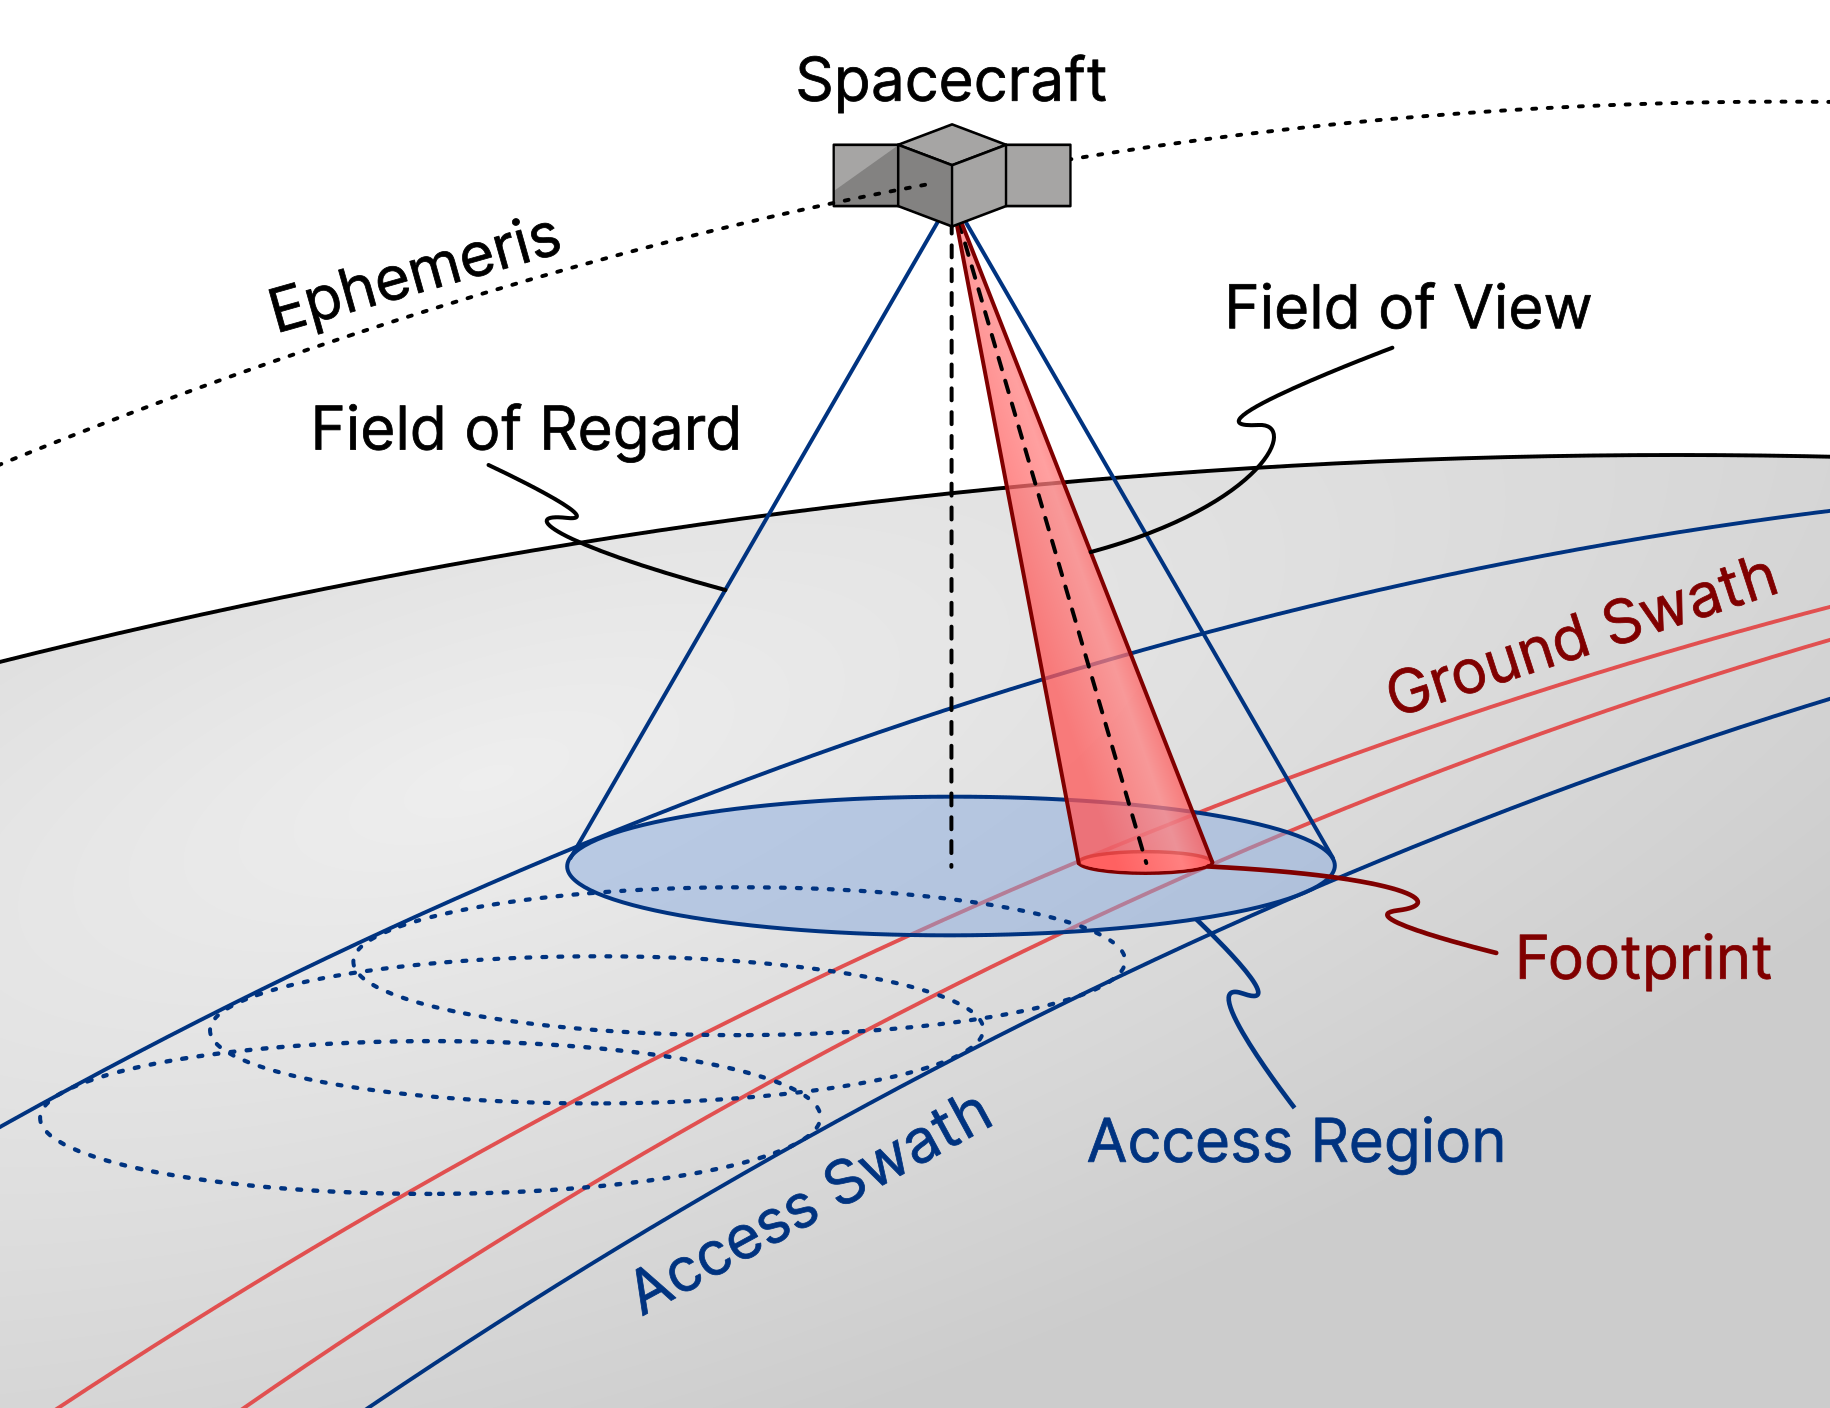
\includegraphics[width=\textwidth]{terminology.png} 
	\caption{General Illustration of Terminology}
	\label{fig:terminology} 
    \end{minipage}
    \hfill
    \begin{minipage}[c]{0.45\textwidth}
	\centering
	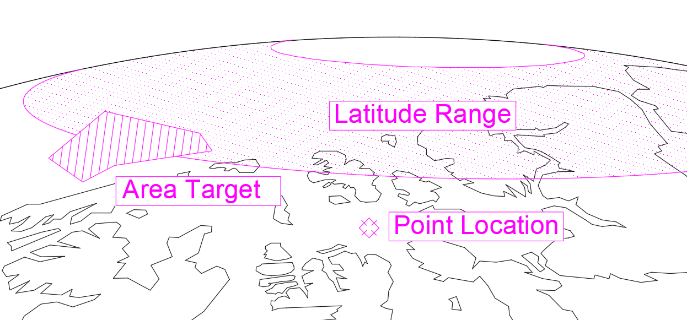
\includegraphics[width=\textwidth]{AOIs.png} 
	\caption{Different Types of Areas of Interest}
	\label{fig:AOIs} 
    \end{minipage} 
\end{figure}

%\begin{description} 
%
%    \item[Ephemeris] is a time series of orbital state vectors in a given
%	coordinate system. These state vectors have a position component,
%	$\sev{r}$, a velocity component, $\sev{v}$, and an epoch for each
%	vector, $e$. See section \ref{sgp4_section} for a more detailed
%	discussion on ephemerides.
%
%    \item[Area of Interest] An \gls{aoi} is a region on the Earth that is of
%	some particular importance to an operator. It is the region in which
%	one or more spacecraft should observe through some means. \glspl{aoi}
%	can be specified as a point location, an area target, or a latitude
%	range. Some examples of \glspl{aoi} are illustrated in \ref{fig:AOIs}.
%
%    \item[Field of View] The \gls{fov} is the extent to which a sensor or
%	instrument may observe the outside world at a given time. The size and
%	shape of an \gls{fov} varies based on the design of the sensor or
%	instrument. \glspl{fov} can theoretically describe any volume of space
%	but, for the purposes of this thesis, it may be assumed that they are
%	conical. Specifically, the \gls{fov} is defined by a single half-angle,
%	$\theta$. Suppose an instrument is pointing along some vector,
%	$\sev{u}$. Let us define another vector, $\sev{v}$ such that the angle
%	between it and $\sev{u}$ is $\theta$. The \gls{fov} is the volume
%	described by rotating $\sev{u}$ around $\sev{v}$.
%
%
%    \item[Field of Regard] The \gls{for} is similar to the \gls{fov} but
%	instead of being the area a sensor can observe in a single time
%	instant, the \gls{for} is the volume of space a sensor can possibly
%	observe by changing its orientation. Typically, it is constrained by
%	some physical or operational constraint. It is not possible to observe
%	the entire \gls{for}; Rather, only a subset of the \gls{for} can be
%	observed. This subset is the instrument's \gls{fov}.  For example, let
%	us consider an optical sensor fixed to a spacecraft orbiting the earth.
%	The position of the sensor at particular time instant is given by the
%	spacecraft's orbit and cannot be changed unless a propulsive manoeuvre
%	is performed.  Of course, the position of sensor can be changed
%	slightly by changing the attitude of the spacecraft, since the
%	instrument is most likely not located at the spacecraft's centre of
%	mass. But, this can be ignored since the distance the instrument can
%	translate is negligible compared to its orbit.  Conversely, The
%	orientation of the instrument can be changed, and this has a meaningful
%	effect on the \gls{for}. If no constraints are put on the attitude of
%	the spacecraft, the \gls{for} is everywhere, since the instrument can
%	be pointed in any direction. This is not always true though so let us
%	say the spacecraft can only point an angle, $\alpha$, off nadir.  The
%	\gls{for} would then be the cone described by the half-angle $\alpha +
%	\theta$, where $\theta$ is again the half-angle of the conical sensor.
%	Figure \ref{fig:fovfor} for an illustration of this example.  The
%	larger blue cone is the \gls{for}. The red cone is the sensor's actual
%	\gls{fov}. Its boresight is offset from the blue cone's.
%
%    \item[Footprint] The footprint is the area on Earth that can be observed by
%	an instrument's \gls{fov} or \gls{for} at a given time. It can be found
%	by intersecting the \gls{fov} or \gls{for} with the surface of the
%	Earth.  These intersection points form a boundary and the enclosed area
%	within this boundary is the footprint. For clarity, it should be
%	assumed that footprint refers to an \gls{for}'s footprint, unless
%	otherwise specified.
%
%    \item[Swath] If a sensor is moving over time, its footprint will move with
%	it. A swath is the union of all footprints over a time range.  It is
%	the region on Earth that can be possibly observed at some point by the
%	sensor.
%
%    \item[Horizon Swath] A horizon swath is a special case where the entire
%	Earth is within the sensor's \gls{for}. This may be true for certain
%	\gls{rf} payloads. In this case, the sensor can only `see' up until the
%	horizon. That is, the `horizon' footprint is all of the points on Earth
%	whose tangent line intersects with the sensor. Again, as the horizon
%	footprint moves, this forms the horizon swath.
%
%\end{description}



\section{Operations Scenario}

\gls{pops} is being developed to plan operations for missions at \gls{sfl}. To
maintain the privacy of their customers' operations strategies, an imaginary
scenario shall be introduced that is realistic but hypothetical. Given that
\gls{pops} is meant to be a general mission planning software, a hypothetical
mission scenario is still a valid example. Throughout this thesis, references
and examples will be made with this mission scenario in mind.

A common technique of remote sensing is Tip-and-Cue \cite{ali_tip_2021}.  In
this observation mode, multiple sensor systems are used to track both
stationary and moving targets over a wide area with high accuracy. First, a
sensor with a wide \gls{fov} is used to detect potential targets and these
targets are passed to another more accurate sensing system as ‘tips.’ The more
accurate system is then ‘cued’ to sense these potential targets. This is
especially useful for situations where the more accurate sensing system has a
limited \gls{fov}.

\begin{figure}[h]
    \centering
    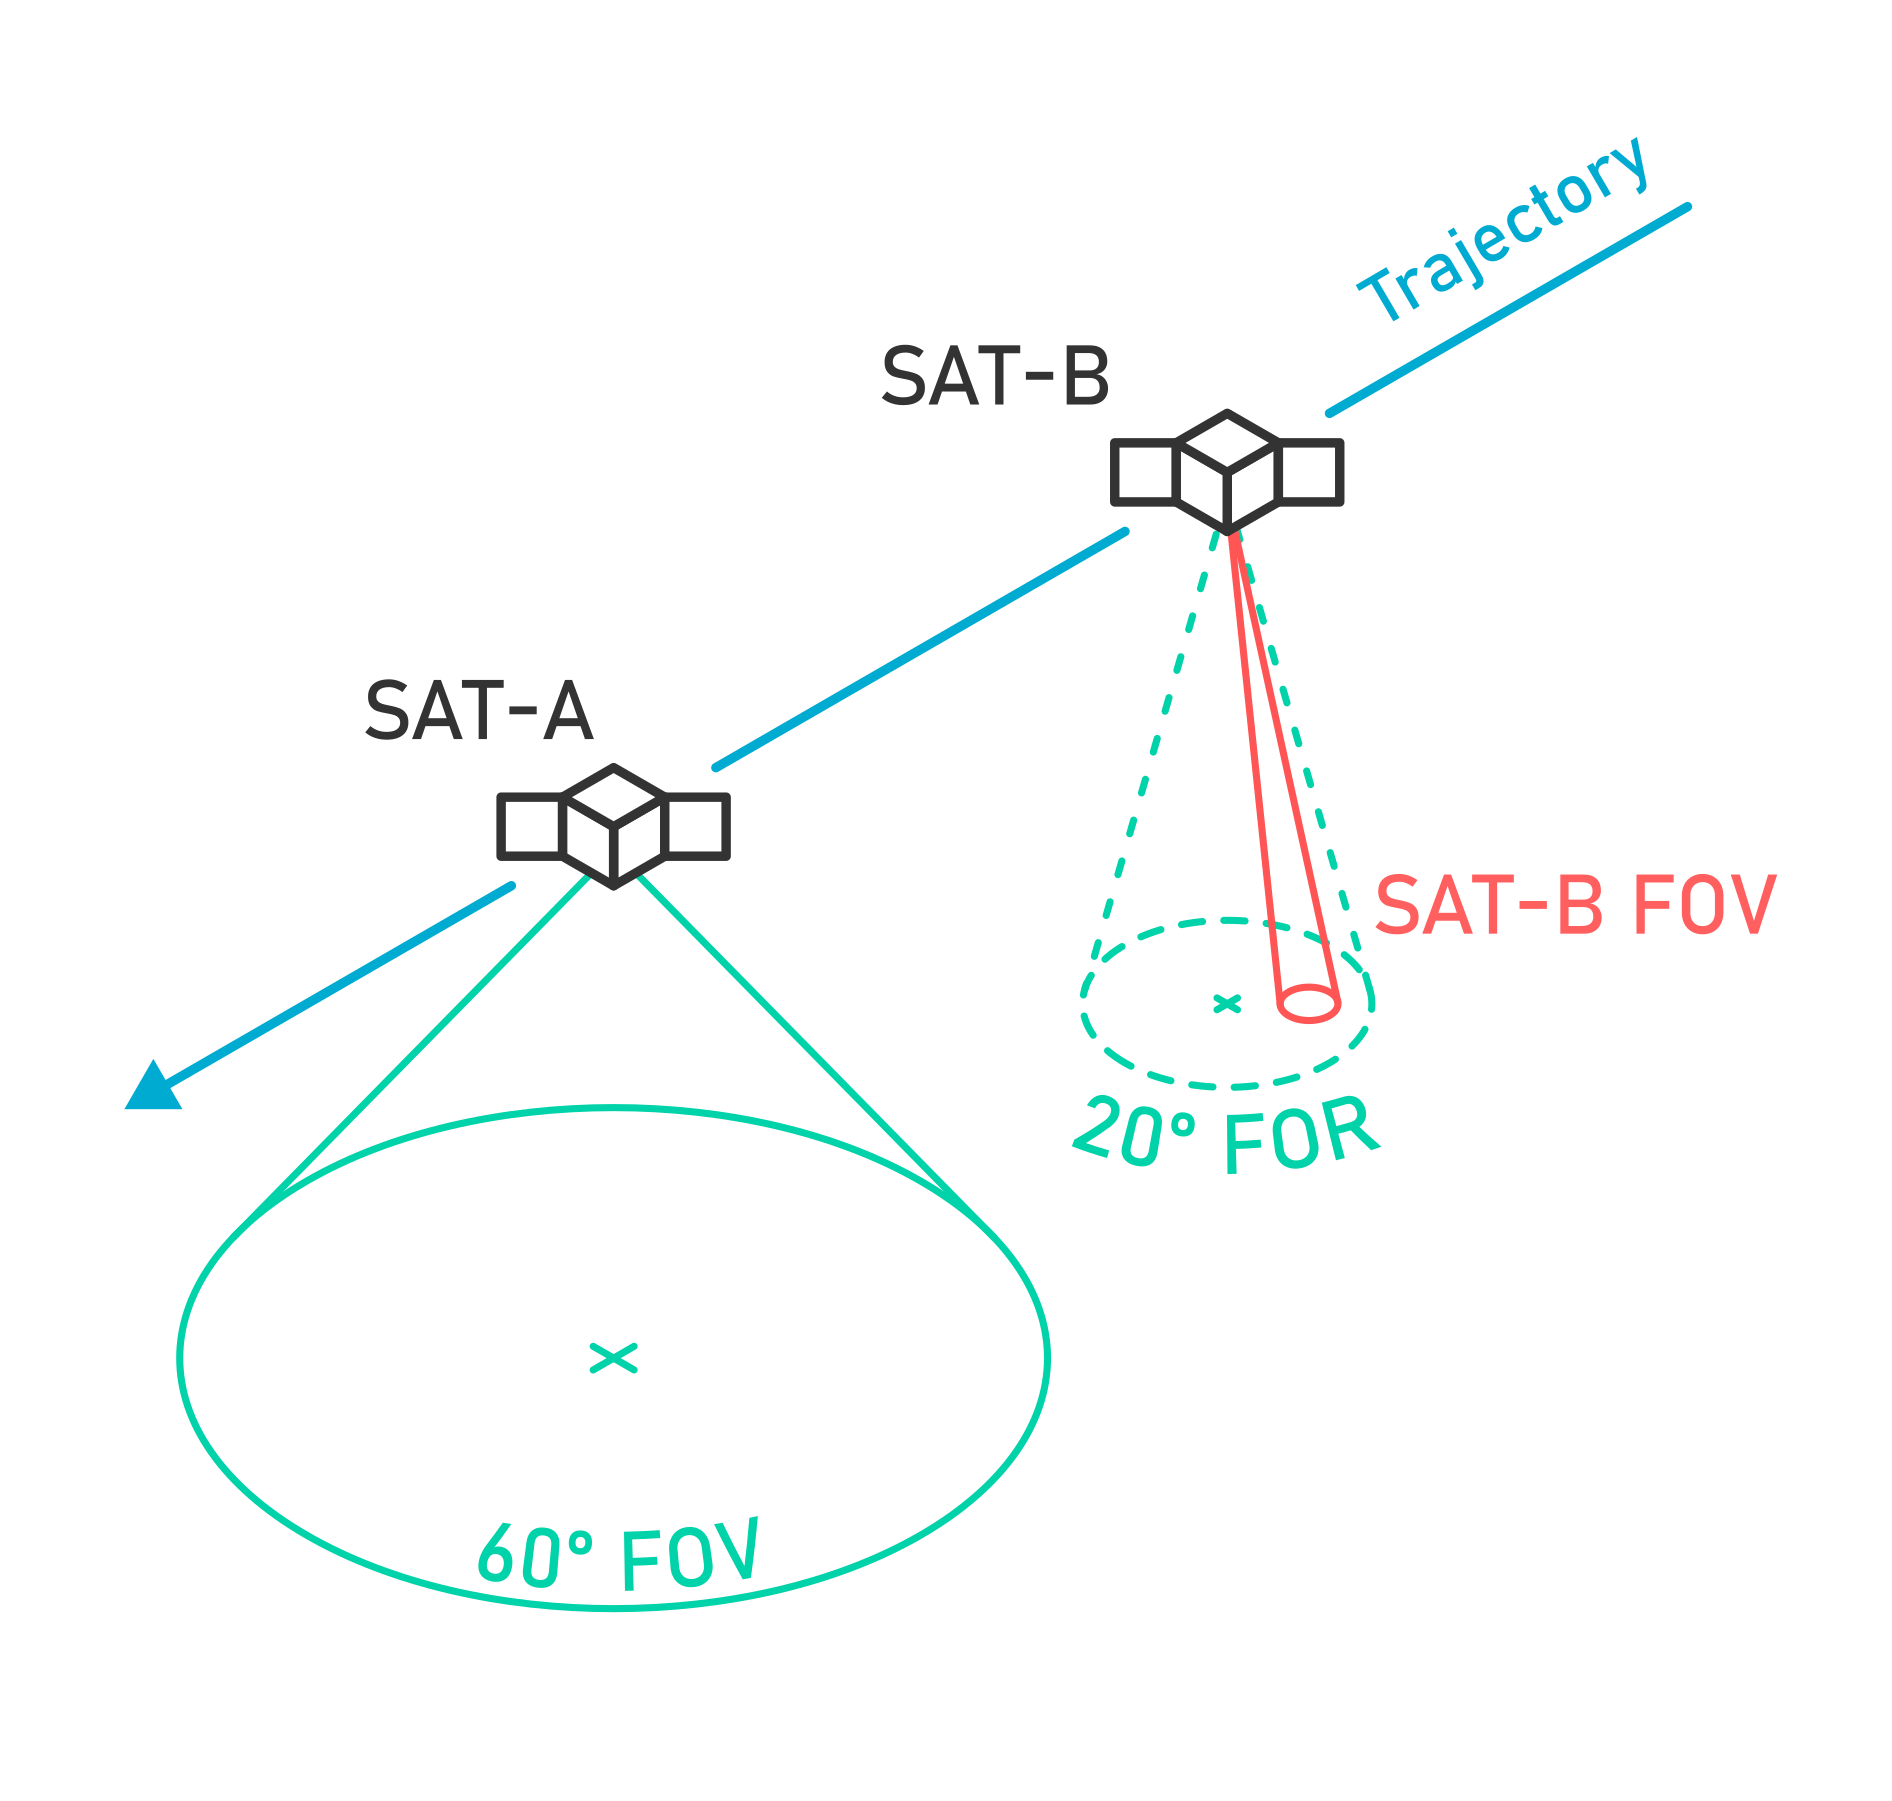
\includegraphics[width=0.6\textwidth]{EG-SAT.png} 
    \caption{EG-SAT Example Mission Scenario}
    \label{fig:eg-sat-1} 
\end{figure}

Let us say, as part of the “EG-SAT” mission, which is an imaginary mission, we
have a two-satellite constellation in formation where Sat-A leads Sat-B. Sat-A
has a course conical imager with a wide $60^\circ$ off-nadir \gls{fov} but low
ground resolution.  Sat-B has a fine conical imager with high ground resolution
but narrow \gls{fov}.  For the best coverage, Sat-A is always pointed at the
nadir.  Sat-B has some freedom and can be pointed $20^\circ$ off-nadir by
changing the spacecraft’s attitude.  It should be noted that since Sat-A’s
sensor is never pointed away from the nadir during payload operations, its
\gls{fov} is equivalent to its \gls{for}. Figure~\ref{fig:eg-sat-1} illustrates
the configuration of the EG-SAT mission.  The solid green lines under Sat-A
describe the $60^\circ$ \gls{fov} and footprint on the Earth. It is solid
because the \gls{fov} is equivalent to the \gls{for}. The dashed green lines
under Sat-B indicate the $20^\circ$ \gls{for} and access region. The red lines
indicate Sat-B's \gls{fov}. Notice how the \gls{fov} can be pointed in any
direction within the \gls{for}. This mission has two operations modes: 

\begin{figure} 
    \centering
    \begin{minipage}[c]{0.49\textwidth}
	\centering
	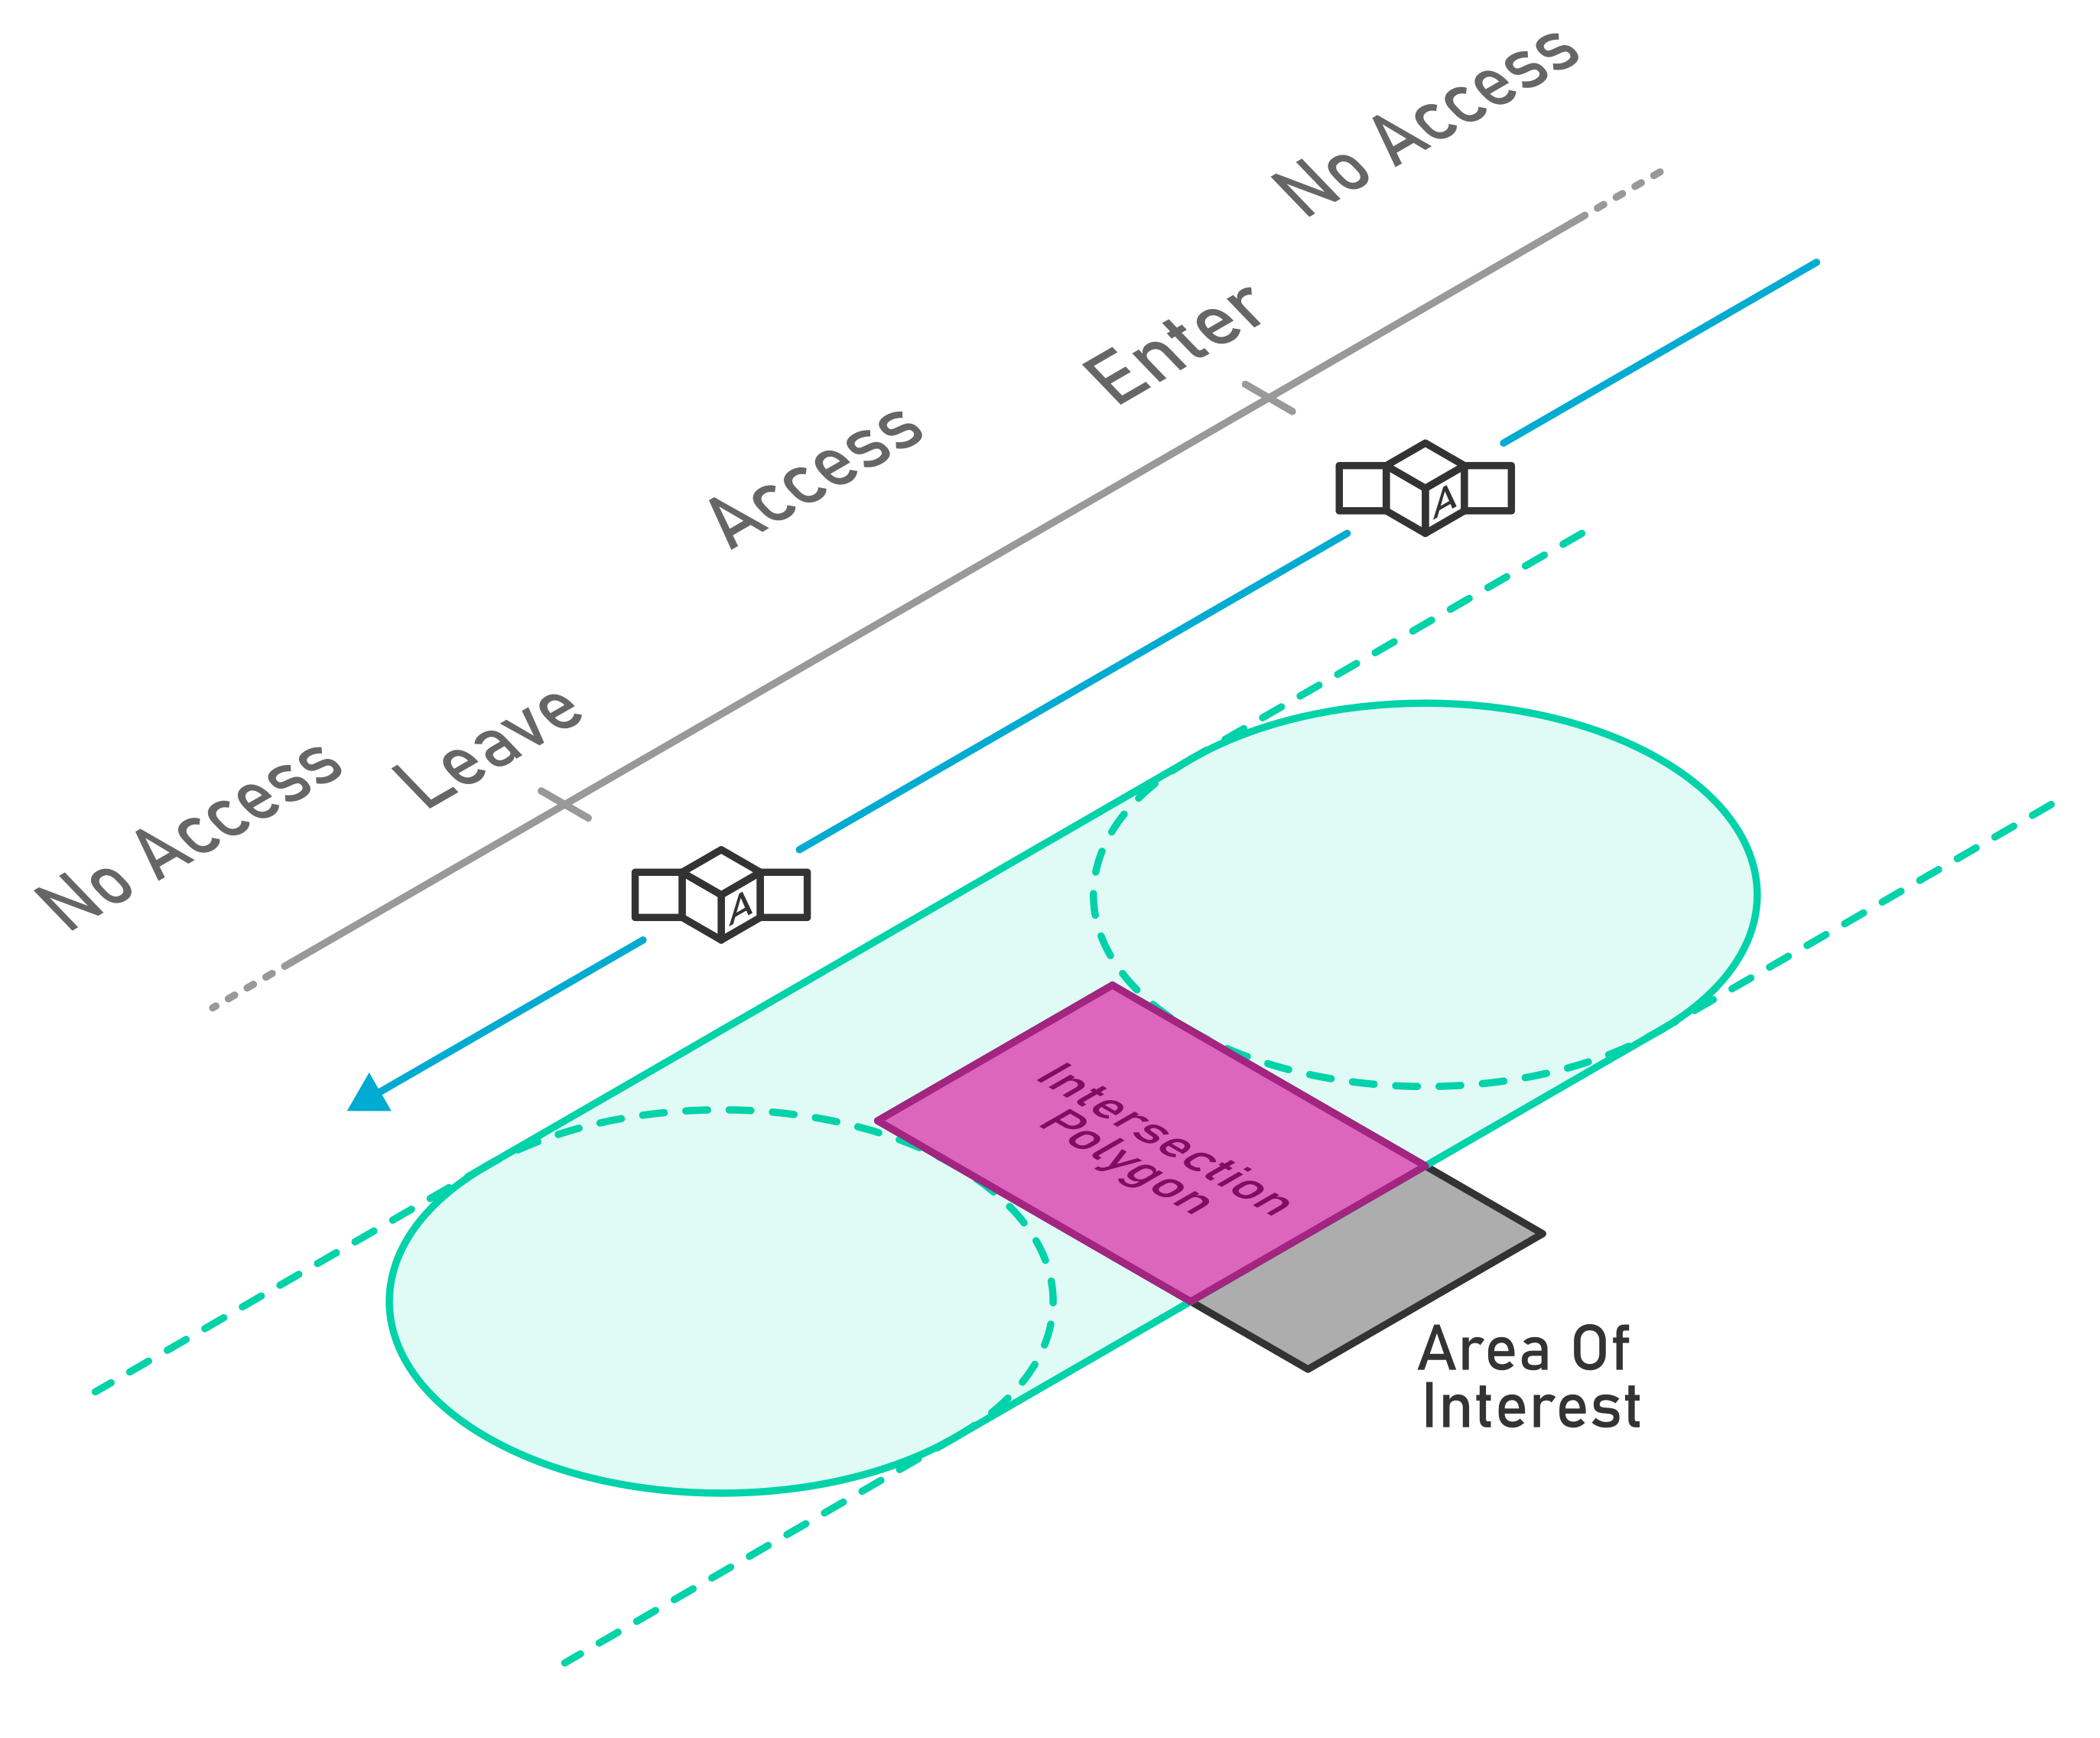
\includegraphics[width=\textwidth]{EG-SAT - obs 1.png} 
	\caption{Course Imaging}
	\label{fig:eg-sat-2} 
    \end{minipage}
    \hfill
    \begin{minipage}[c]{0.49\textwidth}
	\centering
	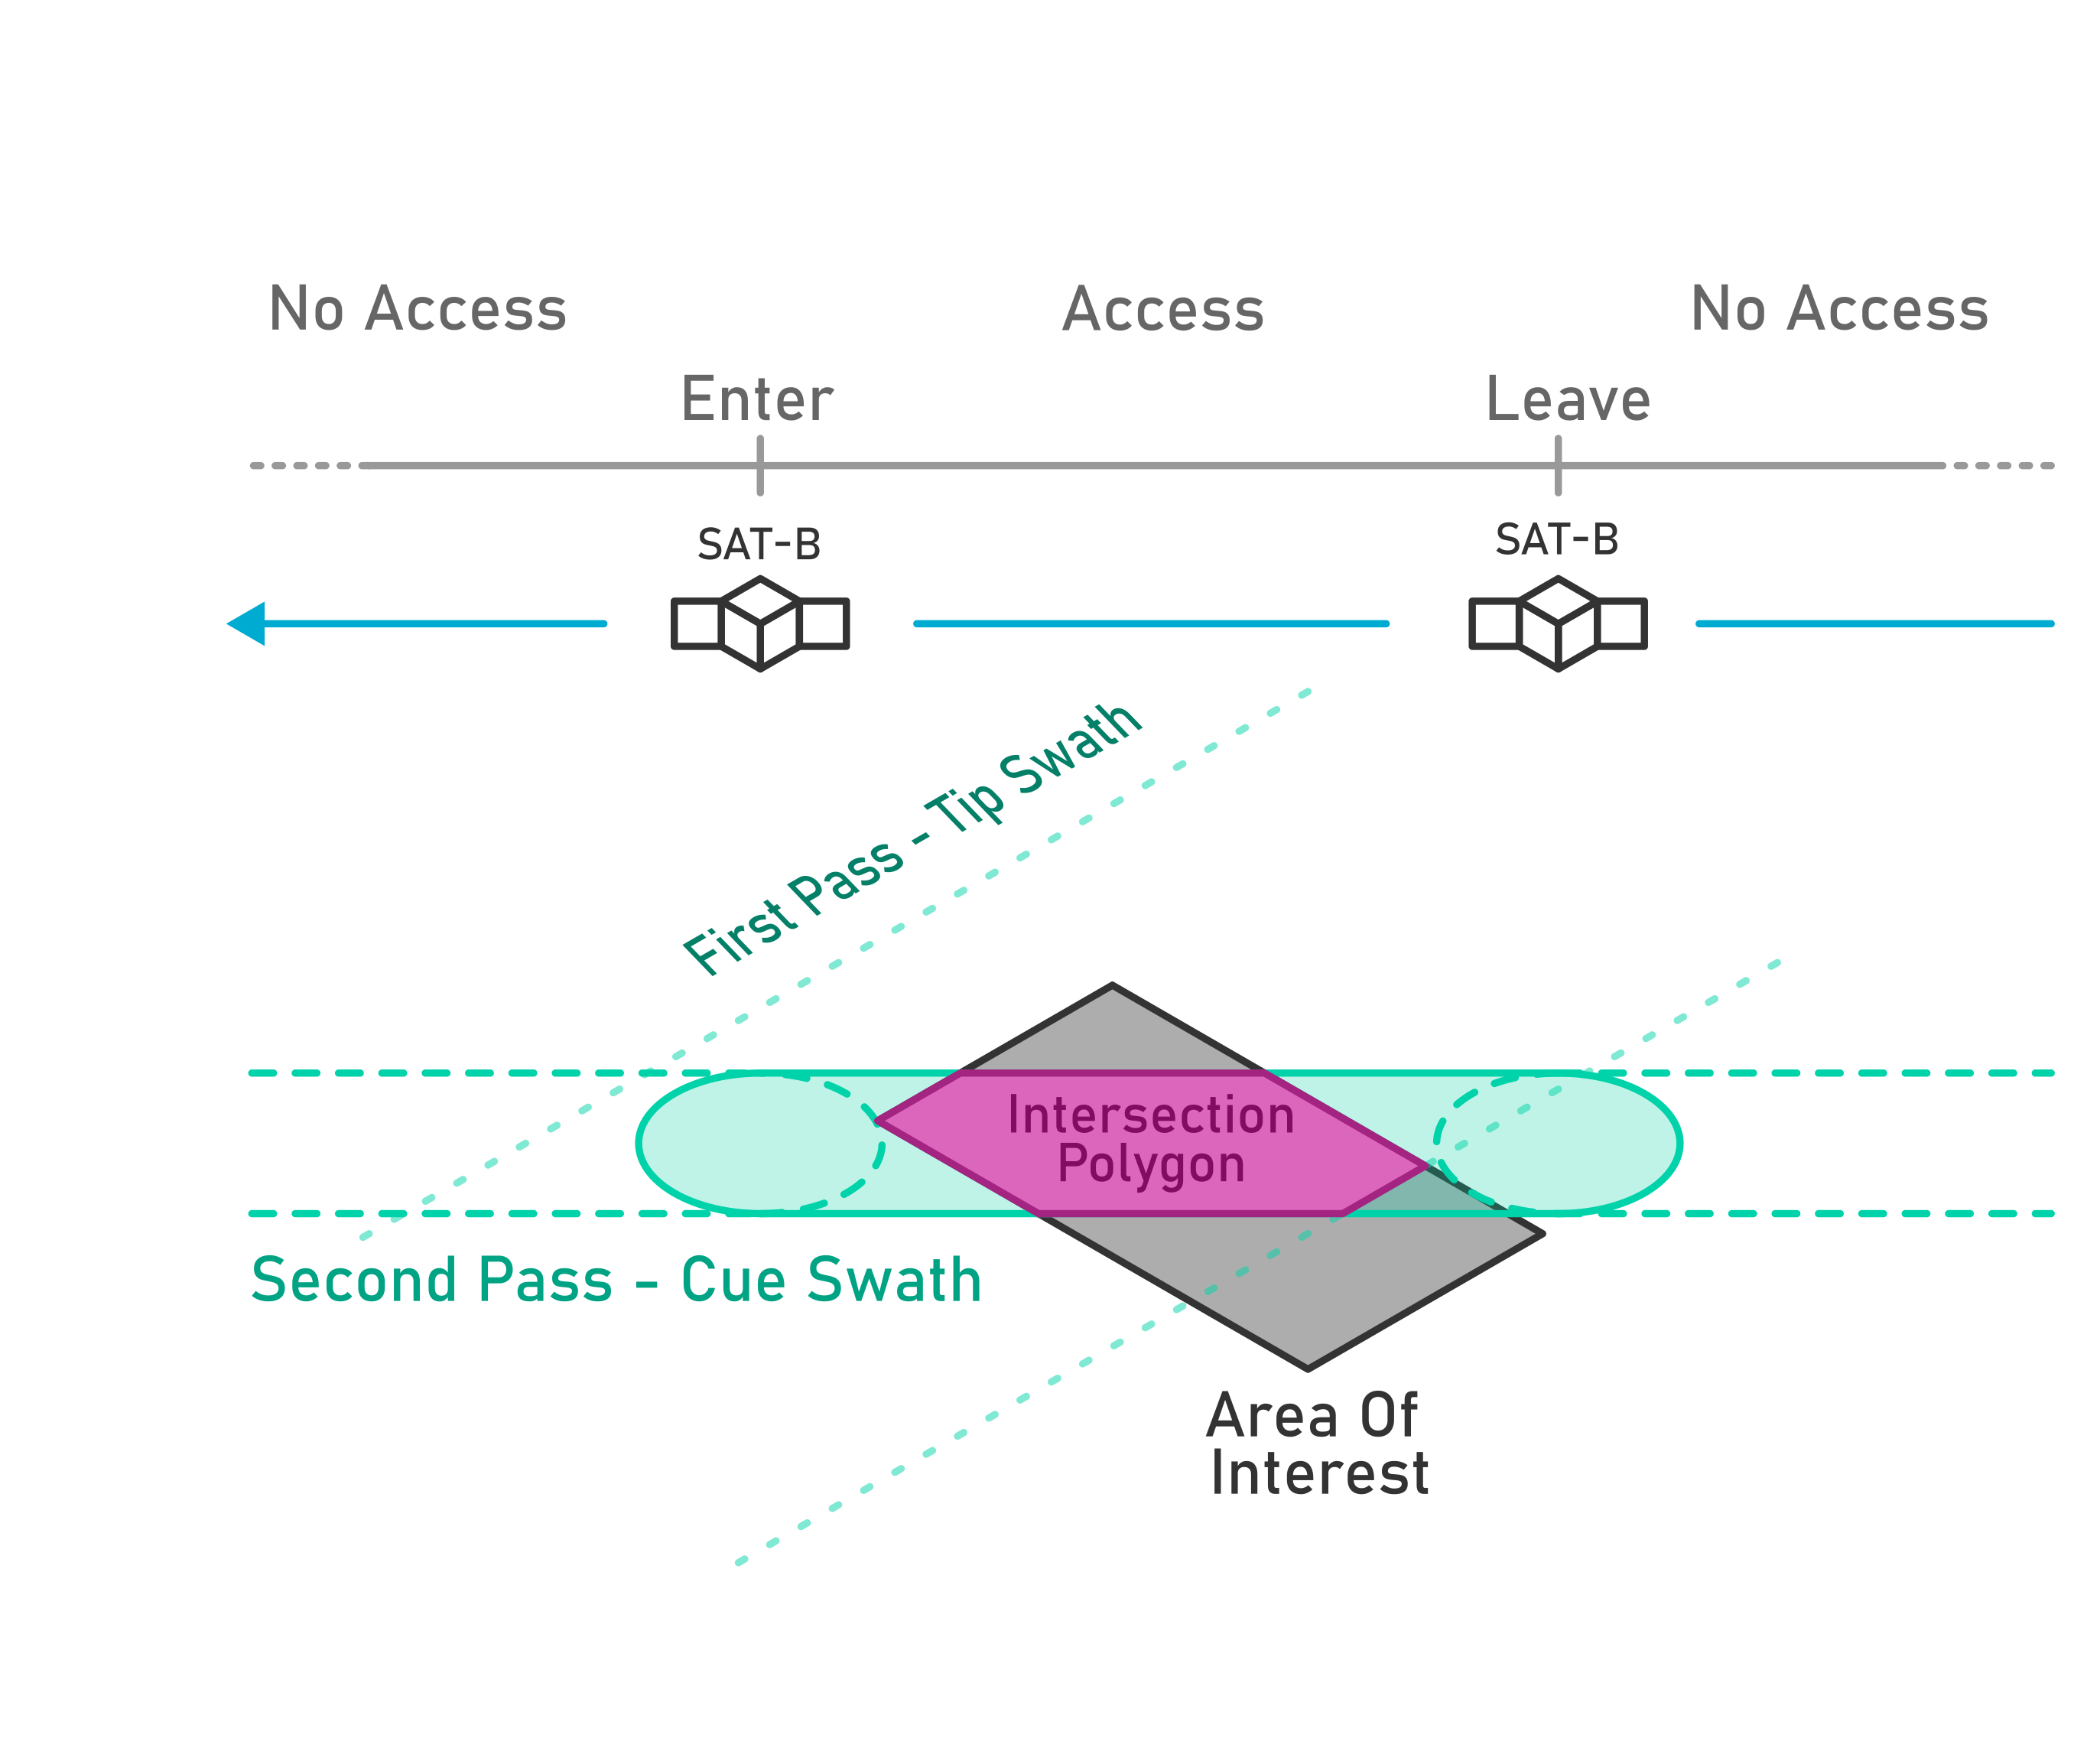
\includegraphics[width=\textwidth]{EG-SAT - obs 2.png} 
	\caption{Next-Pass Tip-and-Cue Imaging}
	\label{fig:eg-sat-3} 
    \end{minipage} 
\end{figure}


\begin{description} 

    \item[Course Imaging] In this mode, Sat-A must take images from all or part
	of an Area of Interest. This sensor data must then be recorded and
	downlinked at a ground station some time in the future.

    \item[Tip-and-Cue Imaging] Sat-A performs Coarse Imaging during the first
	pass over an Area of Interest. This data is then downlinked to a ground
	station which processes it and commands Sat-B to take fine images over
	the Area of Interest on the next pass.

\end{description}

The Course imaging mode is illustrated in Figure~\ref{fig:eg-sat-2}. When the
\gls{fov} of Sat-A first intersects the \gls{aoi}, Sat-A begins taking in
sensor data. This is represented by the solid green region.  When the \gls{fov}
no longer intersects the \gls{aoi}, Sat-A stops recording imagery data.
Typically for Area Target or Latitude Range \glspl{aoi} a satellite will not be
able to observe the entire area. As such, the region where the ground swath (or
access swath) intersects with the \gls{aoi} is called the Intersection Polygon
which is represented in magenta. 

The first pass of the Tip-and-Cue Imaging mode is equivalent to course imaging
and can still be seen in Figure~\ref{fig:eg-sat-2}. The next pass component
Tip-and-Cue Imaging mode is illustrated in Figure~\ref{fig:eg-sat-3}. It is
assumed that between the first and second pass, a ground contact has occurred and
Sat-B has been given fine imaging targets. Since, the location of potential
targets cannot be known a priori, we must rely on Sat-B's \gls{for}.  This
access region of Sat-B is represented by the green region in the Figure. For
this mode, the intersection polygon is not with the entire \gls{aoi}, rather it
is the Intersection Polygon from the previous pass. This is the area that
intersects both the \gls{aoi}, first pass ground swath, and next pass access
swath.  


\section{Opportunity Filtering} \label{sec:opp-filtering}

Opportunity Filtering is the process of taking an infinite set of potential
observations and filtering out opportunities based on a set of constraints.
Opportunities are instances or periods of time when a particular observation
mode can be performed on an \gls{aoi}. \gls{pops} is intended to be a
generalizable and easily expandable tool but the process of filtering for
observation opportunities is inherently specific to a mission’s operation’s
strategy.  For this reason, opportunity filtering functionality must be
developed individually for each operations mode.  Filtering may be done by
stringing together primitive utilities and saving the result. 

The inputs to the opportunity filtering process are: satellite ephemerides and
an \gls{aoi}. An opportunity filter may need to consider multiple satellites,
hence multiple ephemerides. These ephemerides form the basic component from
which all other search data is generated. It is from this search data that
\gls{pops} `filters' for opportunities. An \gls{aoi} must also be provided.
Without it, no opportunities can be found as an opportunity cannot exist
without an area to observe.

Let us now introduce our primitive utilities. By primitive utilities, it is not
implied that they are in any way simple or trivial to implement but, rather,
they form the most basic operations and cannot be simplified to another, more
basic, form.  These primitive utilities are implemented by the \gls{atu}
service which is discussed in Section~\ref{sec:atu} but for now they will be
discussed at a high level. For the EG-SAT mission, only three utilities will be
needed.

The first primitive utility is the \textbf{Swath Utility}. From a satellite
Ephemeris and the swath half-angle, the Swath Utility calculates the
corresponding swath over that time range. A half-angle is not the only way a
swath can be defined, but for this example scenario, it is assumed that swaths
are defined by conical \glspl{fov} or \glspl{for}. The swath that is generated
by this utility not only contains the bounded region of the swath but also the
footprint or access region at each time instant. Note, it has not been
specified whether the generated swath is an access swath or ground swath.  The
process for calculating either is equivalent, so a distinction is not made.  It
is up to the developer using the service to understand whether the outputted
swath is one or the other.

The second primitive utility is the \textbf{Polygon Intersection Utility}.
From a swath and a ground polygon, this utility calculates both the access
times and the intersection polygon between the swath and the input polygon. The
access times are timestamps which specify when a satellite `enters' or `leaves'
an access. The input polygon can be any polygon weather it is an \gls{aoi} or
it is derived through some other process.

The third primitive utility is the \textbf{Ground Access Utility}. From a swath
and a point target, this utility calculates the access times of the satellite
to the target. 

From these primitives, opportunity filtering will only output access times,
intersection polygons, or swaths. The concept of an `opportunity' is, to some
extent, completely arbitrary and not concretely defined. For \gls{pops}, an
opportunity may be represented through two components, \textit{where} and
\textit{when}. That is, what is the area that may be observed and when can one
or more spacecraft observe it. 

With a basic understanding of opportunity filtering, let us now walk through
defining filters for the two EG-SAT modes. For each filter it is helpful to
define: the inputs, required constraints, and what constitutes an opportunity.

\subsection{Course Imaging Filter}

\begin{description} 

    \item[Inputs:]  Sat-A Ephemeris and an \gls{aoi}

    \item[Constraints:] $60^\circ$ Ground Swath and an \gls{aoi}

    \item[Opportunity:] 1 Access Time (enter + leave) and 1 Intersection Polygon

\end{description} 

\begin{figure}[h]
    \centering
    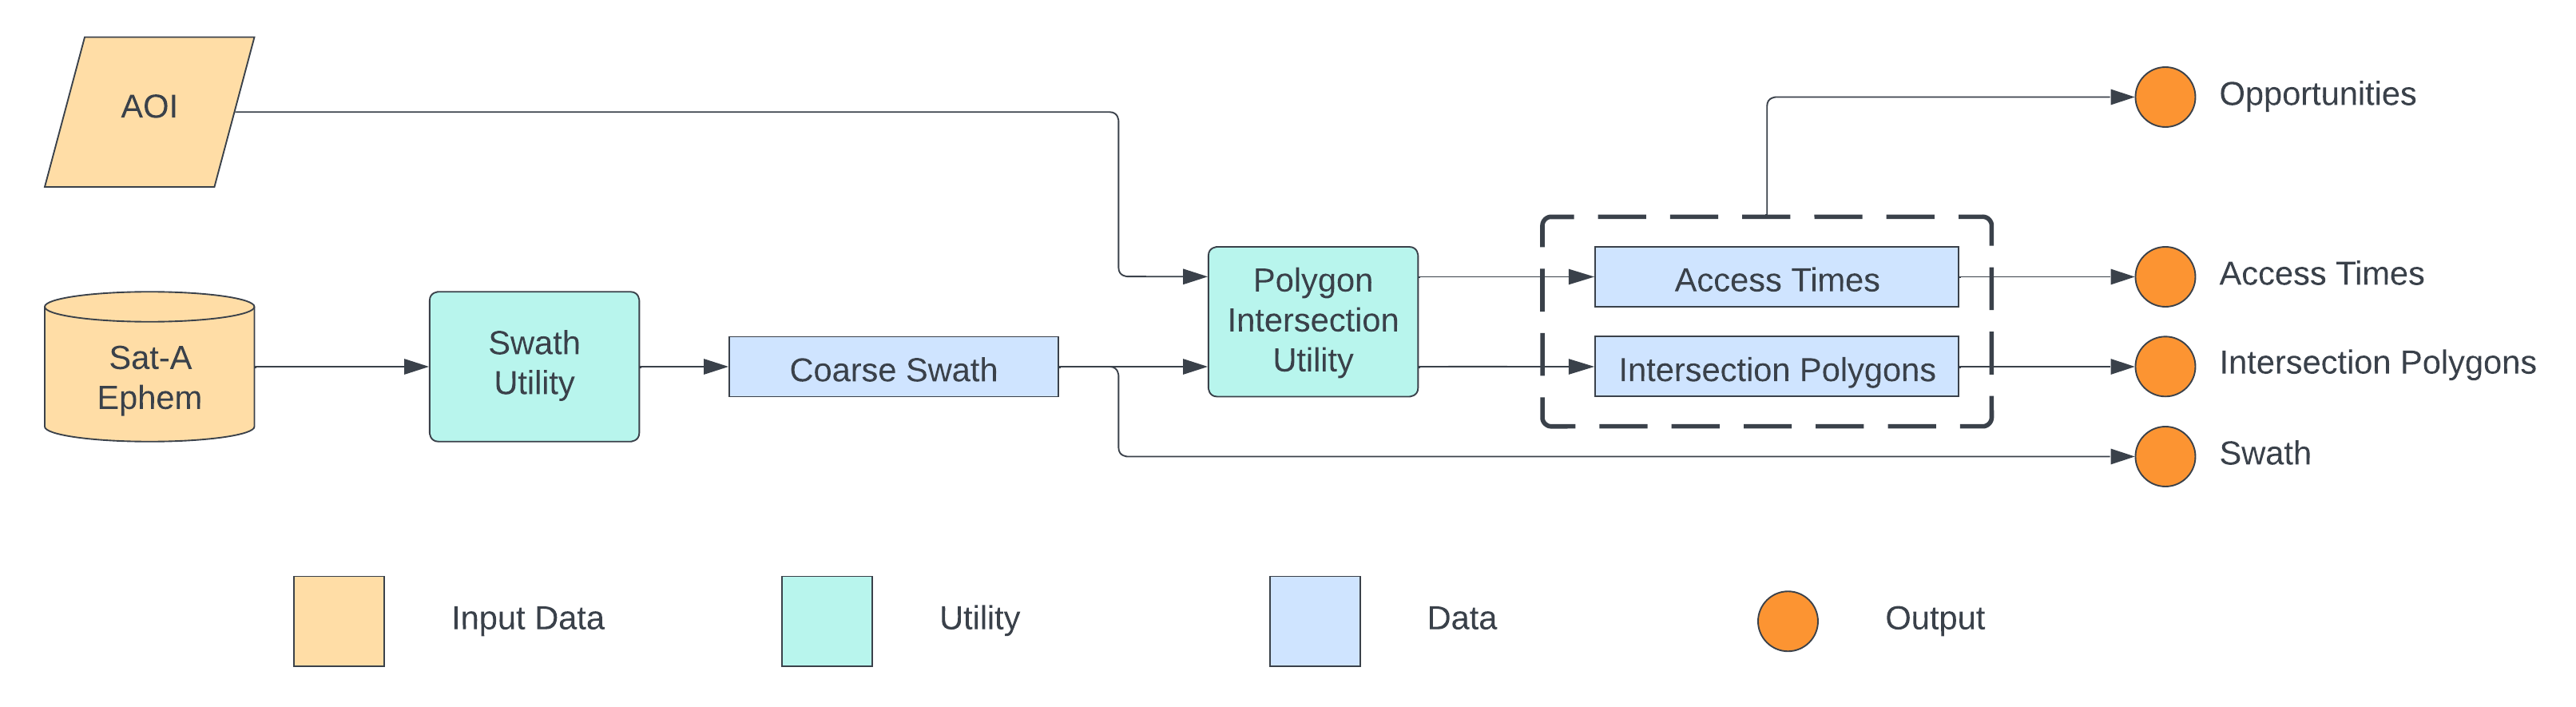
\includegraphics[width=\textwidth]{Coarse Imaging.png} 
    \caption{Coarse Imaging Filter}
    \label{fig:filter-1} 
\end{figure}

It is useful to display the filtering process graphically at a high level.
This can be seen in Figure~\ref{fig:filter-1}. First, from Sat-A's ephemeris,
its coarse imaging swath is generated using the Swath Utility. Then, the swath
is intersected with the \gls{aoi} through the Polygon Intersection Utility. The
output of which generates some access times and intersection polygons. When
these are generated, they are each linked together as opportunities. The
outputs of the filter are the opportunities, the access times, intersection
polygons, and swath data. All of this search data is recorded since it may be
referenced at a later point for displaying the results or for further
filtering.

\subsection{Tip-and-Cue Imaging Filter}

\begin{description} 

    \item[Inputs:]  Sat-A Ephemeris, Sat-B Ephemeris, and  an \gls{aoi}

    \item[Constraints:] $60^\circ$ Ground Swath (tip), $20^\circ$ Access Swath (cue), and an \gls{aoi}

    \item[Opportunity:] 1 Tip Access Time, 1 Cue Access Time and 1 Intersection Polygon

\end{description} 

\begin{figure}[h]
    \centering
    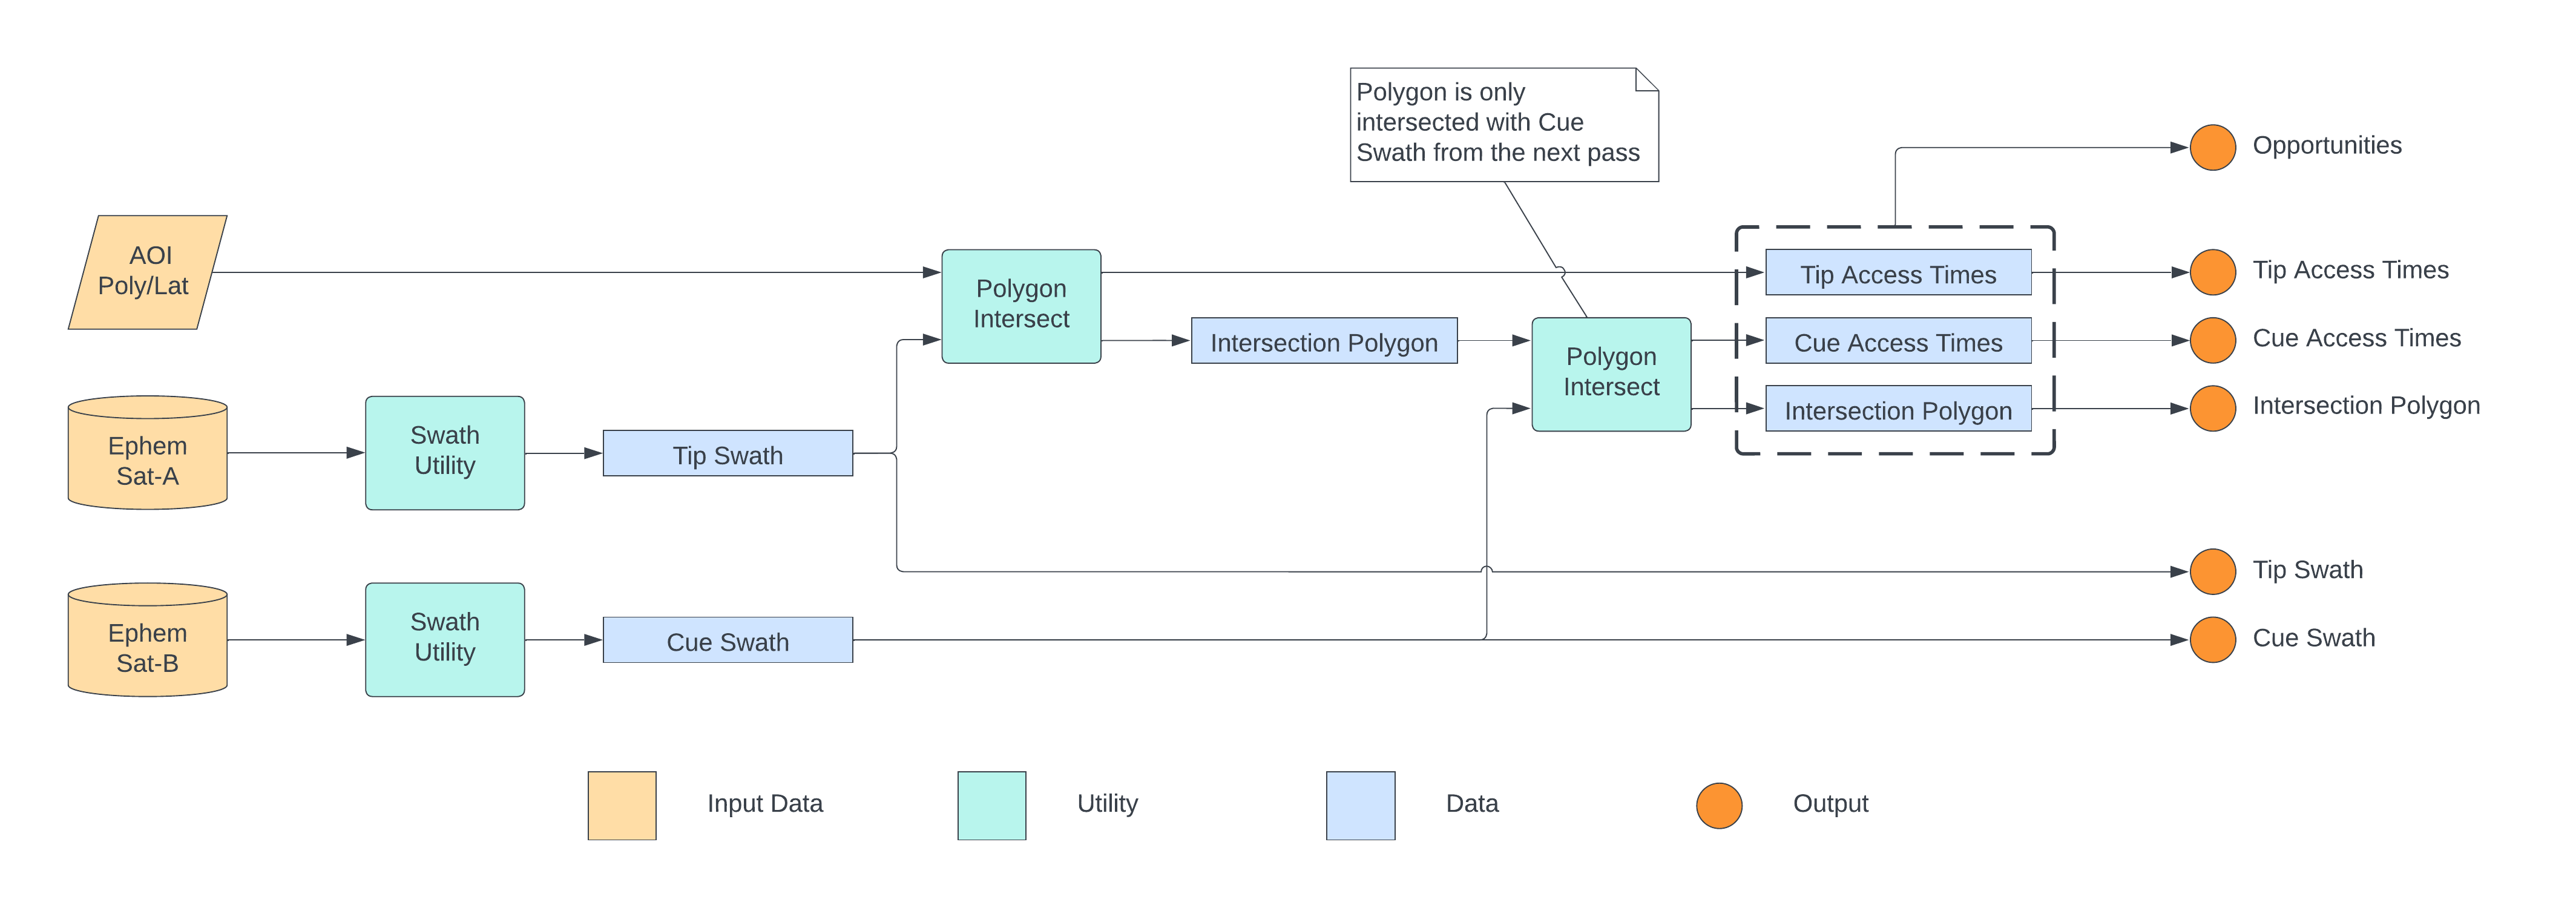
\includegraphics[width=\textwidth]{TNC Imaging.png} 
    \caption{Tip-and-Cue Imaging Filter}
    \label{fig:filter-2} 
\end{figure}


The Tip-and-Cue Imaging Mode can be seen in Figure~\ref{fig:filter-2}. The
first stage is the same as the Coarse Imaging filter. A tip swath, which is the
coarse imaging swath from Sat-A, is intersected with the \gls{aoi} to generate
access times and intersection polygons. In the second stage, Sat-B's ephemeris
is used to generate a cue swath, which is the fine imaging access swath. This
is then intersected with the intersection polygon from the previous stage. One
complexity that is hard to capture in the diagram is that the cue swath must be
subdivided into passes, such that it can be intersected on the next pass. From
the second Polygon Intersection Utility, Cue Access Times and final
intersection polygons are produced. These are linked together with the Tip
Access Times from the previous pass. All of this information is then outputted
along with the Tip and Cue Swaths.

This was a high-level overview of how Opportunity Filters are constructed. How
they are implemented and how the output data is used is discussed in the next
chapter.


\section{Orbit Propagation}

For \gls{pops}, it is essential that there is some way of propagating a
satellite's orbit. That is, there must be a way of estimating a satellites
position at a given time.  Very accurate methods of propagation do exist, but
these are involved and may be time consuming to implement. The desire for
\gls{pops} currently is to have \textit{some} method of propagation that is
sufficiently accurate.

\subsection{NORAD Two-Line Element Sets}

The United States Space Force tracks all detectable Earth \glspl{rso} and makes
this information public in the form of lists of \gls{norad} \gls{tle} sets.
\glspl{rso} are any natural or artificial object in Earth's orbit or any other
body.  This information is one of the only public sources of data regarding
Earth orbiting \glspl{rso}. Among these \glspl{rso} are \gls{sfl} spacecraft. A
\gls{tle} is a standard data format that contains a list of specialized orbital
elements at a specific time, referred to as the \gls{tle} epoch. \glspl{tle}
are inextricably linked to the `simplified perturbation models' family of
algorithms, specifically \gls{sgp4}.  Though less accurate than numerical
computation methods, these allow for quick and relatively accurate computation
of satellite trajectories.  This section is not intended to be an in-depth
reference of propagating satellite trajectories with \glspl{tle} but rather it
is a summary of the concepts as well as some of the literature.

Unfortunately, there have not been many publications made by the U.S. military
regarding the exact process to generate \glspl{tle}. This is essential because
the assumptions made in the creation of a \gls{tle} must be accounted for to
produce accurate propagation results. There are, though, a few publications of
note on this subject. Originally the source code for the `simplified
perturbation models' family of algorithms was defined explicitly in
\cite{hoots_spacetrack_1980}.  After some years, many purpose-built versions of
\gls{sgp4} were developed, each with their own assumptions and implementation
details. These were consolidated together in \cite{vallado_revisiting_2006},
which provided a number of tested implementations of \gls{sgp4} in a variety of
programming languages. Still today, this is the best reference for \gls{sgp4}.
Later, \cite{vallado_sgp4_2008} was published as a reference for generating
\glspl{tle} from ephemeris data. In addition, \cite{vallado_fundamentals_2001}
was published as an exhaustive reference on orbital dynamics which discusses at
length not only \glspl{tle} and \gls{sgp4} but also the underlying theory as
well as derivation examples.



\begin{figure}[h]
    \begin{verbatim}
    IDENTIFIER
    1 16609U 86017A   93352.53502934  .00007889  00000-0  10529-3 0  0342
    2 16609  51.6190 13.3340 0005770  102.5680 257.5950 15.59114070 44786
    \end{verbatim} 
    \caption{Example of a \gls{tle}}
    \label{fig:tle-ex} 
\end{figure}

An example of a \gls{tle} can be seen in Figure~\ref{fig:tle-ex} taken from
\cite{vallado_fundamentals_2001}.  As the name implies, there are two
69-character lines of data. Occasionally, a title is added for reference but
this is not required as part of the \gls{tle} definition. The data allocations
can be seen in Figure~\ref{fig:tle-legend}. The corresponding allocations for
each reference number can be seen in Table~\ref{tab:tle-line-1} and
Table~\ref{tab:tle-line-2} for lines 1 and 2 respectively.

\begin{figure}[h]
    \centering
    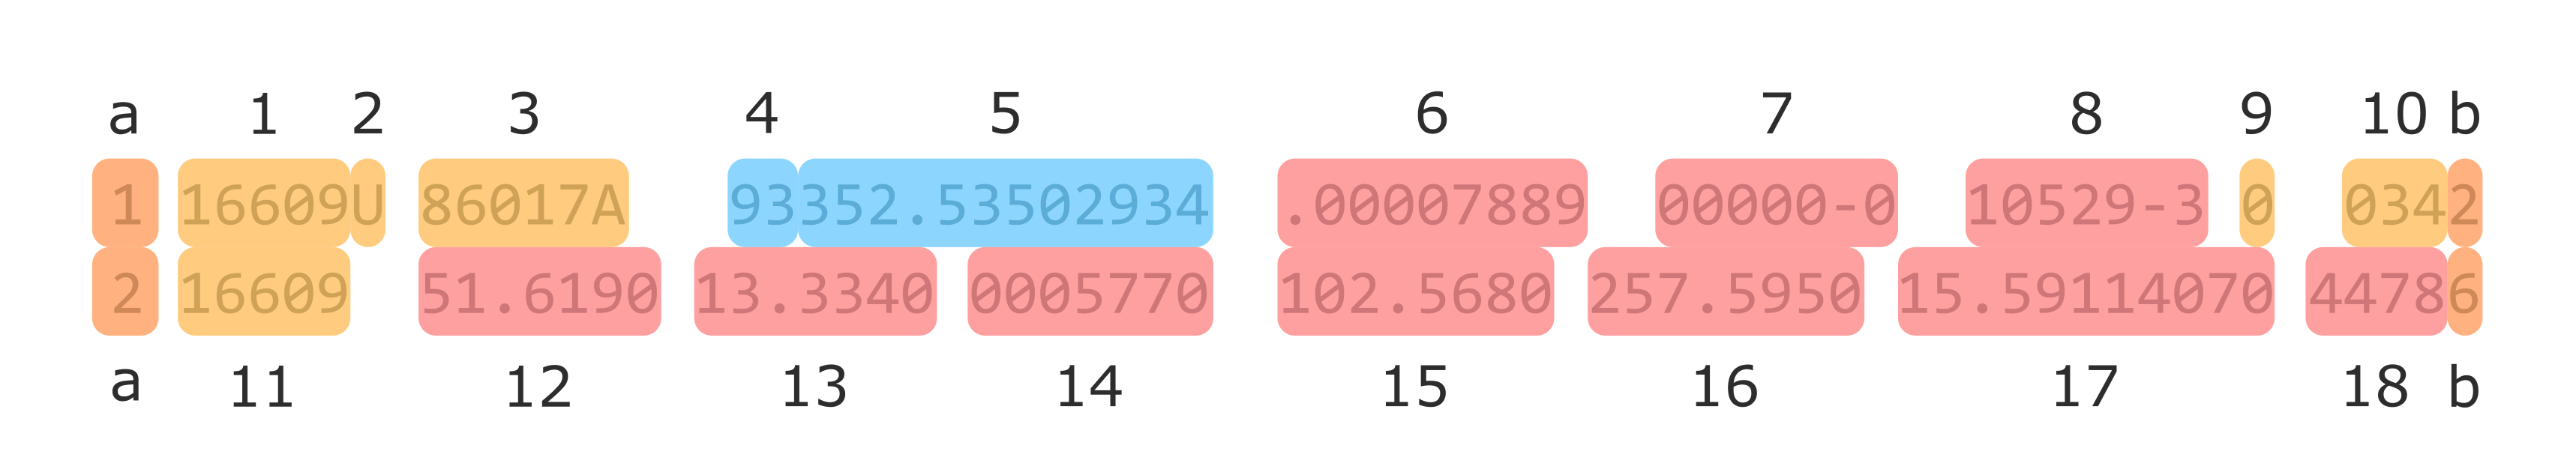
\includegraphics[width=\textwidth]{TLE.png} 
    \caption{TLE Data Format}
    \label{fig:tle-legend} 
\end{figure}

\begin{table}[!htb]\small
%\setlength{\tabcolsep}{6pt}

\begin{minipage}{.49\textwidth}
\centering

\caption{Data Format, Line 1}
\label{tab:tle-line-1}

\medskip

\begin{tabular}{|c|ll|}
\hline

\multicolumn{1}{|l|}{} & \multicolumn{1}{l|}{Description} & \multicolumn{1}{l|}{Units} \\ \hline
a  & Line Number   &   \\ \hline
1  & Satellite Number   &   \\
2  & Classification (U/C/S)   &   \\
3  & International Designator   &   \\
4  & \gls{tle} Epoch, Year   & years  \\ 
5  & \gls{tle} Epoch, Day   & days  \\
6  & Mean Motion, $1^{\mathrm{st}}$ Derivative & rev/day  \\
7  & Mean Motion, $2^{\mathrm{nd}}$ Derivative    & rev/day$^3$  \\
8  & B* (B Star)   & $R_{\mathrm{Earth}}^{-1}$  \\
9  &  Ephem Type (always 0)  &   \\
10  &  Element Number  &   \\ \hline
b  & Checksum   &  \\
\hline

\end{tabular}
\end{minipage}\hfill
\begin{minipage}{.49\textwidth}
\centering

\caption{Data Format, Line 2}
\label{tab:tle-line-2}

\medskip

\begin{tabular}{|c|ll|}
\hline

\multicolumn{1}{|l|}{} & \multicolumn{1}{l|}{Description} & \multicolumn{1}{l|}{Units} \\ \hline
a  & Line Number   &   \\ \hline
11 & Satellite Number   &   \\
12 & Inclination   & $^\circ$  \\
13 & Right Ascension   & $^\circ$  \\
14 & Eccentricity &   \\
15 & Perigee & $^\circ$  \\
16 & Mean Anomaly & $^\circ$ \\
17 & Mean Motion & rev/day \\
18 & Orbit Number &  \\ \hline
b  & Checksum   &  \\
\hline

\end{tabular}
\end{minipage}


\end{table}

It is not essential to have a complete understanding of every term in a
\gls{tle}. Generally, they are meant to be consumed by an algorithm and are not
human readable. Despite this, it is good to have a general understanding of the
terms.  Elements 1-3 and 11 give information about the satellite the \gls{tle}
has been generated for. Elements 4 and 5 give the \gls{tle} epoch.  Elements
12-17 give the independent orbit elements that can be used to describe a
satellite's orbit. Elements 6-8 describe the effects of perturbations on that
orbit. Lastly, Elements a, b, 9, and 10 give meta-information about the
\gls{tle} itself. Even though the orbital elements of a satellite can be
extracted from a \gls{tle} and can then be used as inputs for another
propagator, this would be a mis-step and would produce erroneous results. 

\begin{quote}
[\glspl{tle}] are `mean' values obtained by removing
periodic variations in a particular way. In order to obtain good predictions,
these periodic variations must be reconstructed (by the prediction model) in
exactly the same way they were removed by \gls{norad}. Hence, inputting
[\glspl{tle}] into a different model (even though the model may be more accurate or even
a numerical integrator) will result in degraded predictions. \cite{hoots_spacetrack_1980}
\end{quote}


\subsection{Propagator}

Within the simplified general perturbations family of algorithms there are 5
orbital propagation models: SGP, SGP4, SDP4, SGP8, and SDP8. These are
analytical methods of approximating orbital state vectors at corresponding
epochs. SGP (Simplified General Perturbations) was originally developed in 1966
for near-Earth satellites (orbital periods less than 225 minutes). It was then
replaced by SGP4 and SDP4.  SGP4 was originally developed in 1970 for near
Earth Satellites and SDP4 was an extension for `deep-space' satellites (orbital
periods greater than 225 minutes) in 1979.  The SGP8/SDP8 models were developed
in 1980 to address deficiencies in the previous versions but ultimately, they
did not become widely used.  Today SGP4/SDP4 are the dominant models.  Since
there is a clear distinction between when SGP4 and SDP4 should be used, they
are collectively referred to as just `SGP4'. Since the original report
\cite{hoots_spacetrack_1980}, changes have not been made to the theory but
rather the code implementations.  It should be noted that \glspl{tle} are
accurate to around a kilometer at epoch and degrade rapidly
\cite{vallado_revisiting_2006}. The actual error of an individual \gls{tle}
varies on a case by case basis. One source of error is that \glspl{tle} should
be generated based on maneuver free arcs of ephemeris. The valid time horizon
of a \gls{tle} is greatly truncated by any unaccounted for perturbations
imposed on the orbit. If some thrusting is done by a spacecraft to maintain a
formation, for example, \glspl{tle} generated before the maneuver will not
account for the orbit variation induced by this perturbation. After this
thrust, new \glspl{tle} will need to be generated.

%maneuvers cannot be taken into account when generating \glspl{tle}. If some
%thrusting is done by a spacecraft to maintain a formation, for example,
%\glspl{tle} generated before the maneuver will not be accurate after the
%thrust has occurred. After this thrust, new \glspl{tle} will need to be
%generated. 



\subsection{Coordinate Systems}

When using Earth-centric coordinate systems, there are generally two types:
\gls{eci} and \gls{ecef}. These are not reference frames themselves but only
refer to families of reference frames. They vary based on the exact definitions
for each axis.  \gls{eci} frames do not move with the Earth's rotation; they
remain, as the name implies, inertially fixed and their axes are defined with
respect to celestial bodies. \gls{ecef} frames do move with the Earth's
rotation. As such, they are useful for Earth-sensing satellite operations since
coordinates in an \gls{ecef} frame can be directly converted into
Latitude-Longitude-Altitude coordinates, whereas with an \gls{eci} frame this
process is more involved. The outputs of the \gls{sgp4} propagator are in the
\gls{teme} coordinate reference frame which is an \gls{eci} reference frame.
\gls{teme} is not particularly useful and must be transformed.  This process is
discussed later.



\section{Time Tag Commands}

At the \gls{sfl}, satellites are commanded through the use of the \gls{nsp}
\cite{kekez_nanosatellite_2010}.  \gls{nsp} commands are a custom standard
developed by \gls{sfl} to facilitate ground and intra-satellite communication.
They are designed to minimize the effects of low-bandwidth radio communication
links that are prone to error.  These commands handle all aspects of nominal
operation, from turning individual units on or off, to specifying attitude
modes or initiating data transfers.  Once a command is sent, it is executed
immediately upon being received. This raises the concern for how a spacecraft
can be commanded when it does not have a direct communication link with a
ground station. To address this, there exist \glspl{ttc}.  \glspl{ttc} are
\gls{nsp} commands that have been prepended with a timestamp and a group ID.
When the spacecraft’s system clock reaches the time specified in the timestamp,
that command is executed.  The group ID allows operators to group \glspl{ttc}
such that they may be considered as a collection rather than as separate
commands, allowing for reference or removal as a single unit.  \glspl{ttc} are
prepared in advance by an operator and uploaded in bulk to the spacecraft.
This allows operators to control the spacecraft when direct communication
cannot be established.




\glsresetall{} 
\chapter{Software Architecture}\label{chap:architecture}


\section{Payload Operations Planning Software Architecture}

The \gls{pops} is made up of several distinct components separated into
services.  Each service has its own Docker5 container. Containers are similar
to virtual machines in that they simulate an operating system but, unlike
virtual machines, they do not simulate the underlying hardware. This makes
containers much more lightweight, while also retaining the benefits of having a
standardized environment where dependencies are packaged with their source
code. Containers make deploying and maintaining \gls{pops} much easier since
installation does not require managing dependencies and tweaking environment
variables. In this way, a \gls{pops} user does not need to be as familiar with
the software as a developer to run it. Each service is its own Python web
server. In this way, they may be interacted with via a RESTful API. That being,
HTTP requests can be made to retrieve information or perform calculations. Each
service also provides its own automatically generated documentation that can be
accessed through a web browser. This documentation outlines possible API calls
as well as their input and output data formats.  This allows a user to quickly
see the capabilities of a service without accessing the source code. Currently,
\gls{pops} has 4 main services; they are the: Mission Model, Propagator,
Database, and Access Time Utilities,  Mission Model.

%% ======================================================================== %%
%%			    General Architecture
%% ======================================================================== %%

\section{General Service Architecture}

Every service contains the same basic components so it is worth discussing
services generally and then going into specifics in subsequent sections. These
components are: the dockerfile, a main Python script, a models file, service
specific scripts.

To review, a docker container is a virtual environment, which is a simulated
operating system. A container can be created from an image and an image canbe
built from a Dockerfile. As such, the Dockerfile is the fundamental text
document that is used to assemble an image. It specifies: the operating system
that should be used, what files should be included in the container, and what
commands should be run upon container creation. By specifying an operating
system, we can tailor a service to any environment that best suits the service's
needs. They can use windows, the latest version of Ubuntu, or a lightweight
tailored linux distrubution that only contains the tools a service needs. In
this way, one service can be running Ubuntu 20.04 for ease of development, and
another service can be running Windows 10. In this way, \gls{pops} is not
limited by the operating system it is developed in. Files may  be added to a
container simply by pointing to their location in the host's file system upon
image creation. Finally, when a container is first created from an image, a
conatiner will need to install all of the necessary dependencies. In general,
this will either be Ubuntu packages, a version of Python, and Python libraries.
In this way, dependencies can easily be tracked. The last command that is
executed is the command that starts a service's main script.

Theoretically, all of the code for a service could live in the main Python file
but, if this were the case, it would quickly balloon and become unwieldy to work
with so functionality is split into multiple scripts. The main script serves a
number of functions. Its purpose is to handle all of the web-server aspects of
the service. Functions such as: creating the web-server, setting server
parameters, setting up environment variables, and handling API calls. Setting up
the webserver is fairly straightforward since open source libraries are used to
handle all of the low-level functionality and implementation. What is most
important is specifying potential HTTP requests. These requests are how a
service may be interacted with by a user, their browser, or by other services.
The parts that must be specified are the: 

\begin{itemize}
    \item Request type (GET, POST, PUT, etc.), 
    \item Path to the request, 
    \item Response type (JSON, Plain Text, HTML, etc.), 
    \item Input variables if applicable, and the 
    \item Function that is called when a request is received.
\end{itemize}

For GET requests, the input variables are generally straightforward since the
only input variables that can be used must be explicitly stated in the request
itself. But, for POST requests or other requests that contain information in
the body of the request, the format of the input data must be defined or else
the web server will fail the request as being unprocessable. These input
definitions are stored in the models file. Python is a dynamically typed
language so variables do not need to be assigned a type upon creation. To
ensure input data conforms with what is expected by the api, the Python library
\texttt{Pydantic} is used to enforce data types at runtime. These Pydantic
input definitions are contained in the models file. The remainder of the files
in a service are specific to the service itself.

Having multiple Docker containers becomes cumbersome when a user or a developer
wishes to build new images or run new containers from their images. To manage
all of the different services, another tool is used called "Docker Compose".
From a single configuration file, mutliple services may be started, stopped, or
built from their source code. Services may also have their image name,
container name, and port number set through the configuration file. This vastly
simplies configuration for \gls{pops} as a whole. Another benefit of using
Docker Compose is that it also creates a bridget network for the containers
Docker Compose creates. Containers are intended to be standalone units but a
bridge network allows containers to communicate with each other directly.

%% ======================================================================== %%
%%			    Propagator
%% ======================================================================== %%

\section{Propagator Service}

The Propagator service handles ephemeris generation for \gls{pops}.
Ephemerides are a crucial component for every subsequent step along the
planning process so it is essential that they are well formed. Consolidating
ephemeris generation for the entire tool ensures that only one area of the code
needs to be developed and validated.

Currently, the main method of orbital propagation for \gls{pops} is with the
\gls{sgp} model series of algorithms, specifically SGP4/SDP4 referred to as
just ‘SGP4’. SGP4 is an analytical method of approximating orbital state
vectors at corresponding epochs in the \gls{teme} \gls{eci} coordinate frame,
given a NORAD \gls{tle}.  \gls{tle}s are readily provided by the United States
Space Force through Space-Track6 or CelesTrak7. The \gls{teme} coordinate frame
is not particularly useful so part of the Propagator service’s purpose is
transforming the orbit vectors into a coordinate system required by other parts
of \gls{pops}.  Currently, the two possible output reference frames are the
\gls{gcrs}, which is an \gls{eci} reference frame, and the \gls{wgs}, which is
an \gls{ecef} reference frame.  Depending on the application, it is sometimes
useful to use \gls{eci} or \gls{ecef} reference frames, so both are made
available by the service.  Given a \gls{tle}, a time range, a step size, and a
coordinate system, the Propagator service generates an Ephemeris for the
provided time range in a variety of output formats.

There are two scripts that handle all of the functionality for the Propagator
service. The first is the main script which, as discussed previously, takes
requests, organizes the input data, and formats the output data. The actual
propagation and coordinate change logic is stored in the propagation script.
Open source libraries are used to perform the SGP4 and coordinate change
algorithm so the main focus of the script is to ensure the input data conforms
with the expected format.  

\begin{figure}[h]
    \centering
    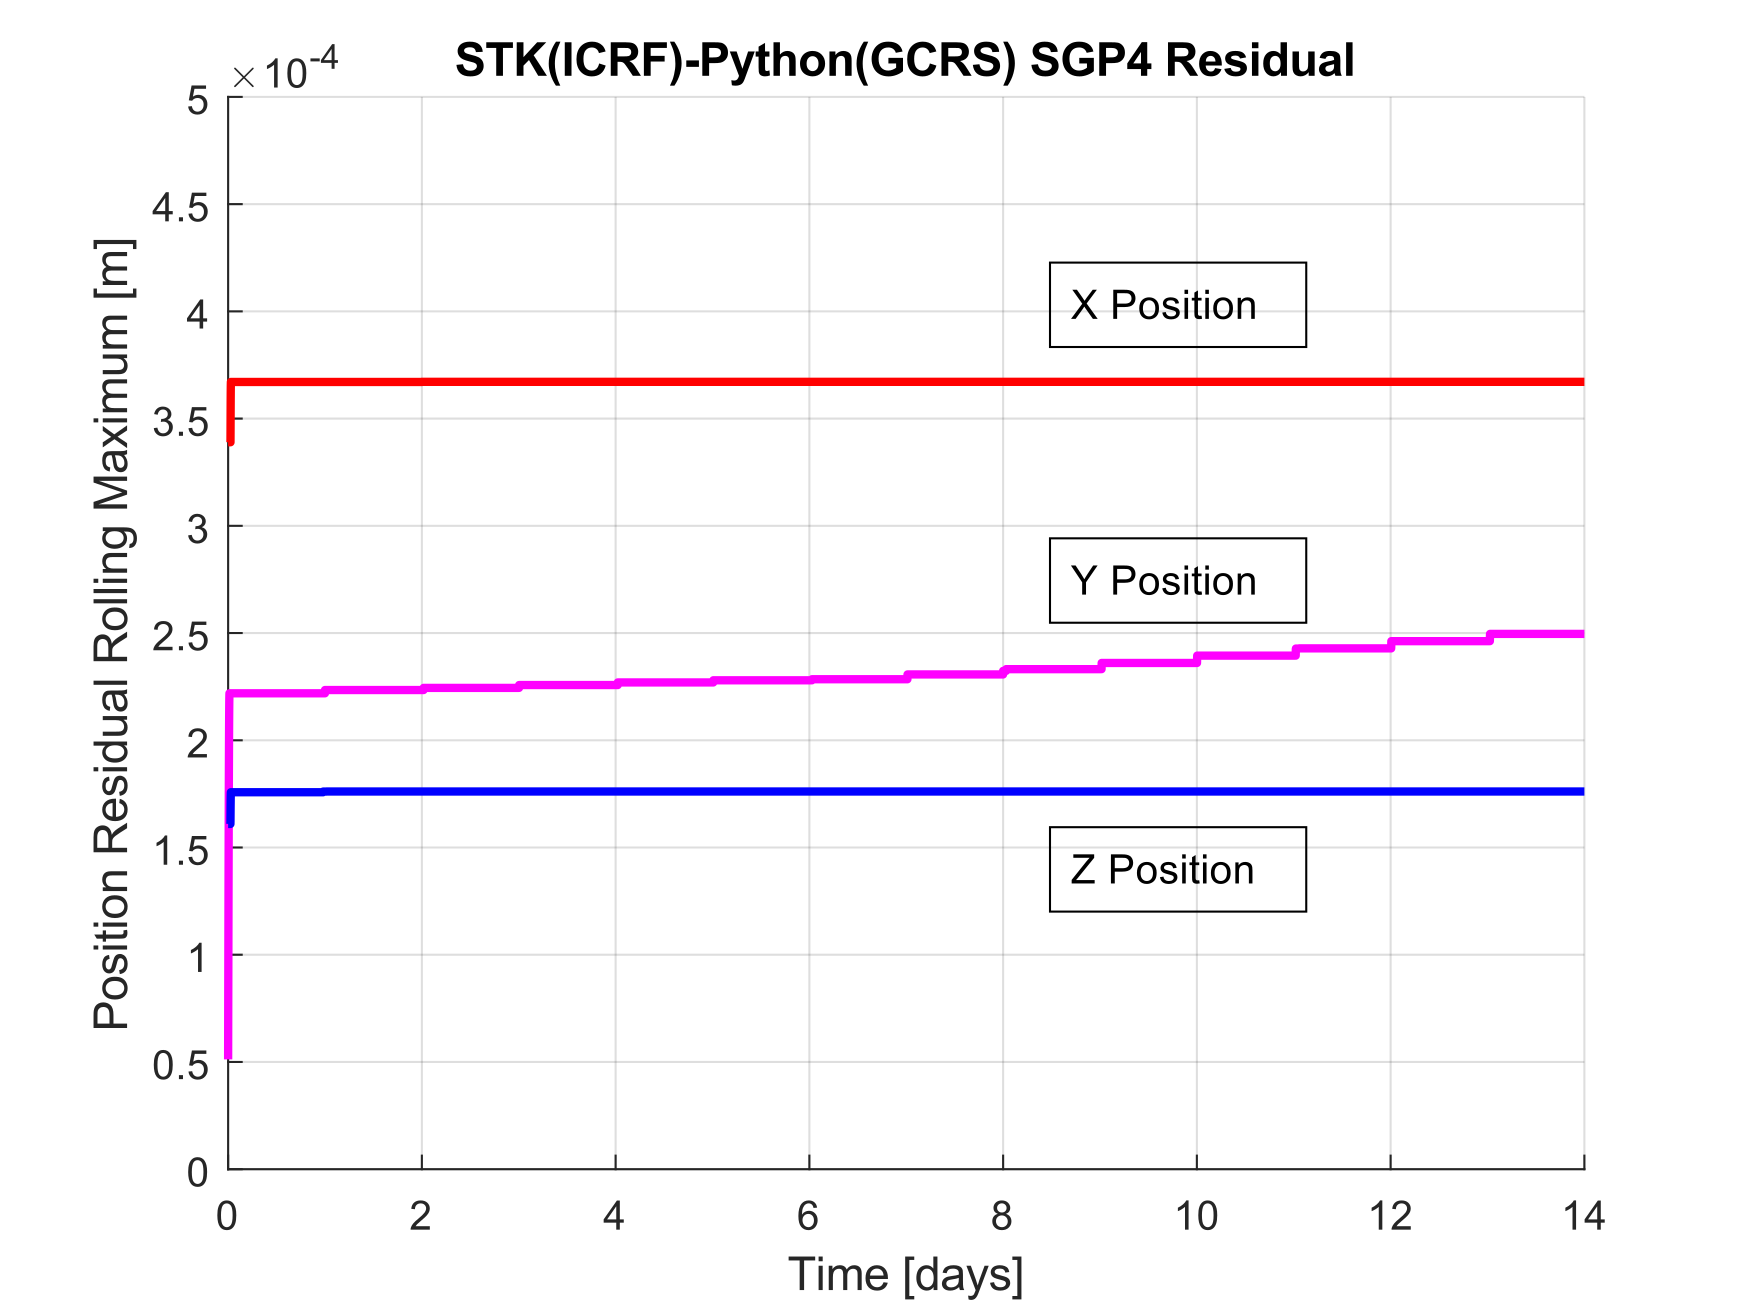
\includegraphics[width=0.7\textwidth]{STK_PY_residual-2.png} 
    \caption{Residual Difference \gls{stk} vs. Python}
    \label{fig:stk_py} 
\end{figure}

It is very easy to generate Ephemeris data. What is difficult is validating it.
The benchmark for validation is \gls{stk} since it has its own SGP4 ephemeris
generation capabilities. If operators did not use POPS, their best alternative
would be to set up scenarios manually in \gls{stk}. As such, using it as ground
truth is valid in this case. Both \gls{stk} and the \gls{pops} implementation
of SGP4 us the same source8: Revisiting Spacetrack Report \#39. As such, they
should provide the same results. One difference to note is that \gls{stk} uses
the \gls{icrf} \gls{eci} coordinate system but the propagator service uses
\gls{gcrf}.  This difference is acceptable since these reference frames are
approximately identical10. The procedure for validating the Propagator service
was first to select a \gls{tle}, a time range, a time step, and a coordinate
system.  Next was to generate Ephemerides from \gls{stk} and the propagation
service.  Finally, the results were compared. One such comparison can be seen
in Figure~\ref{fig:stk_py}. Here, the peak position residual was 0.37mm for the position along
the x-axis. The main purpose of this exercise is to ensure that the Python
libraries are being used correctly and that their output data is acceptable.
From this result, it is clear that the methods are identical and the difference
was most likely due to slight implementation differences. 

Another responsibility of the Propagator service is to determine a list of
passes for a given ephemeris. Having an entire ephemeris may be cumbersome for
some calculations so it makes sense to split a whole ephemeris into multiple
components. A `pass' is of course a completely general term so in this context
it is defined as the period between south-to-north hemisphere crossings as this
definition was chosen because it is easy to calculate an equator crossing. This
is where the z-position of a spacecraft goes from negative to positive.
\hl{See algorithm ?? for a discussion on how crossings are found}.

Part of the benefit of having the Propagator as its own service is that if a
more accurate algorithm is desired for orbital propagation, only the Propagator
service needs to be changed and the rest of \gls{pops} can be left as is.


%% ======================================================================== %%
%%			    Database
%% ======================================================================== %%

\section{Database}\label{sec:database}

\gls{pops} must be able to retain information, even if it is
shut down or moved somewhere else. It is also necessary that data be stored
such that it does not sit in \gls{ram}. For this reason, an \acrshort{sql}
database service is included with \gls{pops}. It stores all the data necessary
for \gls{pops} to function. This includes but is not limited to satellite
information, \glspl{tle}, current and previous plans, ephemeris data,
observation opportunity data, and planned observations. 

An \acrshort{sql} database is a type of database management system that uses
the \gls{sql}. It is commonly used where data needs to be organized and
accessed in a structured and efficient way. \gls{sql} is a programming language
used to manage and make changes to a \gls{rdbms}. In an \gls{rdbms}, data is
stored in tables with rows and columns. Using an SQL database allows for
effective data storage and access. Relationships may also be made with data in
an \gls{rdbms}. There are no read or write restrictions on an SQL database so
data can be accessed simultaneously by multiple users or services.

When a Docker container is deleted, all of the information stored in the
container is lost. To retain information between restarts, all of the data in
the database is stored in a Docker Volume. There are two ways information may
be persistently stored with Docker, either through bind-mounts or with Docker
volumes. Bind-mounts are simply just a directory on the host's system mounted
to the docker container. This is the simplest solution but it may be slow and
unreliable. Alternatively, with Docker volumes, the data is stored in Docker
itself. If Docker is deleted, so to is the volume. The benefit is that volumes
can be backed up and shared.

\begin{figure}
    \centering
    \includegraphics[width=0.8\textwidth]{database.png} 
    \caption{High Level Overview of the Database}
    \label{fig:database} 
\end{figure}

Figure~\ref{fig:database} shows a high-level overview of the structure of the
\gls{pops} database. The figure is not an exhaustive reference as some tables
have been omitted in favor of clarity. The entries in each table have also been
omitted for the same reason. While the figure may lack detail, it does give an
accurate qualitative description of the database's structure. 

Each box in the diagram represents a single table. Red boxes contain
`primitive' data. That is, data that has not been derived from any other
element. The blue boxes represent user-created data, or data that has been
created from user inputs. The green boxes represent raw data that has been
generated from \gls{pops}'s algorithms. Arrows indicate that there is a
relationship between two tables, including 1-to-1, 1-to-many, and many-to-many
relationships

Starting from the top, the base table for most \gls{pops} data is the
\textbf{Missions} table. \gls{pops} may be configured for other missions which
have different configurations. Each mission has a number of satellites stored
in the \textbf{Satellites} table. This table is a primitive because while
satellites come from a mission, they exist outside of \gls{pops} and cannot be
generated. They must be manually entered upon the creation of a new mission.
Each satellite will have multiple \glspl{tle}, stored in the \textbf{TLEs}
table. These may be pulled from online or custom generated.

Next is the most fundemental unit of mission planning, the \textbf{Plans}
table. A plan is derived from a mission and is associated with one \gls{tle}
for each satellite. Currently, plans are restricted to one set of \glspl{tle}.
If new \glspl{tle} are available, a new plan will need to be created. 

From a plan and its corresponding \glspl{tle} ephemerides are generated which
are stored in the \textbf{Ephemerides} table. This table only stores
information about the ephemeris, such as time range and step size. The actual
data is stored in the \textbf{Ephemeris Data}. The reason this information is
divided is such that information about an ephemeris can be queried without
having to load the entire table of data.

Another primitive table is the \textbf{Ground Stations} table. Here information
is stored for each ground station, such as Latitude, Longitude, Altitude,
Elevation Mask, etc. From satellite ephemerides, we can generate \textbf{Ground
Access Times} using the Ground Access Utility from the \glspl{atu}.

Areas of Interest may be stored in the \textbf{AOIs} table. These may be
generated from a file or drawn by a User. The data for each \gls{aoi}, is
generally stored as a JSON string, which can be parsed when requested.

From a plan and an \gls{aoi} we may search for opportunities through a
\textbf{Search Scenario}.  This table contains information about what kind of
search was performed, as well as what configuration parameters were included.

Not all satellites may be included in a search scenario. To capture this
information, there is a \textbf{Search Satellites} table which links search
scenarios with satellites and search data.

Depending on the type of search, raw search data may be stored in the,
\textbf{Access Times}, \textbf{Swaths}, and \textbf{Intersection Polygons}
tables. Each data point is associated with a search satellite. 

Lastly, at the end of the search hierarchy is the \textbf{Opportunities} table.
This table is simply a list of references to raw search data. With just the raw
search data, determining what constitutes an `opportunity' may indeterminable.
So when the search data is generated, so to is the corresponding opportunity

Separate from the rest of the tables discussed so far is the \textbf{Schedule}
table. Here Events are stored. Each Event is linked to a satellite, and may
also be linked to a plan.

It should be noted that the Database service only hosts the \gls{sql} database.
To interact with the data, either the \acrshort{orm} in the Mission Model
service must be used or a separate database viewer.



%% ======================================================================== %%
%%			    ATUs
%% ======================================================================== %%

\section{Access Time Utilities}\label{sec:atu}

The ATU service provides the basic building blocks for
constraining observation opportunities. These can be added to depending on a
mission’s need. Some utilities the \gls{atu} service currently supports are
calculating: ground station access times, swath generation, and polygon
intersection with a swath. We will not go too much into detail on how some of
these are calculated but rather we will discuss how they are used at a
\gls{pops} level.

\subsection{Ground Access Utility}

A \textit{ground access} is defined as the time interval during which a
satellite can establish contact with a ground station. A \textit{ground
station} is a point on the Earth’s surface, identified with geodetic
Latitude-Longitude-Altitude coordinates and an elevation mask. An
\textit{elevation mask} is the angle above the horizon, at the ground station’s
position, at which the satellite can be considered visible by the ground
station. Calculating the ground access for satellites on a mission is a
fundamental task in operations planning. These time intervals dictate the
opportunities for data downlink, command uplink, and any other communication
between the ground segment and satellite.

The simplest way to compute ground access involves propagating the orbit of a
satellite and checking, at every time step, the position of the satellite
relative to the ground station and testing whether the relative position is
above the elevation mask. While this method is trustworthy and capable of
returning accurate results, its reliance on iterating over an entire satellite
orbit input typically yields a long runtime. This is particularly evident in
the case where a mission has multiple ground stations, multiple satellites, or
a short propagator timestep. The computation time drawback motivates the use of
other algorithms that can determine ground access more efficiently.

\begin{figure}[h]
    \centering
    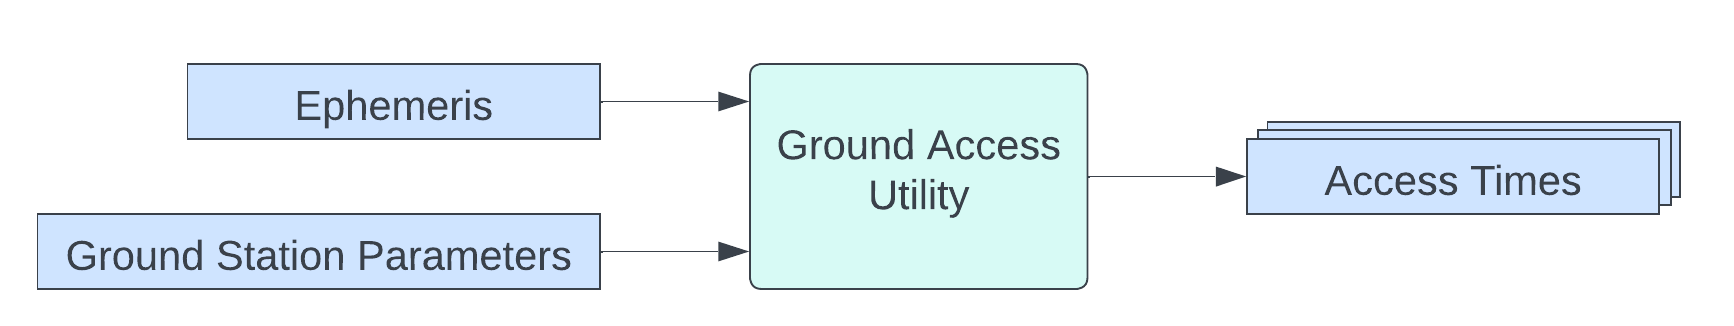
\includegraphics[width=0.7\textwidth]{ATU-1.png} 
    \caption{Input Output Diagram for Ground Access Utiltiy}
    \label{fig:atu-1} 
\end{figure}

So, from a satellite ephemeris and some ground station information, the access
time utilities will generate a list of Access Times. That is the \textit{time}
of an access and the \textit{type} (access enter or access leave) of an access
will be specified. This is illustrated in Figure~\ref{fig:atu-1}.

\subsection {Swath Utility}

\begin{figure}
    \centering
    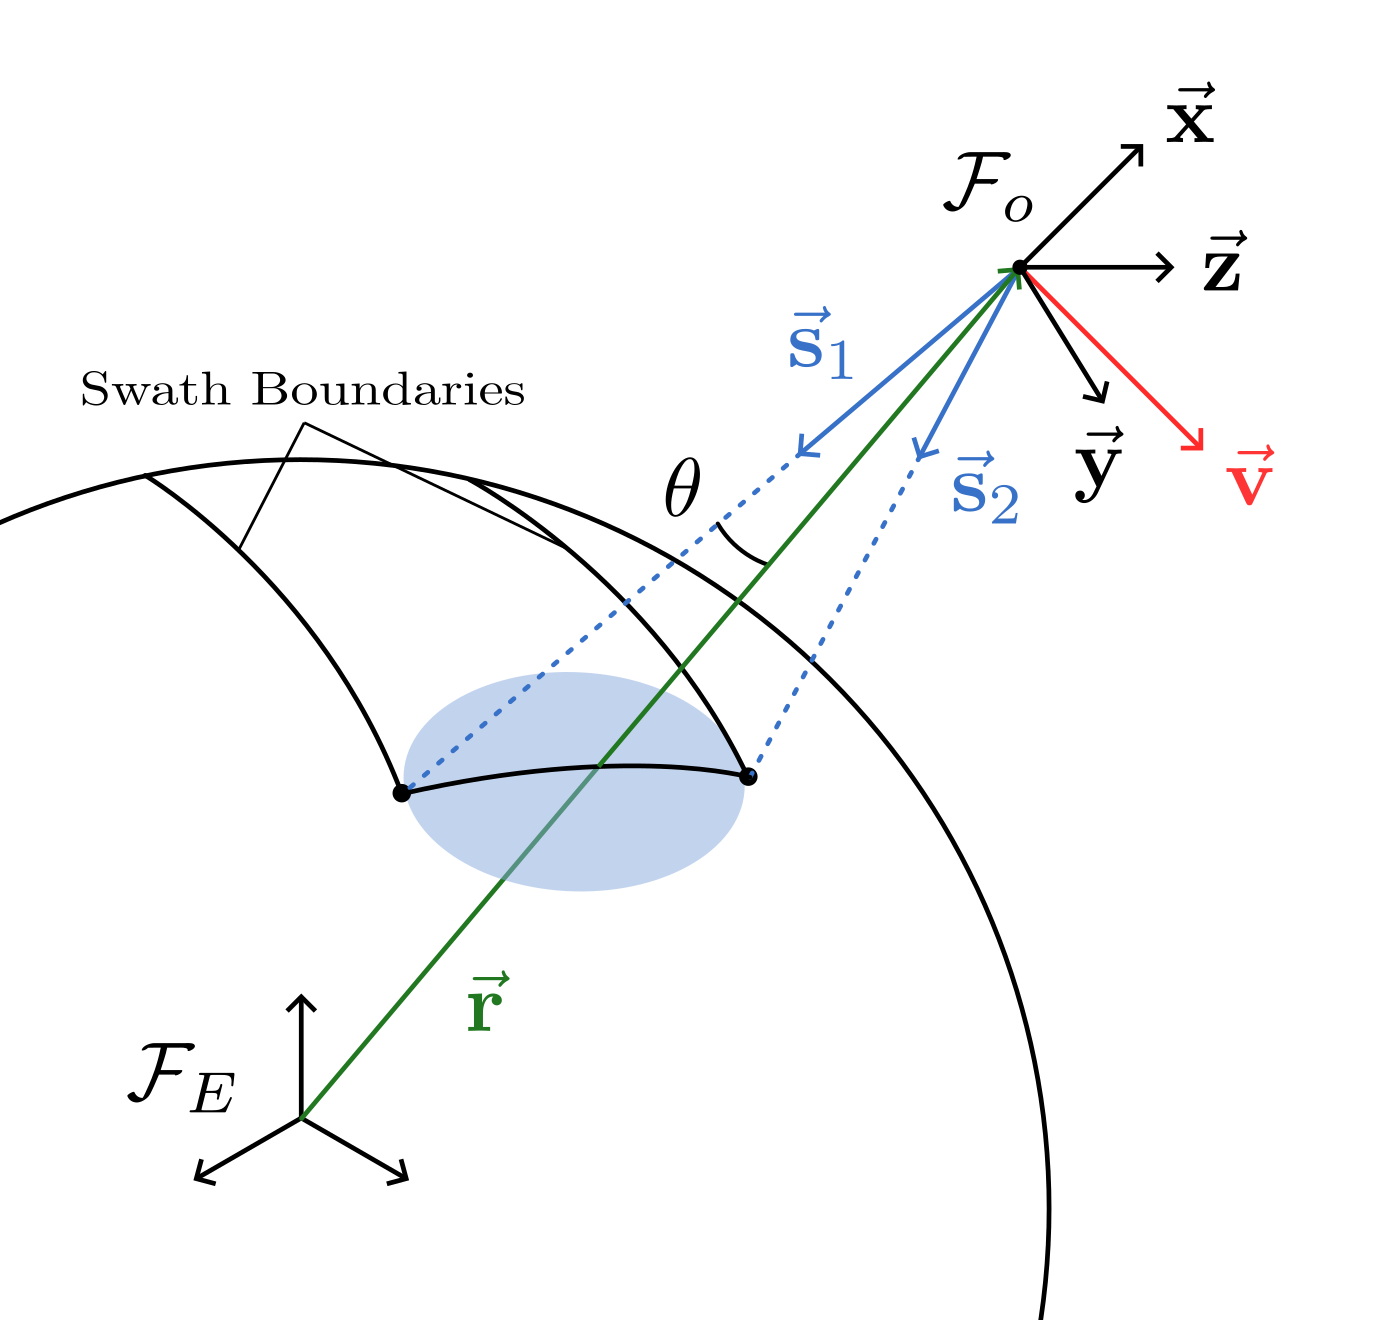
\includegraphics[width=0.5\textwidth]{Swath Bound.png} 
    \caption{Access Swath Boundary Calculation}
    \label{fig:swath-bound} 
\end{figure}

As discussed in the Terminology section, the concept of an access swath is
defined as a time-series of access regions as a satellite orbits the Earth.
Within \gls{pops}, a swath is represented through a closed curve that describes
the boundary of the cumulative access region of a sensor’s \gls{for} over a
time interval. The process for calculating a swath boundary from an input
ephemeris is described here.  

\newcommand{\Fo}{$\vec{\mathcal{F}}_o$} 
\newcommand{\Fe}{$\vec{\mathcal{F}}_E$}

Let us first define the orbital reference frame of the satellite, \Fo, with
respect to an ECEF fixed coordinate system, \Fe,  Then, let us take the
satellites position, $\sev{r}$, and velocity, $\sev{v}$, with respect to \Fe.
These two vectors are given for a single epoch in an ephemeris file. \Fo ~is
then defined as $ \vec{\mathcal{F}}_o = \left[ \sev{x}, \, \sev{y}, \, \sev{z}
\, \right]^T$, where:

\begin{equation} 
    \sev{x} = \frac{\sev{r}}{\norm{\sev{r}}}, 
    \quad 
    \sev{z} = \frac{\sev{r}\times\sev{v}}{\norm{\sev{r}\times\sev{v}}}
\end{equation}

And lastly $\sev{y} = \sev{z} \times \sev{x}$ to form an orthonormal set, but
this is not important for our purposes. We shall then take two vectors,
$\sesv{s}{1}$ and $\sesv{s}{2}$, that form the boundary of our conical FOR and
lie within the x-z plane of \Fo,  These are defined as,

\begin{align}
    \sesv{s}{1} &= \vec{\mathcal{F}}_o^T \left[ \, -\cos\theta, \quad 0, \quad -\sin\theta \right]^T \\
    \sesv{s}{2} &= \vec{\mathcal{F}}_o^T \left[ \, -\cos\theta, \quad 0, \quad \sin\theta \right]^T
\end{align}

Where $\theta$ is the half-angle of the satellite’s \gls{for}. These vectors
are then transformed to \Fe~and the points where they intersect the Earth’s
service are the swath’s bounds for that time instant. If this calculation is
performed multiple times and the boundary points are connected, two lines are
formed on the Earth’s surface. These lines are the satellite’s swath boundary
for that time range.  This process is illustrated in
Figure~\ref{fig:swath-boundary}.

Using the same process, we may also find the ground track of the satellite by
using the nadir vector, $\sesv{s}{n}$, which is defined as:

\begin{align}
    \sesv{s}{n} &= \vec{\mathcal{F}}_o^T \left[ 1, \quad 0, \quad 0 \right]^T
\end{align}

\newcommand{\Cx}[1]{\ses{C}{x}\!\!\left(#1 \right)}

Lastly, we may also approximate the access region for each timestep. To do so,
we can take an off angle vector, $\sesv{s}{1}$, and rotate it around the
x-axis. Where the vector intersects the Earth's surface will be a boundary
point of the access region. For $N$ boundary points, we must rotate the vector
$N$ times. Let us first define a rotation matrix about the x-axis of \Fo~for
some angle, $\phi$:

\begin{equation}
    \Cx{\phi} = 
    \left[
	\begin{array}{ccc}
	1  & 0 & 0   \\
	0 & \cos\phi  & -\sin\phi   \\
	0 & \sin\phi  & \cos\phi
    \end{array}
    \right]
\end{equation}

We may then generate the set of vectors, $S$, that describe the \gls{for} for
that time instant:

\begin{equation}
    S = \in  \left\{ \Cx{2\pi/n} \sesv{s}{1} \, \vert \, n = 1, 2, \ldots N \right\}
\end{equation}
Typically, access regions are described with 8 points but more can be added if
necessary. 


\begin{figure}[h]
    \centering
    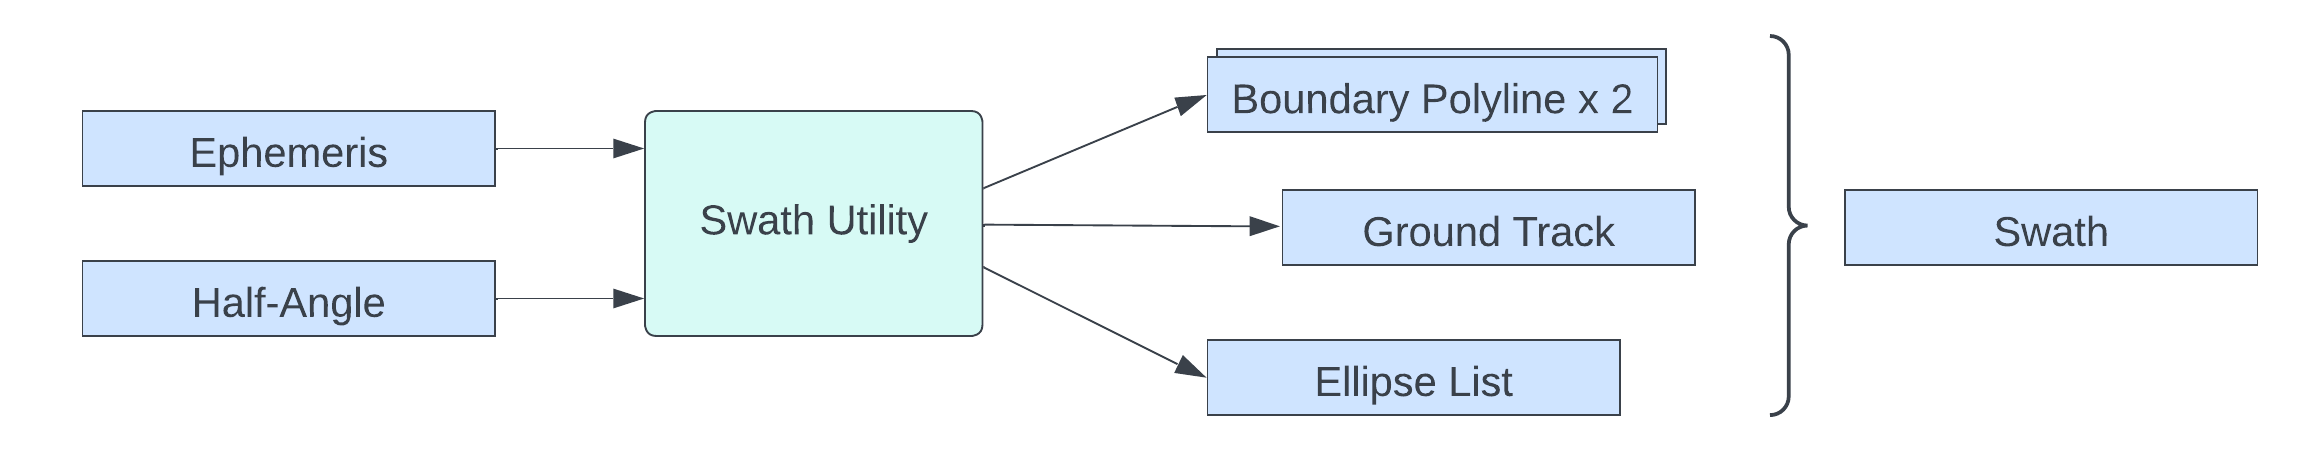
\includegraphics[width=0.7\textwidth]{ATU-2.png} 
    \caption{Input Output Diagram for Swath Utility}
    \label{fig:atu-2} 
\end{figure}

In summary, for every ephemeris point, a swath boundary is calculated, a a
ground track is calculated, and a list of ellipses (access regions) are
provided. This can be seen in Figure~\ref{atu-2}


\subsection{ Swath Intersection Utility }

Swath intersection is an important operation for determining what part of a
specified region is observable by a satellite sensor during some time interval.
Regions are polygons on the Earth’s surface whose vertices are oriented
counter-clockwise. The edge between two consecutive vertices is the great
ellipse arc connecting both points. Swaths are also approximated as polygons
provided that the timestep is small enough. The edge between two swath boundary
points being a great ellipse arc is assumed to be a sufficient approximation.

Polygon clipping techniques are used to find the area of intersection between a
swath and a polygon. First, the swath and polygon vertices are transformed into
2D coordinates. The 2D projection used involves defining a plane that is
tangent to some point on the Earth’s surface.  To project a point on the
Earth’s surface to this plane, a vector is drawn from the centre of the Earth
towards the point (its ECEF coordinates), and the vector is extended towards
the point of intersection of the plane. This type of projection is commonly
known as the Gnonomic projection; its advantage with respect to the polygon
clipping operation is that great ellipse arcs are projected as straight lines.
This means classical 2D polygon clipping techniques can be applied to polygons
drawn on the Earth’s surface. So long as the swath and polygon occupy one
hemisphere of the Earth’s surface, the projection will accurately represent the
points of intersection of the swath and polygon, and any polygon clipping
technique can be applied.


\begin{figure}[h]
    \centering
    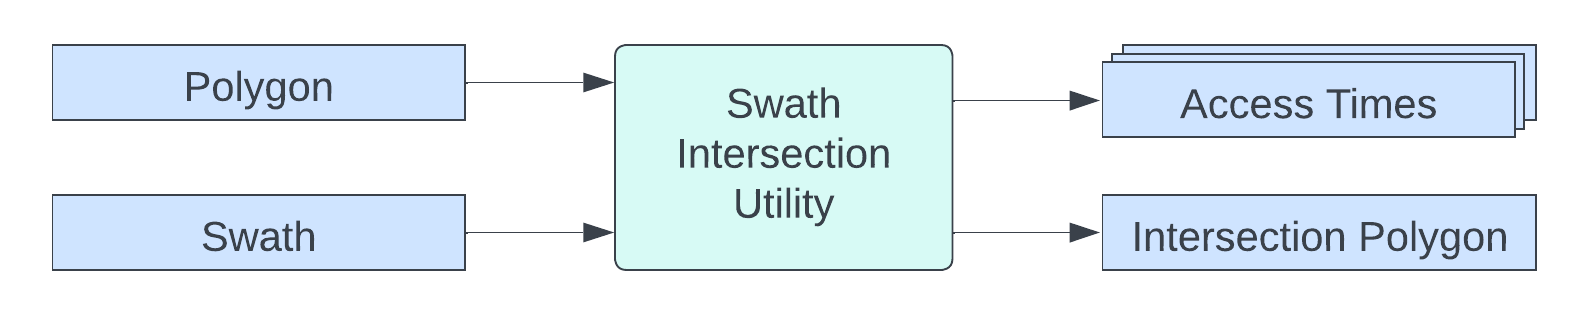
\includegraphics[width=0.7\textwidth]{ATU-3.png} 
    \caption{Input Output Diagram for Swath Intersection Utility}
    \label{fig:atu-3} 
\end{figure}

So given some swath data, specifically the swath boundaries and ellipse list,
the Swath Intersect Utility will return a list of access times and an
intersection polygon between the swath and the polygon. This is illustrated in
Figure~\ref{fig:atu-3}

%% ======================================================================== %%
%%			    Mission Model
%% ======================================================================== %%

\section{Mission Model}
 
The Mission Model service is the service that contains the main logic for most
of \gls{pops}'s functionality and front-end \gls{gui}. When a user interacts
with \gls{pops}, they are interacting with the Mission Model service. As such,
it is quite large and has a number of responsibilities. Some of them are:

\begin{outline} 
    \1 Database management,
    \1 Displaying an interactable front-End User Interface,
    \1 Earth Visualization,
    \1 Plan Configuration, and
    \1 Scheduling.
\end{outline}


\begin{figure}[h]
    \centering
    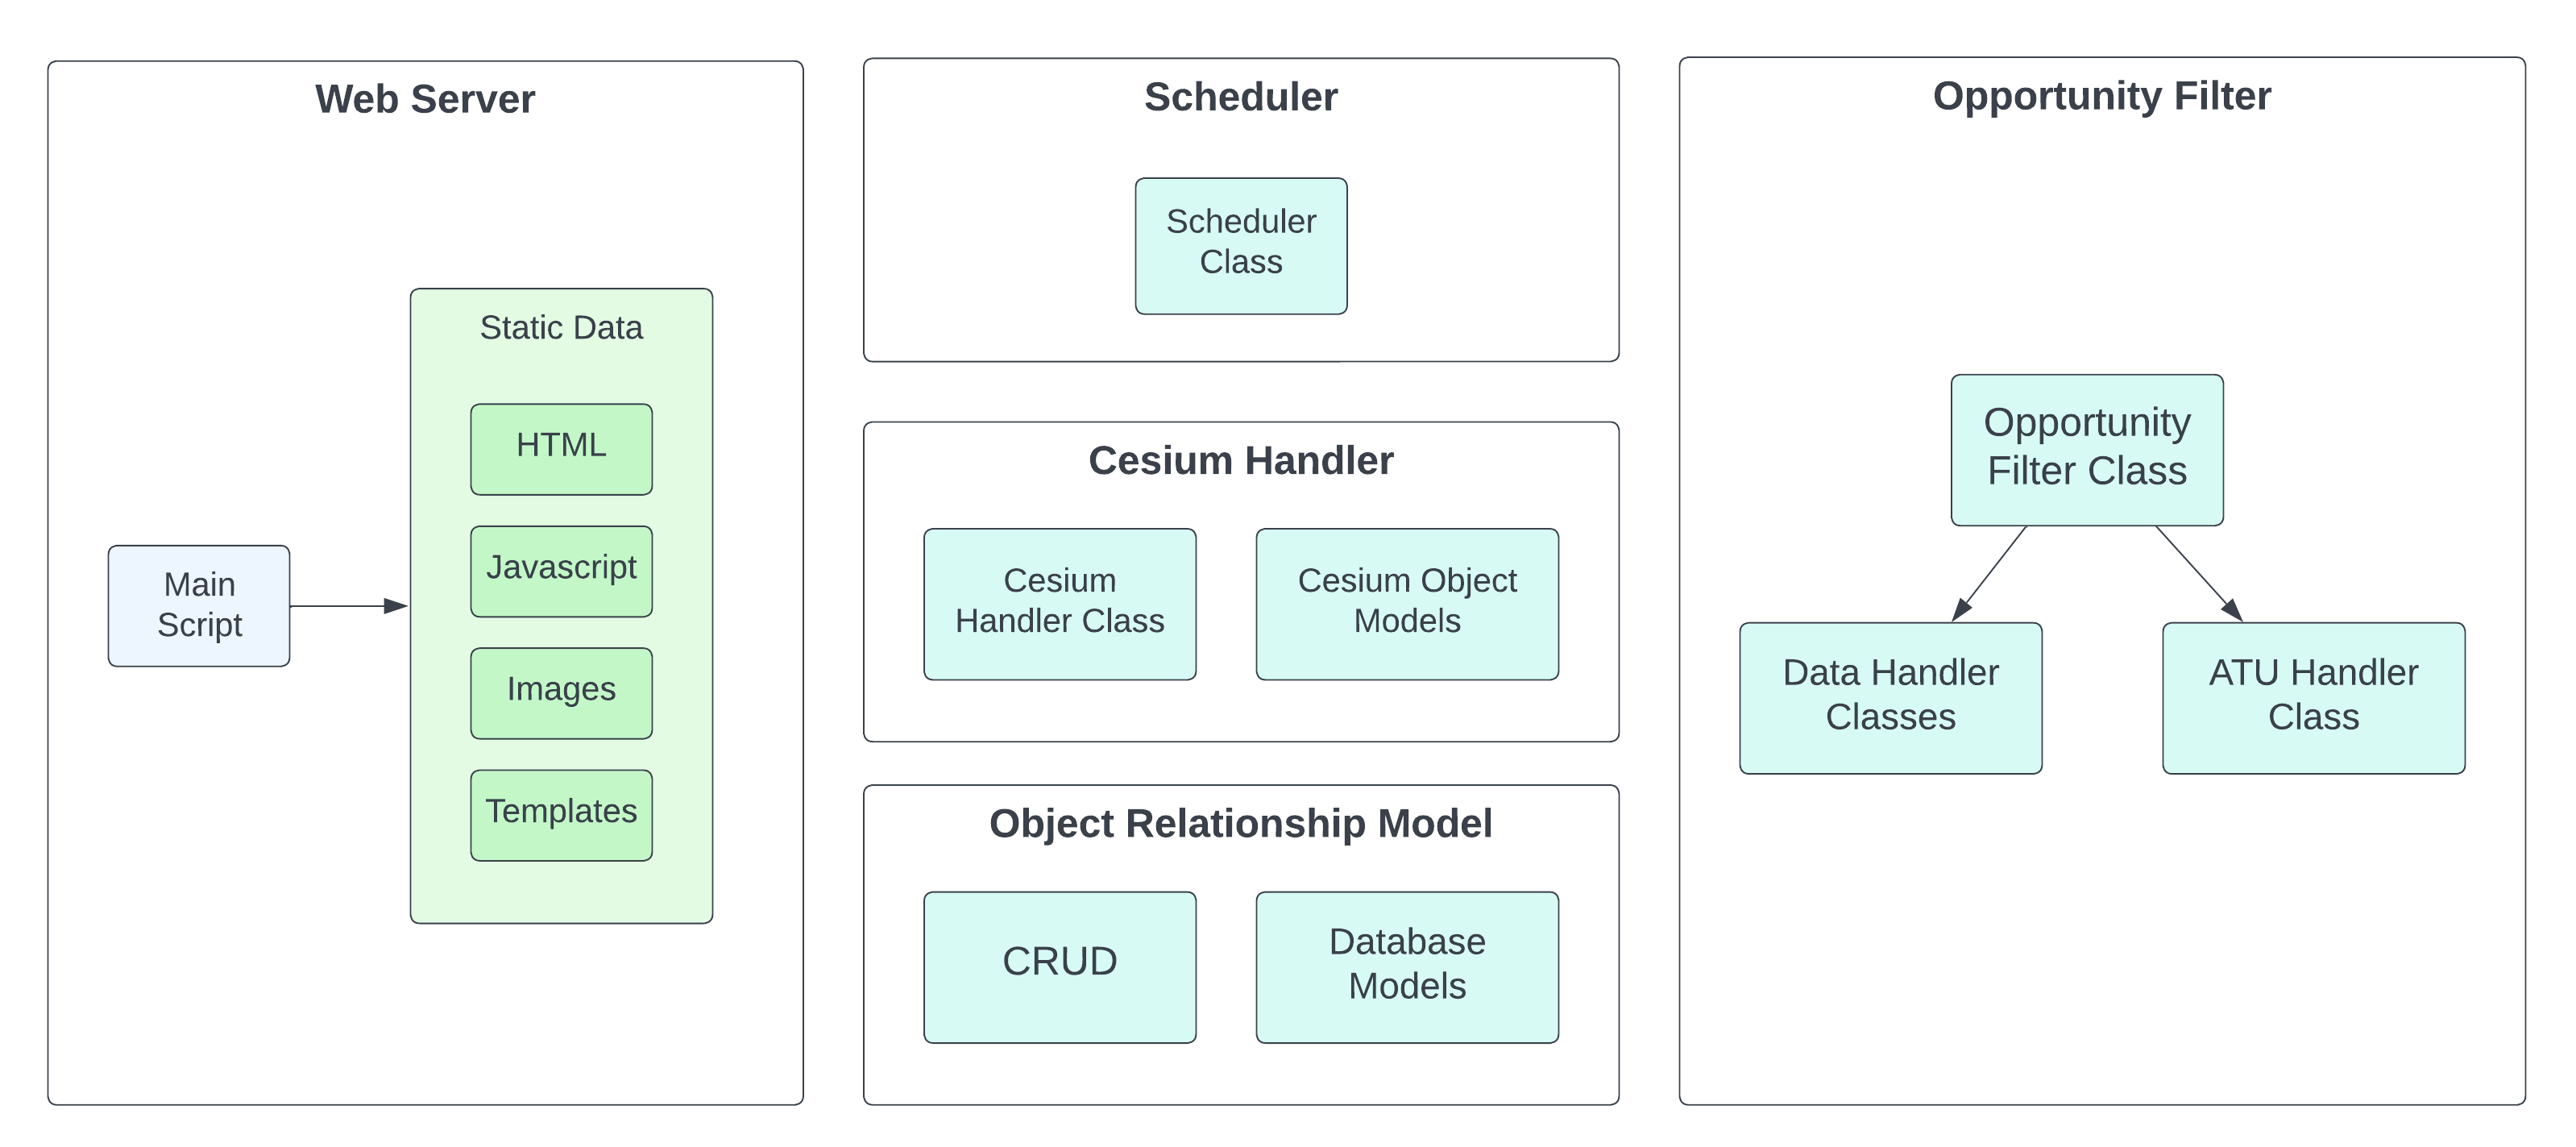
\includegraphics[width=0.7\textwidth]{Mission Model.png} 
    \caption{High Level Structure of Mission Model Service}
    \label{fig:mission_model} 
\end{figure}

A high-level overview of the Mission Model service can be seen in
Figure~\ref{fig:mission_model}. There are many components but we will go
through them one by one.

\subsection{Main} 

The main Python script acts as the base for the entire Mission Model service.
Its purpose is to, among other things, set up the web server, load environment
variables, instantiate the handler classes, and associate API calls with their
callback functions. Setting up the web server is the same as with any other
service. The environment variables range from server metadata to addresses of
other containers. There are a number of utility classes that handle various
aspects of \gls{pops}. These are the: scheduler, \gls{atu} handler, data
handler, and opportunity filter classes. They will be discussed in the
following sections. The most important part of the main service is defining API
calls. If a user wishes to interact with \gls{pops}, they must enter a link on
the their browser, that information is then sent to the web server, and a
callback function in the Mission Model service is called. It is the Mission
Models responsibility to consolidate information, whether that be from the
database, through HTML templates, or new information that must be calculated.
The Mission Model service does very few actual calcualtions, its only purpose
is to organize information and call functions as necessary to serve a request.
Currently, the main service is large and difficult to navigate because of its
size. In the future, it will be refactored to a number of sub-scripts that
handle specific functionality in the service.

\subsection{Object Relationship Mapping}

The Database is its own service but the Mission Model is currently the only
service that interacts with it. It does so by using an \gls{orm}. An \gls{orm}
is a method of modeling a relational database through an object-oriented
language. For our purposes, the \gls{orm} serves two functions, it describes
how the data is being stored in the database and it describes how we can
interact with the database programmatically. For \gls{pops}, we are using an
open-source \gls{orm} library. It handles the low-level functionality and
allows us to focus on what is unique about \gls{pops} rather than databases in
general. For example, there is no need to develop our own methods of
formulating \gls{sql} queries or parsing the ouptut data once it is retrieved. 

To set up the \gls{orm} for \gls{pops} we need at least two scrips, a models
file and a \gls{crud} file. The models file defines explicitely how tables are
layed out in the database through Python classes. Information such as: what
tables there are, what columns are in each table, what keys are included with a
table, and what relationships there are between tables. If a change is made to
the database, it must be reflected manually in the models file and vice-versa.
The \gls{crud} file, as its name suggests, allows us to interact the database.
It is a library of functions that allows a developer to formulate \gls{sql}
queries at a high level with Python syntax. The \gls{crud} file also relies on
the classes from the models file to refer to tables. For example, if we wished
to retrieve a satellite with a particular id from the \texttt{Satellites}
table, we would create a new function in the crud file with a descriptive name
such as \texttt{get\_satellite\_by\_id(sat\_id)}. Within this function we would
construct a query that searches the \texttt{Satellites} table for a row whose
id column, \texttt{Satellites.id}, matches the input id, \texttt{sat\_id}. The
\gls{orm} gives a developer a great deal of flexibility when formulating
queries or inputting data and makes interacting with the database easy to
understand and easy to expand.


\subsection{Static Data}

For the webserver to function there is a large amount of static data that must
be stored on the server and that must be retrieved when necessary. This may be
\gls{html} files, \gls{html} templates, JavaScript files, \gls{css}
stylesheets, and images.

Webpages are not generated completely programmatically. Either the \gls{html}
for these pages are written in advance and loaded directly upon being requested
or, they are assembled from HTML templates and configured depending on input
parameters given by the user or by what data is available at that time. Writing
out the HTML for a webpage in its entirety is acceptable for situations where
nothing changes on the webpage and everything should be left as is. This is the
case for high-level menus and settings pages. If anyhting else is required,
\gls{html} templates should be used. HTML templates allow for a great deal of
configurability when loading webpages. They can range from simple text
replacement to loading other templates. Some template engines even allow for
some programmatic features within the template itself such as looping, if/else
statements, or even custom functions.

Generally, as a design decision, as much of the underlying logic for \gls{pops}
has been limited to Python. The main reason for this is to consolidate the
logic to one language. Unfortunately for web development, Javascript and
\gls{css} are unavoidable and must be used as necessary. When they are used
they can be added directly to an HTML document or template but this is
generally not the best way. Having different scripts or different styles placed
haphazardly in the codebase gets messy quickly and may lead to code duplication
or even conflicting functions. To combat this, JavaScript and \gls{css} files
are stored separately and then statically referenced in the \gls{html} file
they apply to. By consolidating these files, it is much easier to organize and
reference them as necessary. 


\subsection{Data Handlers}\label{sec:data_handler}

For \gls{pops}, there is a great deal of data and many different ways that the
data can be formatted in. In an attempt to generalize the data and make it
easier for a developer to work with, several Data Handler classes have been
created to handle data format conversions and to provide helper functions. The
differences in data formats can be as simple as differences in what keys are
used in dictionaries of key-value pairs. For example, the Propagator service
uses the key \texttt{`position'} and the \glspl{atu} use the key
\texttt{`pos'}.  This is a small discrepency and if all the differences were
this simple, then we would just set some standard data format and be done with
it.  Unfortunately, there are larger differences that require conversion. When
describing lists of points there are currently 3 different formats. The
Propagator service generates a list of points, $P_1$, as a list of the x, y,
and z components for all $N$ points. 

\begin{align*}
    P_1 &= [\se{x}, \se{y}, \se{z}] 
\end{align*}
where
\begin{align*}
    \se{x} &= [x_0, x_1, x_2, \ldots, x_N],  \\
    \se{y} &= [y_0, y_1, y_2, \ldots, y_N],  \\
    \se{z} &= [z_0, z_1, z_2, \ldots, z_N]
\end{align*}

To describe swath boundaries as lists of points, $P_2$, the \gls{atu} service
uses a dictionary of key-value pairs. There is one string key for each
component (\texttt{`x'}, \texttt{`y'}, and \texttt{`z'}) and the value for each
is the list of components for all $N$ points. 

\begin{equation*}
    P_2 = 
    \left\{
    \begin{aligned}
	\texttt{`x'}&: [x_0, x_1, x_2, \ldots, x_N],  \\
	\texttt{`y'}&: [y_0, y_1, y_2, \ldots, y_N],  \\
	\texttt{`z'}&: [z_0, z_1, z_2, \ldots, z_N]
    \end{aligned}
    \right.
\end{equation*}

Lastly, the graphical Earth Visualization tool Cesium expects lists of
points,$P_3$, to just be a single list, where the components of each point are
ordered one after the other.

\begin{equation*}
    P_3 = \left[ x_0, y_0, z_0, x_1, y_1, z_1, \ldots x_N, y_N, z_N \right]
\end{equation*}

All of these formats contain the same information but organized in different
ways.  A developer should not have to write conversions everywhere whenever
they wish to use a data type.  They should only have to worry about the data
itself and not how it needs to conform with whatever format. It is for this
reason we must consolidate these conversions in separate data handler classes.
Of course, there is much more data and many more data formats that must be
supported, but these three examples are sufficient to give the reader an idea
about the nuances involved. There are many Data Handler classes but the
following are some of the larger more important ones.


\subsubsection{Ephemeris Data Handler}

Ephemerides are the most important collections of data as they are used as a
basis to calculate most other data. As such, they are referenced many times and
have a number of different formats. There are four different areas where
Ephemerides are referenced: the Propagator service, the \gls{atu} service, the
Cesium Viewer, and the Database. An Ephemeris object contains some of the
following information:

\begin{description}

    \item[Epoch] An ISO 8601 Datetime string in UTC specifies the reference
	time for the ephemeris data.

    \item[Seconds] An array of float values that specify the offset from the
	epoch.

    \item[Position] Position vectors of the satellite. Each corresponds to a
	seconds offset.

    \item[Velocity] Velocity vectors of the satellite. 

    \item[Pass Index] For each ephemeris point, the pass index is specified. 

\end{description}


An Ephemeris object can either be created by sending a request to the
Propagator service or it can be loaded from the Database. For the case where we
generate a new ephemeris from the Propagator service, the Ephemeris class
handles communication with the Propagation service and directly saves the
ouputted ephemeris data into a private variable. The propagator ephemeris data
format serves as the base format from which we can convert to other formats as
necessary. For example, there are member functions that take the saved
ephemeris data and converts it into the format expceted by the \glspl{atu} or
into a format expected by Cesium. Alternatively, if an ephemeris is loaded from
the database, each row must be sorted, processed, and converted to the base
format. 

In some scenarios we do not wish to work with an entire Ephemeris for a large
scenario, rather we may wish to only consider a subset of a larger Ephemeris
object. When we take a subset of a larger Ephemeris, we refer to this process
as `constraining' the Ephemeris. For this, a helper function has been added
which accepts a time range that lies within the time range the Ephemreis object
is defined for. This helper function then generates a new Ephemeris object
which only contains the ephemeris data that lies in the desired time range.  

\subsubsection{Swath Data Handler}

The Swath Data Handler classes behaves very similarly to the Ephemeris Data
handler. It too must have data conversion methods for the \glspl{atu}, for
storage and retrieval from the database, and for loading into Cesium. It also
has a helper function that constrains the Swath object to a specified time
range. 

It should be noted that at this level, there is no distinction between an
access swath and a ground swath. Both are generated in the same way, stored in
the same way, and displayed in the same way. Whether they are defined based on
a \gls{fov} or \gls{for} is immaterial and not relevant in this context. 

The data a Swath object stores is similar to an Ephemeris object. It
also has an epoch and a seconds array. These match the epoch and seconds array
of the Ephemeris object the Swath object was generated from. It also contains
data that is unique to Swaths:

\begin{description} 

    \item[FOV/FOR] For reference the FOV or FOR angle is stored along with the
	swath data.

    \item[OFF-1/2] These are the boundary polylines of the Swath object. They
	are stored as lists of points.

    \item[Ground Track] For display purposes, it may be useful to display the
	ground track of the satellite generating the Swath Object so this
	information is stored as a list of points.

    \item[Ellipse List] Each swath timestep in a Swath Object is also given an
	Ellipse. See section\ref{sec:atu-ellipse}.

\end{description}


\subsubsection{Polygon Data Handler}

The Polygon Data Handler is the last data handler class of note. It is used to
represent area target \glspl{aoi} or intersection polygons. The core data a
Polygon object contains is simply just a single list of points.  As with the
Ephemeris and Swath data handlers, there is a small sweet of data format
conversions.  But, for the Polygon Data Handler, much of the funcitonality lies
in its utility functions.

The first utility function is simple; it merely transforms all of the points in
the Polygon from \acrfull{ecef} cartesian-xyz coordinates to
Latitude-Longitude-Altitude coordinates and vice-versa.  Generally, with other
objects such as Ephemeris objects or Swath objects, their underlying datawill
never be explicitly displayed to the user. For this reason, points in those
objects can be left as cartesian coordinates. But, when a user creates a
Polygon object or if the coordinates of the vertices need to be displayed to
the user, Latitude and Longitude is much more human readable than cartesian
coordinates. 

Early on in development, there were some restrictions placed on the types of
polygons that the \glspl{atu} could accept. One restriction was that polygons
must be convex. That is for the set of all points that lie within a polygon,
there do not exist two points such that if a line is drawn between the points,
that line intersects with an edge of the polygon. At first, it seemed as though
this only limited the types of area-targets that could be specified but through
developing the opportunity filter class there arose some scenarios where
concave polygons were generated that needed to be inputted into the
\glspl{atu}. For this reason, a simple algorithm was implemented that removes
vertices to force a poygon to be convex. The implementation for this is
discussed in Algorithm~\ref{alg:force-convex}. Thankfully, this restriction has
been lifted but the implementation is interesting nonetheless.

Another restriction placed on polygons is that their vertices must be ordered
counter-clockwise (the motivation for this is discussed in
Section~\ref{sec:cesium-models}). If a polygon is ordered in a different way,
this may lead to garbled results from the \glspl{atu} or Cesium viewer. If
necessary, when generating a Polygon object and a developer suspects that the
source data may be un-ordered, they may set an option to \textit{force} a
polygon to be counter-clockwise. Re-ordering is not always perfect, though, and
that is why this is an option and not always done. The implementation for this
can be found in Algorithm~\ref{alg:ccw}.


 

\subsubsection{Other Data Handlers}

There are a number of other data handler classes that are used but don't have
as noteable functionality. Some of these are:

\begin{itemize} 
    
    \item Access Times Data Handler
    \item Ground Station Data Handler
    \item Sensor Data Handler

\end{itemize}

For the Access Times Data Handler, there exists one utility function. There are
some situations where a developer may need to determine what access times, if
any, lie within some defined period of time. For this the Single Access
Intersection algorithm was developed which is discussed in
Algorithm~\ref{alg:contains}.


\subsection{Access Time Utilities Handler}

In order to abstract the communication between the Mission Model service and
the \gls{atu} service, an \gls{atu} handler class has been developed. Its
purpose is simple, from input data data, it sends requests to the \gls{atu}
service and formats the result. A developer shouldn't need to create a POST
request every time they wish to utilitize some \gls{atu} functionality. They
may make a mistake that wastes development. 

Every \gls{api} call provided by the \gls{atu} service has a corresponding
method in the \gls{atu} handler. For ease of use, the inputs and outputs of
each method are Data Handler objects. For example, if a user wishes to perform
polygon intersection with a swath and a polygon, all they must do is pass a
Swath object and Polygon object to the \texttt{polygon\_intersection()} method
and an Access Times object and another Polygon object will be returned. The
purpose of this is to make interacting with the \gls{atu} service as simple as
specifying their high-level inputs and outputs.


\subsection{Opportunity Filter}

The Opportunity Filter class is the most important but also most complex aspect
of the Mission Model service. It is here that the Mission Model actually
searches for potential observation opportunities and implements the filters
discussed in Section~\ref{sec:opp-filtering}. Its purpose is to combine
the functionality of the Data Handler classes and the \gls{atu} Handler class
to make Opportunity Filtering as close as possible to their high-level
summaries. In general, with opportunity filtering, the implementation process
is straightforward and matches well with its high-level description. This is
not always the case though. Let us now revisit the Filters discussed earlier,
and outline how they are actually implemented in \gls{pops}. 

\algnewcommand\algorithmicforeach{\textbf{for each}}
\algdef{S}[FOR]{ForEach}[1]{\algorithmicforeach\ #1\ \algorithmicdo}

\begin{algorithm} 
    \caption{Coarse Imaging Opportunity Filter}
    \label{alg:coarse-imaging} 
    \begin{algorithmic}[1]
	\Function{CoarseImaging}{$E_A$, $g_{AOI}$} 

	    \Let{$S_A$}{\Call{Swath}{$E_A$, $60^\circ$}} \Comment{Coarse Imaging Swath}

	    \Let{$A_{A}$, $G_A$}{\Call{PolygonIntersection}{$S_A$, $g_{AOI}$}} 

	    \Let{$O$}{$[A_{A}, G_A]$} \Comment{List of Opportunities}
	\State \Return $O$, $S_A$
	\EndFunction
    \end{algorithmic}
\end{algorithm}

The implementation of the Coarse Filter can be seen in
Algorithm~\ref{alg:coarse-imaging} and is very close to its high-level
description. The inputs to the filter are the Ephemeris of Sat-A, $E_A$, and
the Area of Interest polygon $g_{AOI}$. First the coarse imaging swath is
generated, $S_A$. Then the swath and \gls{aoi} are passed into the Polygon
Intersection Utility which return a list of access times, $A_{A}$, and a list
of intersection polygons, $G_A$. Note that the length of $A_{A}$ and $G_A$
are the same since you cannot have an intersection polygon without an access.
Given this property, the list of opportunities, $O$, is only the combination of
$A_{A}$ and $G_A$. Finally, the list of opportunities is returned along with
the coarse imaging swath. 

Some details of the polygon filtering process have been omitted for clarity.
That being, the insertion of all the data into the database. How opportunities
are actually stored, as mention in the Section~\ref{sec:database}, is that
first, the search data is generated, then it loaded into the database, and
finally each opportunity is a list of database ID's corresponding to each
search element. The purpose of this is to not duplicate data and to also allow
an opportunity to be defined with as many search elements as is desired by a
developer.


\begin{algorithm} 
    \caption{Tip-and-Cue Imaging Filter}
    \label{alg:tip-and-cue} 
    \begin{algorithmic}[1] 
	\Require{$E_A$ and $E_B$ must be defined for the same time range and time step.}
	\Function{TipAndCueImaging}{$E_A$, $E_B$, $g_{AOI}$, $L_G$} 

	    \Let{$S_A$}{\Call{Swath}{$E_A$, $60^\circ$}} \Comment{Tip Swath}
	    \Let{$S_B$}{\Call{Swath}{$E_B$, $20^\circ$}} \Comment{Cue Swath}

	    \Let{$A_{G,A}$}{\Call{GroundAccess}{$E_A$, $L_G$}} \Comment{Calculate Ground Accesses}
	    \Let{$A_{G,B}$}{\Call{GroundAccess}{$E_B$, $L_G$}}

	    \Let{$A_{A}$, \_}{\Call{PolygonIntersection}{$S_A$, $g_{AOI}$}} 

	    \ForEach{$a_A$ in $A_{A}$}

		\Let{\_, $g_A$}{\Call{PolygonIntersection}{$S_A(a_A)$, $g_{AOI}$}} 
		\Comment{Constrain Swath to access}

		\Let{$p$}{\Call{Pass}{$E_A$, $a_A$}} \Comment{Get pass that contains access}

		\Let{$a_B$, $g_{A \wedge B}$}{\Call{PolygonIntersection}{$S_B(p')$, $g_{A}$}} 
		\Comment{Constrain Swath to next pass}

		\If{ $\exists \alpha \in A_{G,A}, \exists \beta \in{A_{G,B}}, (a_A < \alpha, \beta < a_B) $}
		    \Let{$O$}{$O + (a_A, a_B, g_{A \wedge B})$}
		\EndIf

	    \EndFor

	\State \Return $O$, $S_A$, $S_B$
	\EndFunction
    \end{algorithmic}
\end{algorithm}

Tip-and-Cue Filtering can be seen in Algorithm~\ref{alg:tip-and-cue}. The main
components of the filter are still there but some modifications have been made
as part of the implementation and to speed up processing. Let us walk through
the filter. As expected, the inputs to the filter are merely the ephemerides
for both Sat-A and Sat-B, $E_A$ and $E_B$, and the \gls{aoi}, $g_{AOI}$. In
addition to these, we also include a list of ground stations that are available
for this mode, $L_G$. From the ephemerides the tip and cue swaths are
generated, $S_A$ and $S_B$.  Using the Ground Access Utility we can generate
lists of ground access times for Sat-A and Sat-B, $A_{G,A}$ and $A_{G,B}$ for
every ground station provided. 

After this, instead of calculating all of intersection polygons for the tip
swath and the \gls{aoi}, only the list of access times are recorded, $A_A$.
This has two purposes.  First, it is faster to just calculate the access times
for the Intersection Polygon Utilty. Second, this gives us a list of access
times that can be iterated over to find opportunities. The significance of this
is that there may exist \glspl{aoi} where Sat-A has mutliple accesses within a
single pass. By iterating over each access we create an opportunity for every
access in a pass.  The alternative would be to iterate over every pass. This
method would either require taking only the first access in the tip pass as an
opportunity or specialized logic would be needed that would overcomplicate the
filter.

With an access list for Sat-A, we can iterate over every individual access,
$a_A$. The first operation in each iteration is to calculate the Intersection
Polygon of Sat-A and the \gls{aoi} during that access. Note the notation used,
$S_A(a_A)$ indicates that the swath is constrained to only the time range
within the parantheses. Next we find the pass, $p$, the access lies in.  This
is done with a built-in helper function in the Ephemeris Data Handler Class.
From this pass we can constrain the Cue swath to only the next pass and perform
Polygon Intersection with it and the intersection polygon from the previous
step. This outputs the access time for Sat-B, $a_B$ and the Intersection
Polygon for Sat-A, Sat-B, and the \gls{aoi}, $g_{A \wedge B}$. Before adding an
opportunity, we must check if suitable ground station contacts exist in between
Sat-A's access and Sat-B's access. If this is the case Sat-A's access, Sat-B's
access, and the intersection polygon are then appended to the list of
opportunities. Otherwise the opportunity is discarded. This process is then
repeated for each of Sat-A's access times.

From this process, some edge cases have been omitted. That being, at the
beginning and end of a scenario, we cannot generate any opportunities because
there would be no corresponding tip or cue pass respectively. Also, another
edge case would be where there are no accesses for Sat-A and Sat-B in a single
pass. Similarly, the process of adding the search data to the database is also
omitted.


\subsection{3D Earth Visualization}

One of the required components of \gls{pops} is a graphical 3D Earth viewer.
It goes without saying that having a spatial understanding of a mission is
absolutely necessary when performing mission planning. Only so much information
can be imparted through text.

\begin{figure}[h]
    \centering
    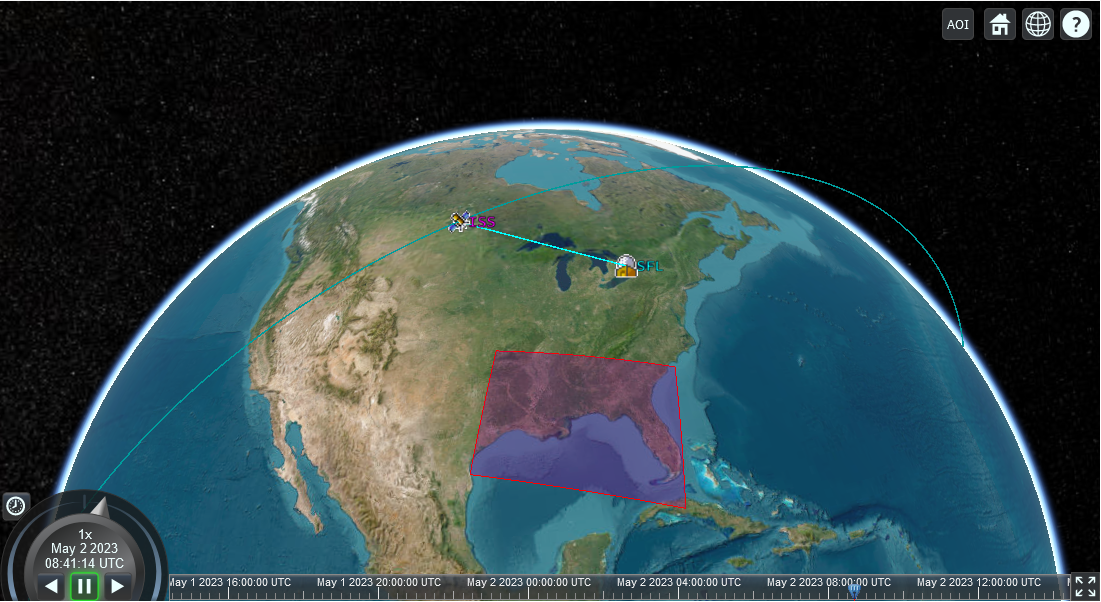
\includegraphics[width=0.9\textwidth]{Cesium_Example_Image.png} 
    \caption{Cesium Example Scenario with Example Entities}
    \label{fig:example_cesium}
\end{figure}

To support this functionality, \gls{pops} makes use of the open-source CesiumJS
library. CesiumJS can display time-dynamic, geospatial information on a
webpage. CesiumJS itself is free to use and provides all of the core
functionality that is necessary for \gls{pops}. There also exists a proprietary
library, CesiumION, which provides out-of-the-box 3D terrain data and
proprietary Earth imagery. Thankfully this kind of information is superflous
for orbit operations planning. At most, all that is needed is a rough
understanding of the Earth's geography and that is sufficient. For this reason,
\gls{pops} does not provide terrain information and uses a free tile map
provider. Since \gls{pops} is only using the free version, we will refer to
CesiumJS as just Cesium for brevity. 

It should be noted that Cesium is only meant to display information to the user
and intended to be a tool that performs any calculations. All data is generated
through other means and then converted into a format that Cesium can display.
The reason for this is that, since Cesium is such a large tool, it is difficult
to validate in great depth because it is not clear what assumptions are being
made at what level. So, as long as the entities being displayed by Cesium are
qualitatively correct then that is sufficient.

An example scenario generated by \gls{pops} can be seen in
Figure~\ref{fig:example_cesium}. There, a few key elements of a Cesium viewer
are visible. On the bottom, there is a timeline with some controls. A user can
change the time of the scenario as they like and the scenario will update
dynamically. This is very similar to tools such as \gls{stk} so an operator
will be used to working in this way. In the centre the Earth can be seen with
the camera hovering over North America.  The camera can be moved with the mouse
or can be fixed to a particular position and orientation programmatically.
Some entities have been added to the scenario. At the bottom, a polygon has
been drawn on the Earth. A very useful feature of Cesium is that polygons can
be defined with vertices and edges clamped to the WGS84 Ellipsoid. That is,
vertices are placed on the Ellipsoid and edges are not straight lines but great
ellipse arcs. This saves a great deal of calculations and code that must be
maintained. Above the polygon, can be seen a satellite, the \gls{iss}, and a
ground station, the \gls{sfl}. The ground station is fixed but the satellite
orbits the Earth and changes position as the time changes in the scenario. The
satellite's path is given by the teal line. 

Every object in the Cesium viewer is treated as a single entity. There are two
ways entities may be added, updated, or removed from a Cesium viewer. Either,
through JavaScript, where a developer creates new objects programmatically, or,
through a custom \gls{json} format called \gls{czml}. Though Cesium has an
extensive client-side \gls{api}, \gls{czml} allows the cesium scenario to be
generated from data rather than from custom code. Most of the underlying data
is calculated through Python scripts so it is more appealing to have an
interface that generates \gls{czml} data rather than having additional
JavaScript. Also, by generating \gls{czml}, logic is not split between the
backend Python code and front-end Javascript. In this way, the Python drives
what is being shown in the Cesium viewer. \gls{czml} also allows for
incrementally streaming data to a client. That is, not all of a scenario needs
to be available immediately once a scenario is loaded. Rather, \gls{czml} data
can be sent in a number of packets, and can be added as they become available.

To set up a viewer, some JavaScript is needed. A placeholder is placed
somewhere in the webpage hosting the viewer then the JavaScript searches for
that placeholder and inserts all of the necessary data to generate the viewer.
Some parameters need to be set for the viewer such as: the imagery provider,
rendering modes, lighting, display options, or toolbar buttons. Once a viewer
is created, it runs until it or the page is changed.  To facilitate
communication between the Cesium viewer and the Python backend, a websocket is
created as they allow for bi-directional communication. 

\subsection{Cesium Models}\label{sec:cesium-models}

Even though we are using Cesium as our 3D Earth visualization tool, a
substantial amound of development must be done to properly configure and manage
what is being shown on the viewer. Before discussing how a Cesium viewer is
managed, it would be useful to first go over what can be displayed currenlty
with \gls{pops}, the Cesium Models. These model classes are not like the ones
made for \gls{orm}, rather these models have two responsibilities. They must
keep some metadata about a Cesium object and they must contain a method that
generates a valid \gls{czml} packet.  A \gls{uml} diagram that summarizes all
of the currently implemented Cesium models can be seen in
Figure~\ref{fig:cesium_models}. It should be noted that the diagram does not
contain an exhaustive list of all of the member variables for each class;
rather, it contains the most important variables.  Each model contains some
information about the object that does not change once it is created. For
example a satellite object will not change which satellite it references once
it's created. 

\begin{figure} 
    \centering
    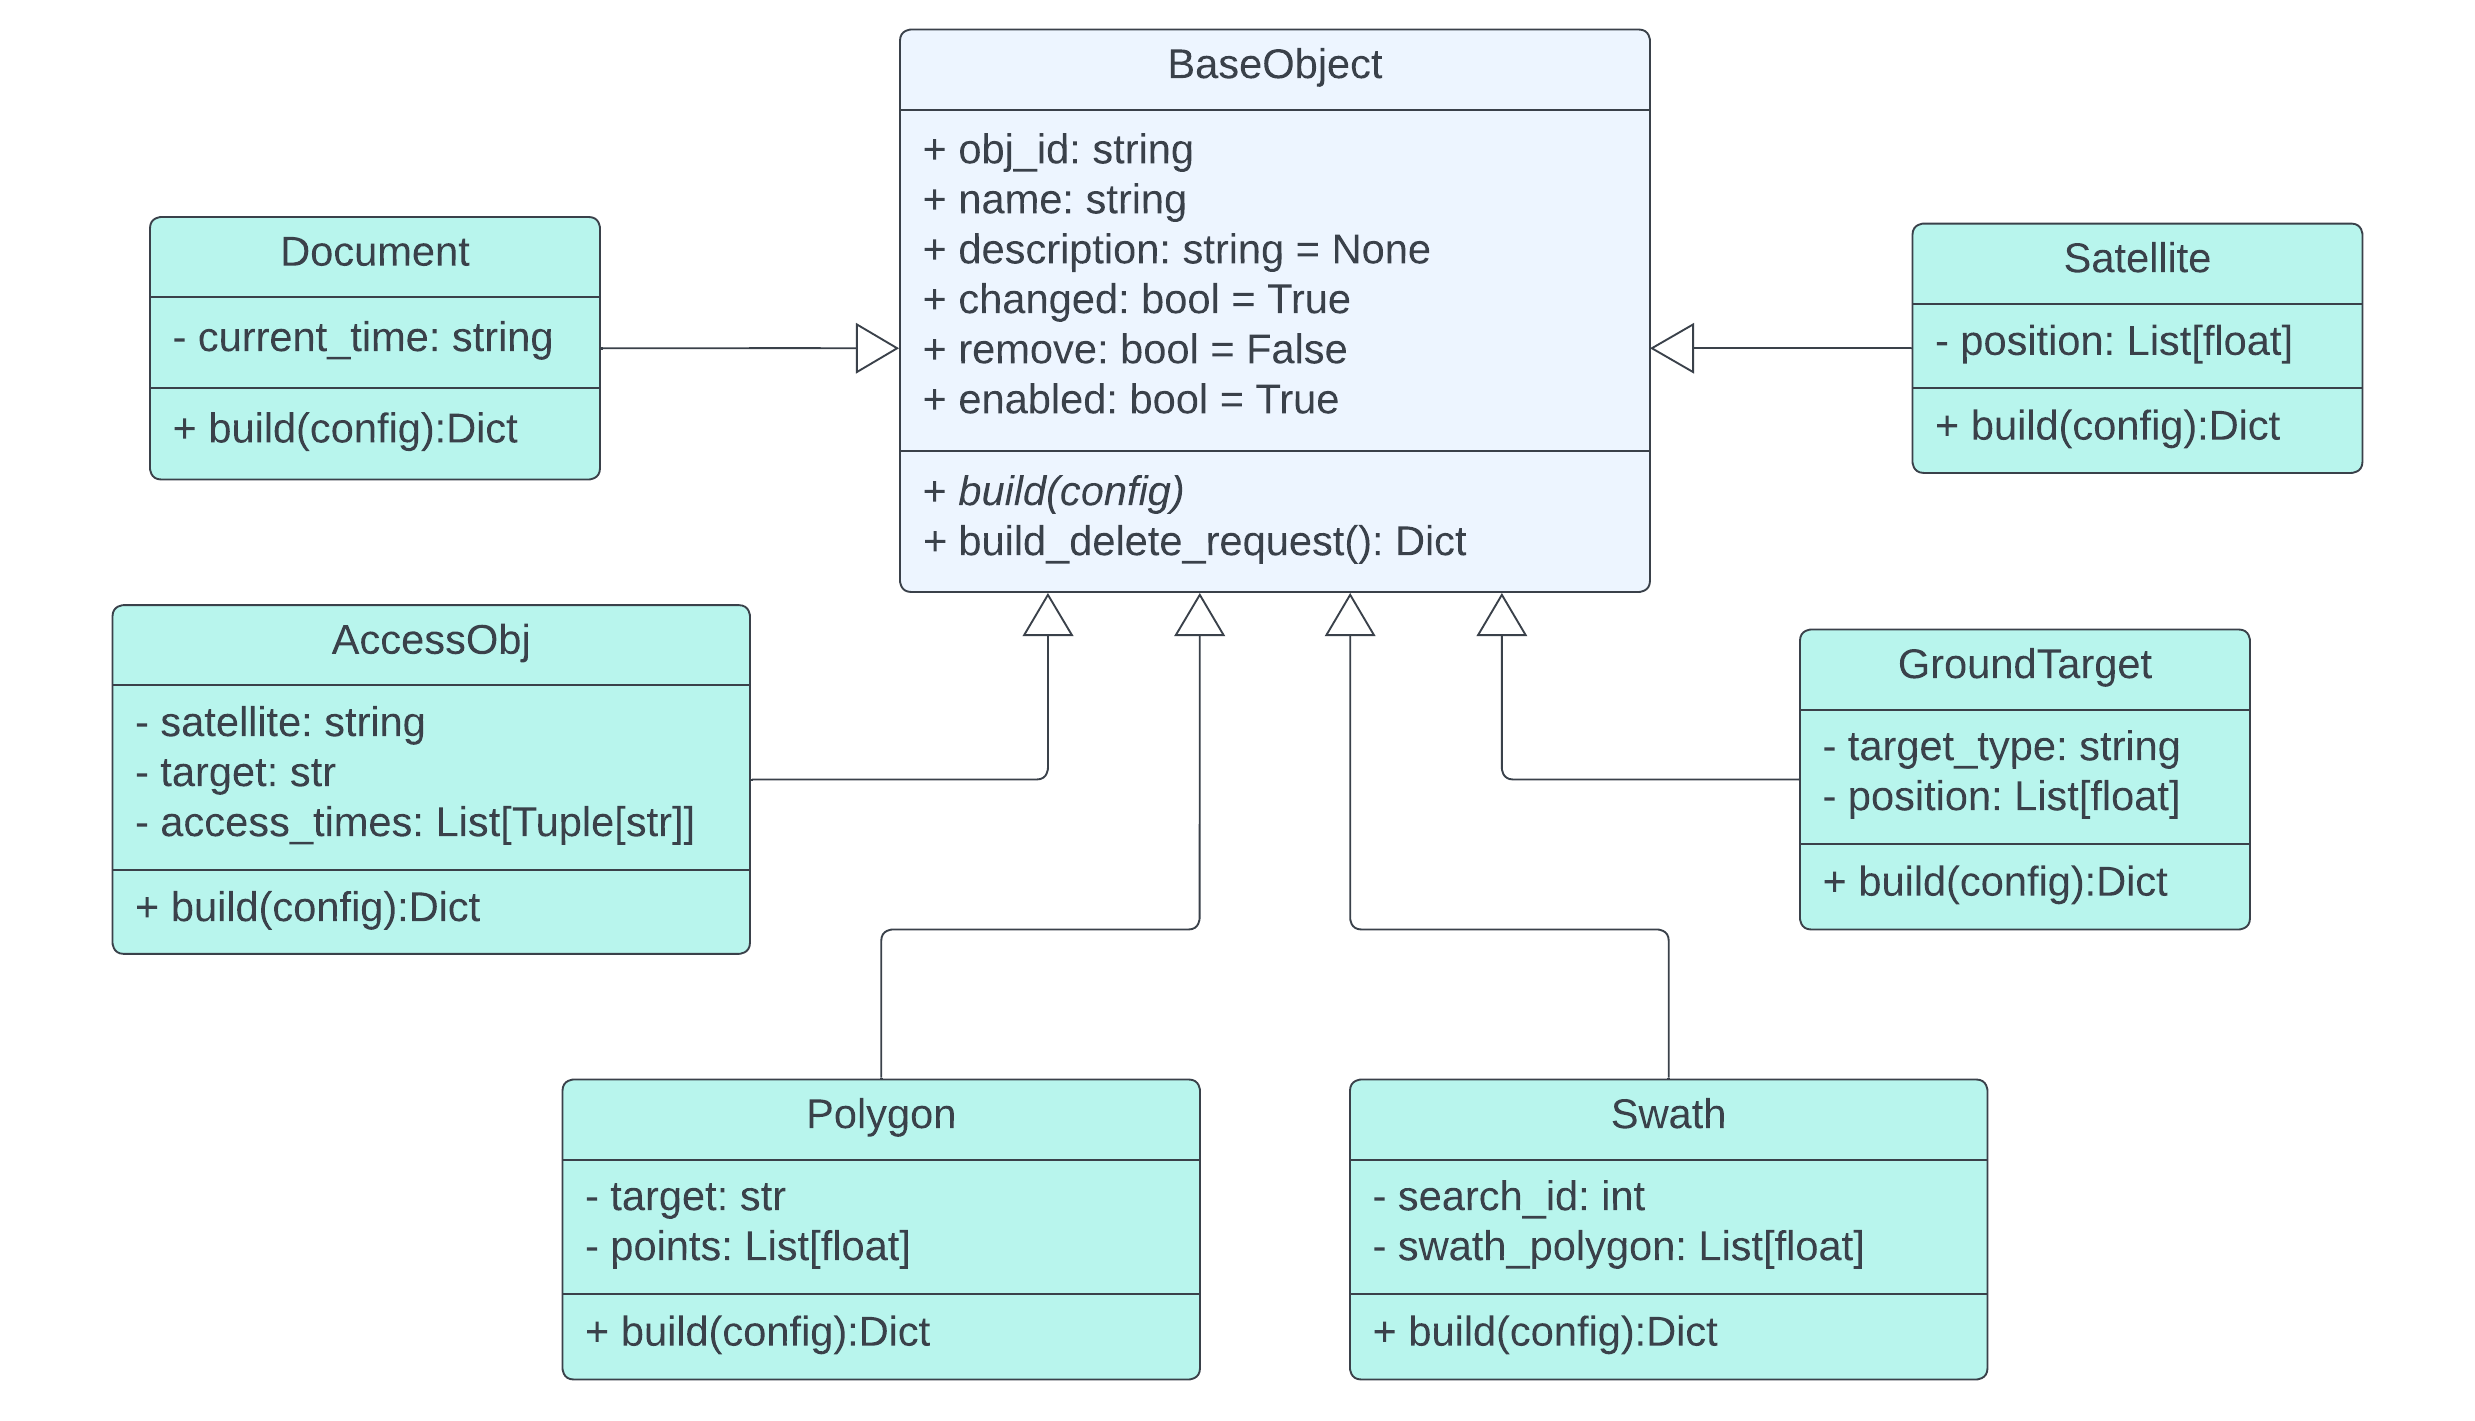
\includegraphics[width=0.9\textwidth]{Cesium_Models.png} 
    \caption{Cesium Models UML} 
    \label{fig:cesium_models} 
\end{figure}

To begin, there is a \texttt{BaseObject} class which serves as a general parent
class to all Cesium objects. It defines member variables that are common to all
objects. Properties such as the object's unique ID, its display name, and its
description. In addition there are three flags that describe the `state' of the
object: \texttt{changed}, \texttt{remove}, and \texttt{enabled}. If the
\texttt{changed} flag is set, this indicates to the Cesium Handler class that a
new \gls{czml} should be generated for that object. By default, every time an
object is created, the \texttt{changed} flag should be set. Once \gls{czml} is
generated and uploaded to the viewer, this flag is reset. If the
\texttt{remove} flag is set, this object should be removed from the Cesium
viewer, and once this is done, the object should be deleted. Lastly,
\texttt{enabled} hides Cesium Entities without unloading them from the viewer.
Each sub-class has its own implementation of the \texttt{build()} method, since
building a \gls{czml} object is unique to that object.
\texttt{build\_delete\_request()} is common to all Cesium objects since the
request only contains the object's ID. The currently supported Cesium models
are as follows:

\begin{description} 

    \item[Document] Each Cesium scenario must have one and only one
	\texttt{Document} object as it specifies general scenario data such as:
	what is the scenario's time range, what is the current time in the
	scenario, or what is the scenario's timestep. Once this object is set
	for a scenario, it does not need to be set again unless the current
	time should be changed.

    \item[Satellite] Satellites are represented through a small \gls{png} image
	called a `billboard'. They are given a descriptive label that maintains
	a fixed position with respect to the satellites position. To have the
	satellite move over time within the scenario, an ephemeris must be
	included in the object. This ephemeris must conform to a particular
	format and this conversion is handled by the Ephemeris data handler
	discussed in Section \ref{sec:data_handler}. Lastly, a satellite is
	given a path to visualize to the user, where the satellite will and has
	been for some period in the future and the past.

    \item[Ground Target] Ground Targets are essentially the same as Satellite
	objects but, in this case, they are given only one position for the
	entirety of the scenario. Ground Targets can be \glspl{aoi}, ground
	stations or any other stationary ground object.

    \item[Access Object] It is useful to display when a satellite has access to
	a ground target. This is accomplished through drawing a polylline
	between the satellite and the ground target for times where they have
	access to each other. One useful feature of \gls{czml} is that we can
	reference the position of other object by reference to their ID. This
	saves us from having to load a satellite ephemeris into the object to
	describe the position of the satellite. \gls{czml} also allows us to
	specify when an object should or should not be visible by specifying
	intervals of visibility. When an \texttt{Access Object} is created we
	must pass a list of access times such that we may define these
	intervals in the object.

\begin{figure}
    \begin{minipage}[c]{0.45\textwidth}
	\centering
	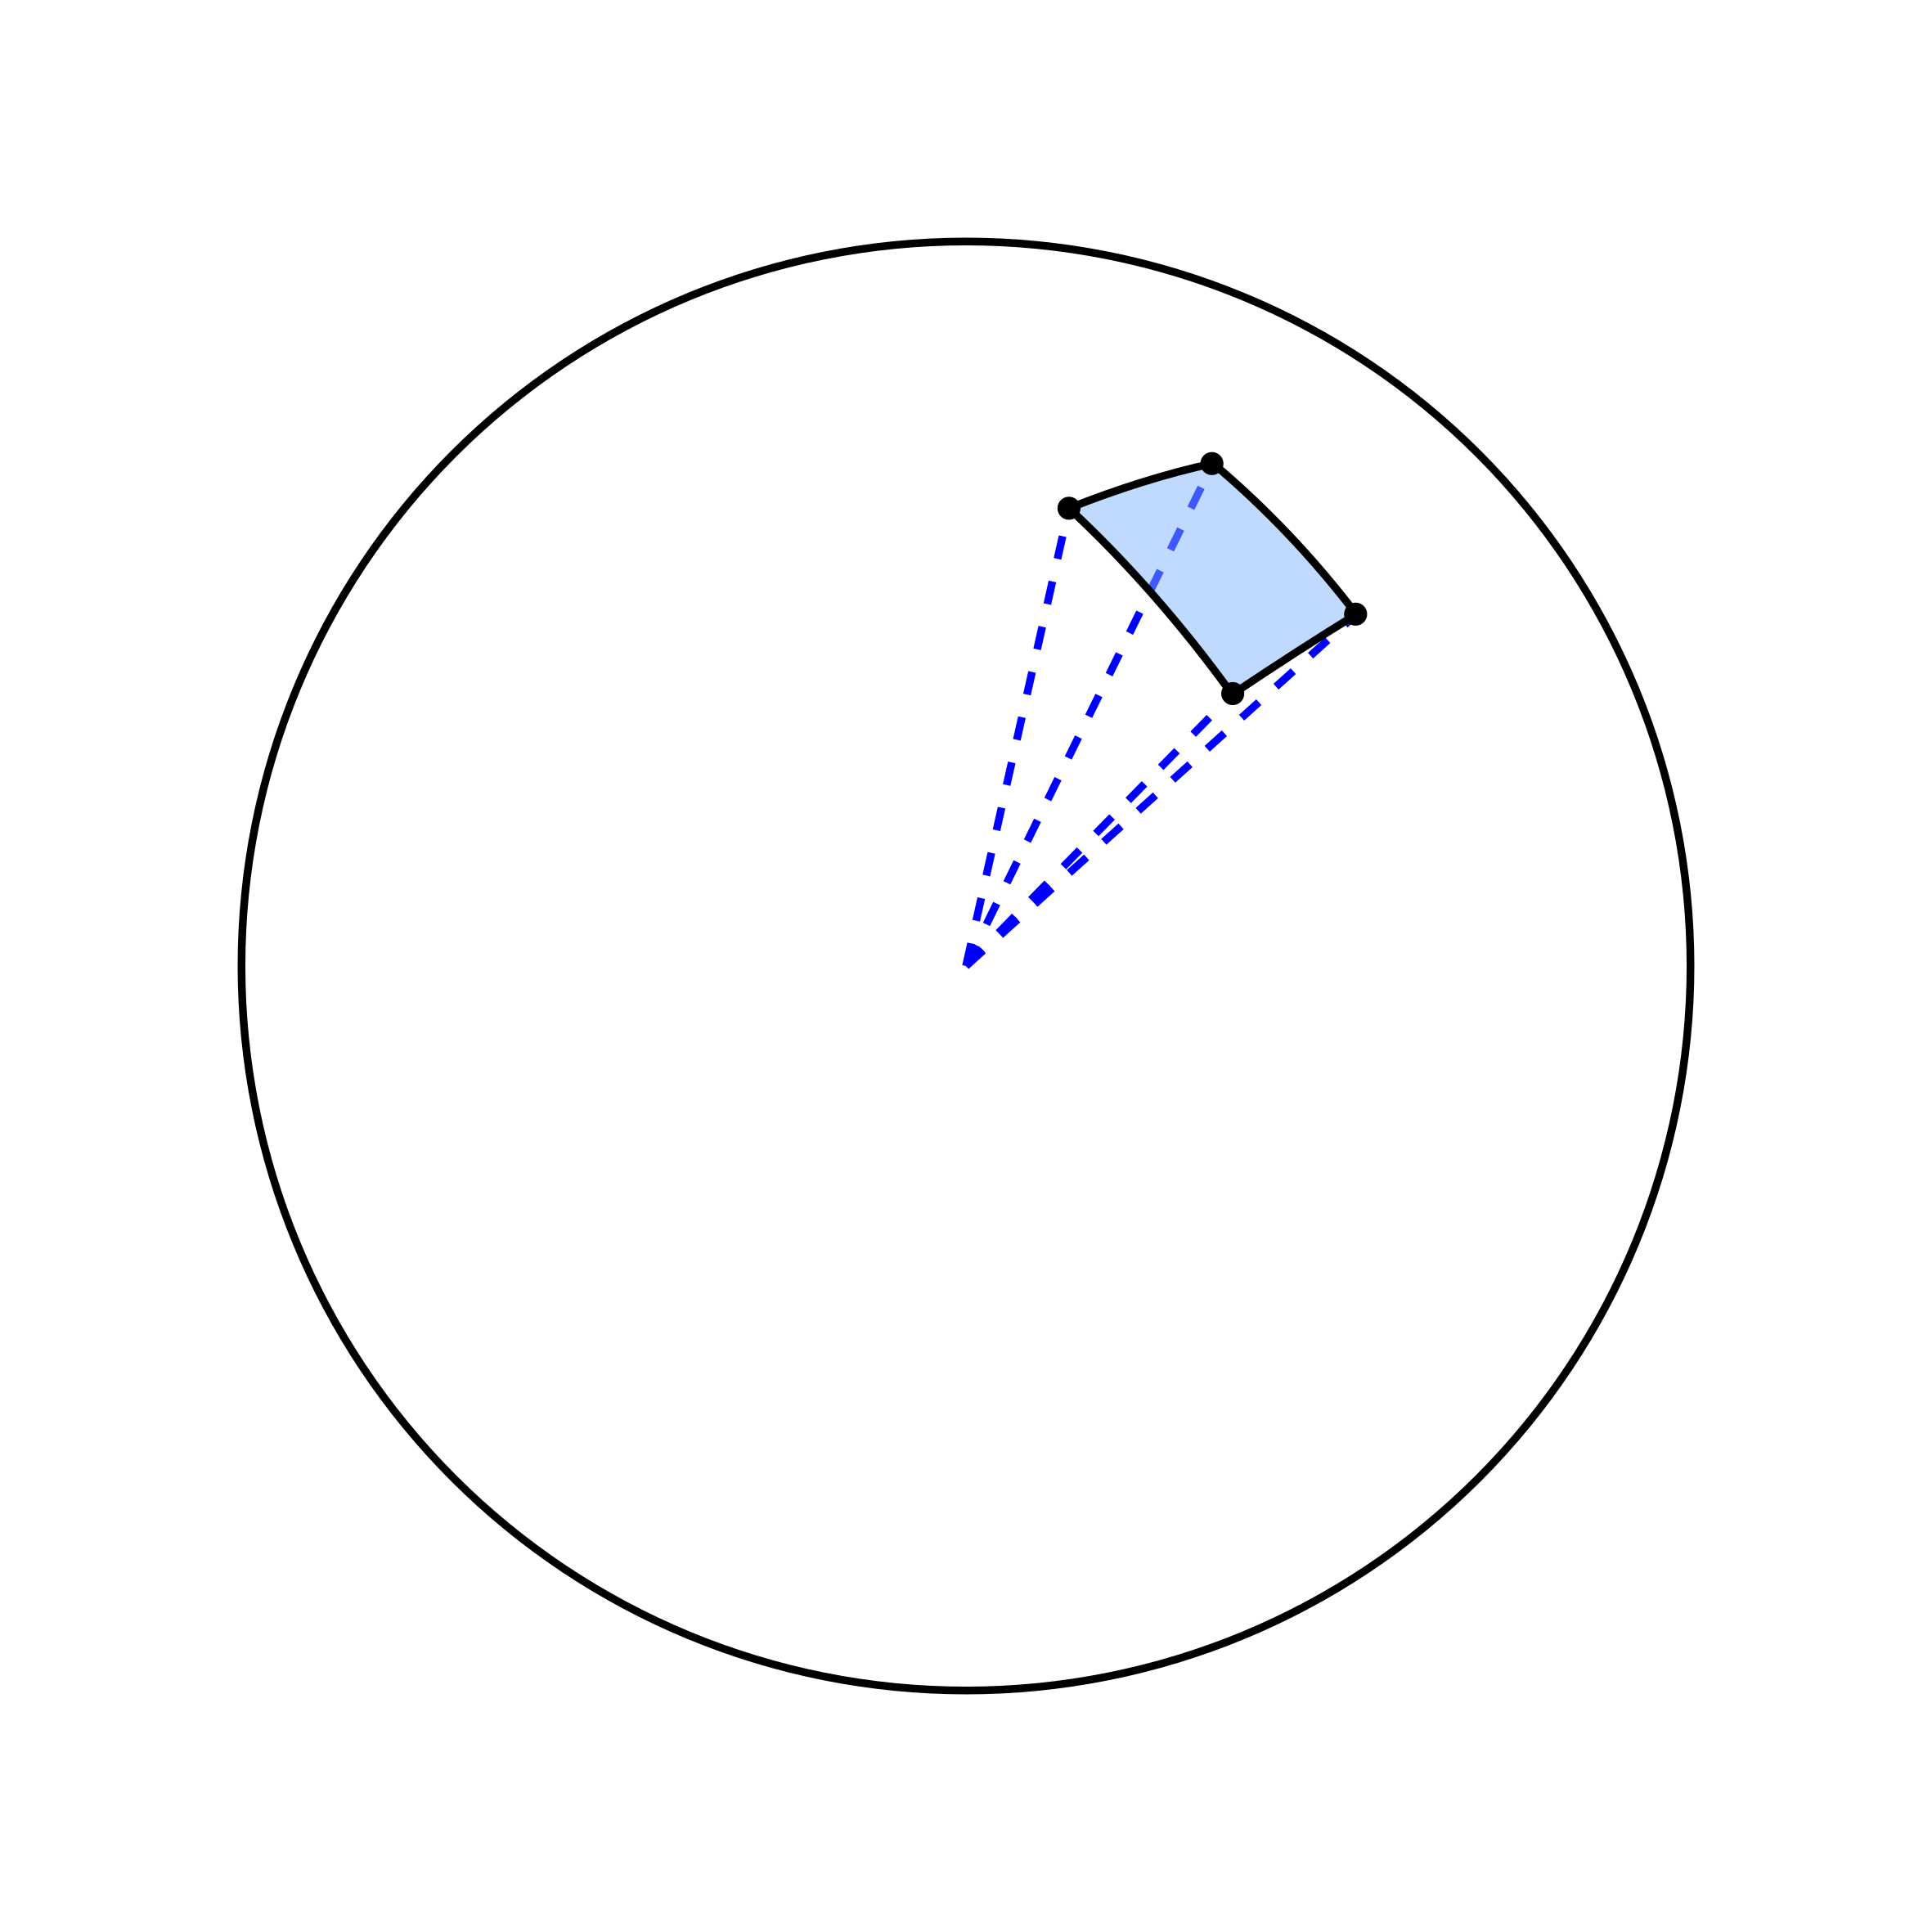
\includegraphics[width=1\textwidth]{inside-outside-2.png} 
	\caption{Smaller Area}
	\label{fig:inside_polygon_1}
    \end{minipage}
    \hfill
    \begin{minipage}[c]{0.45\textwidth}
	\centering
	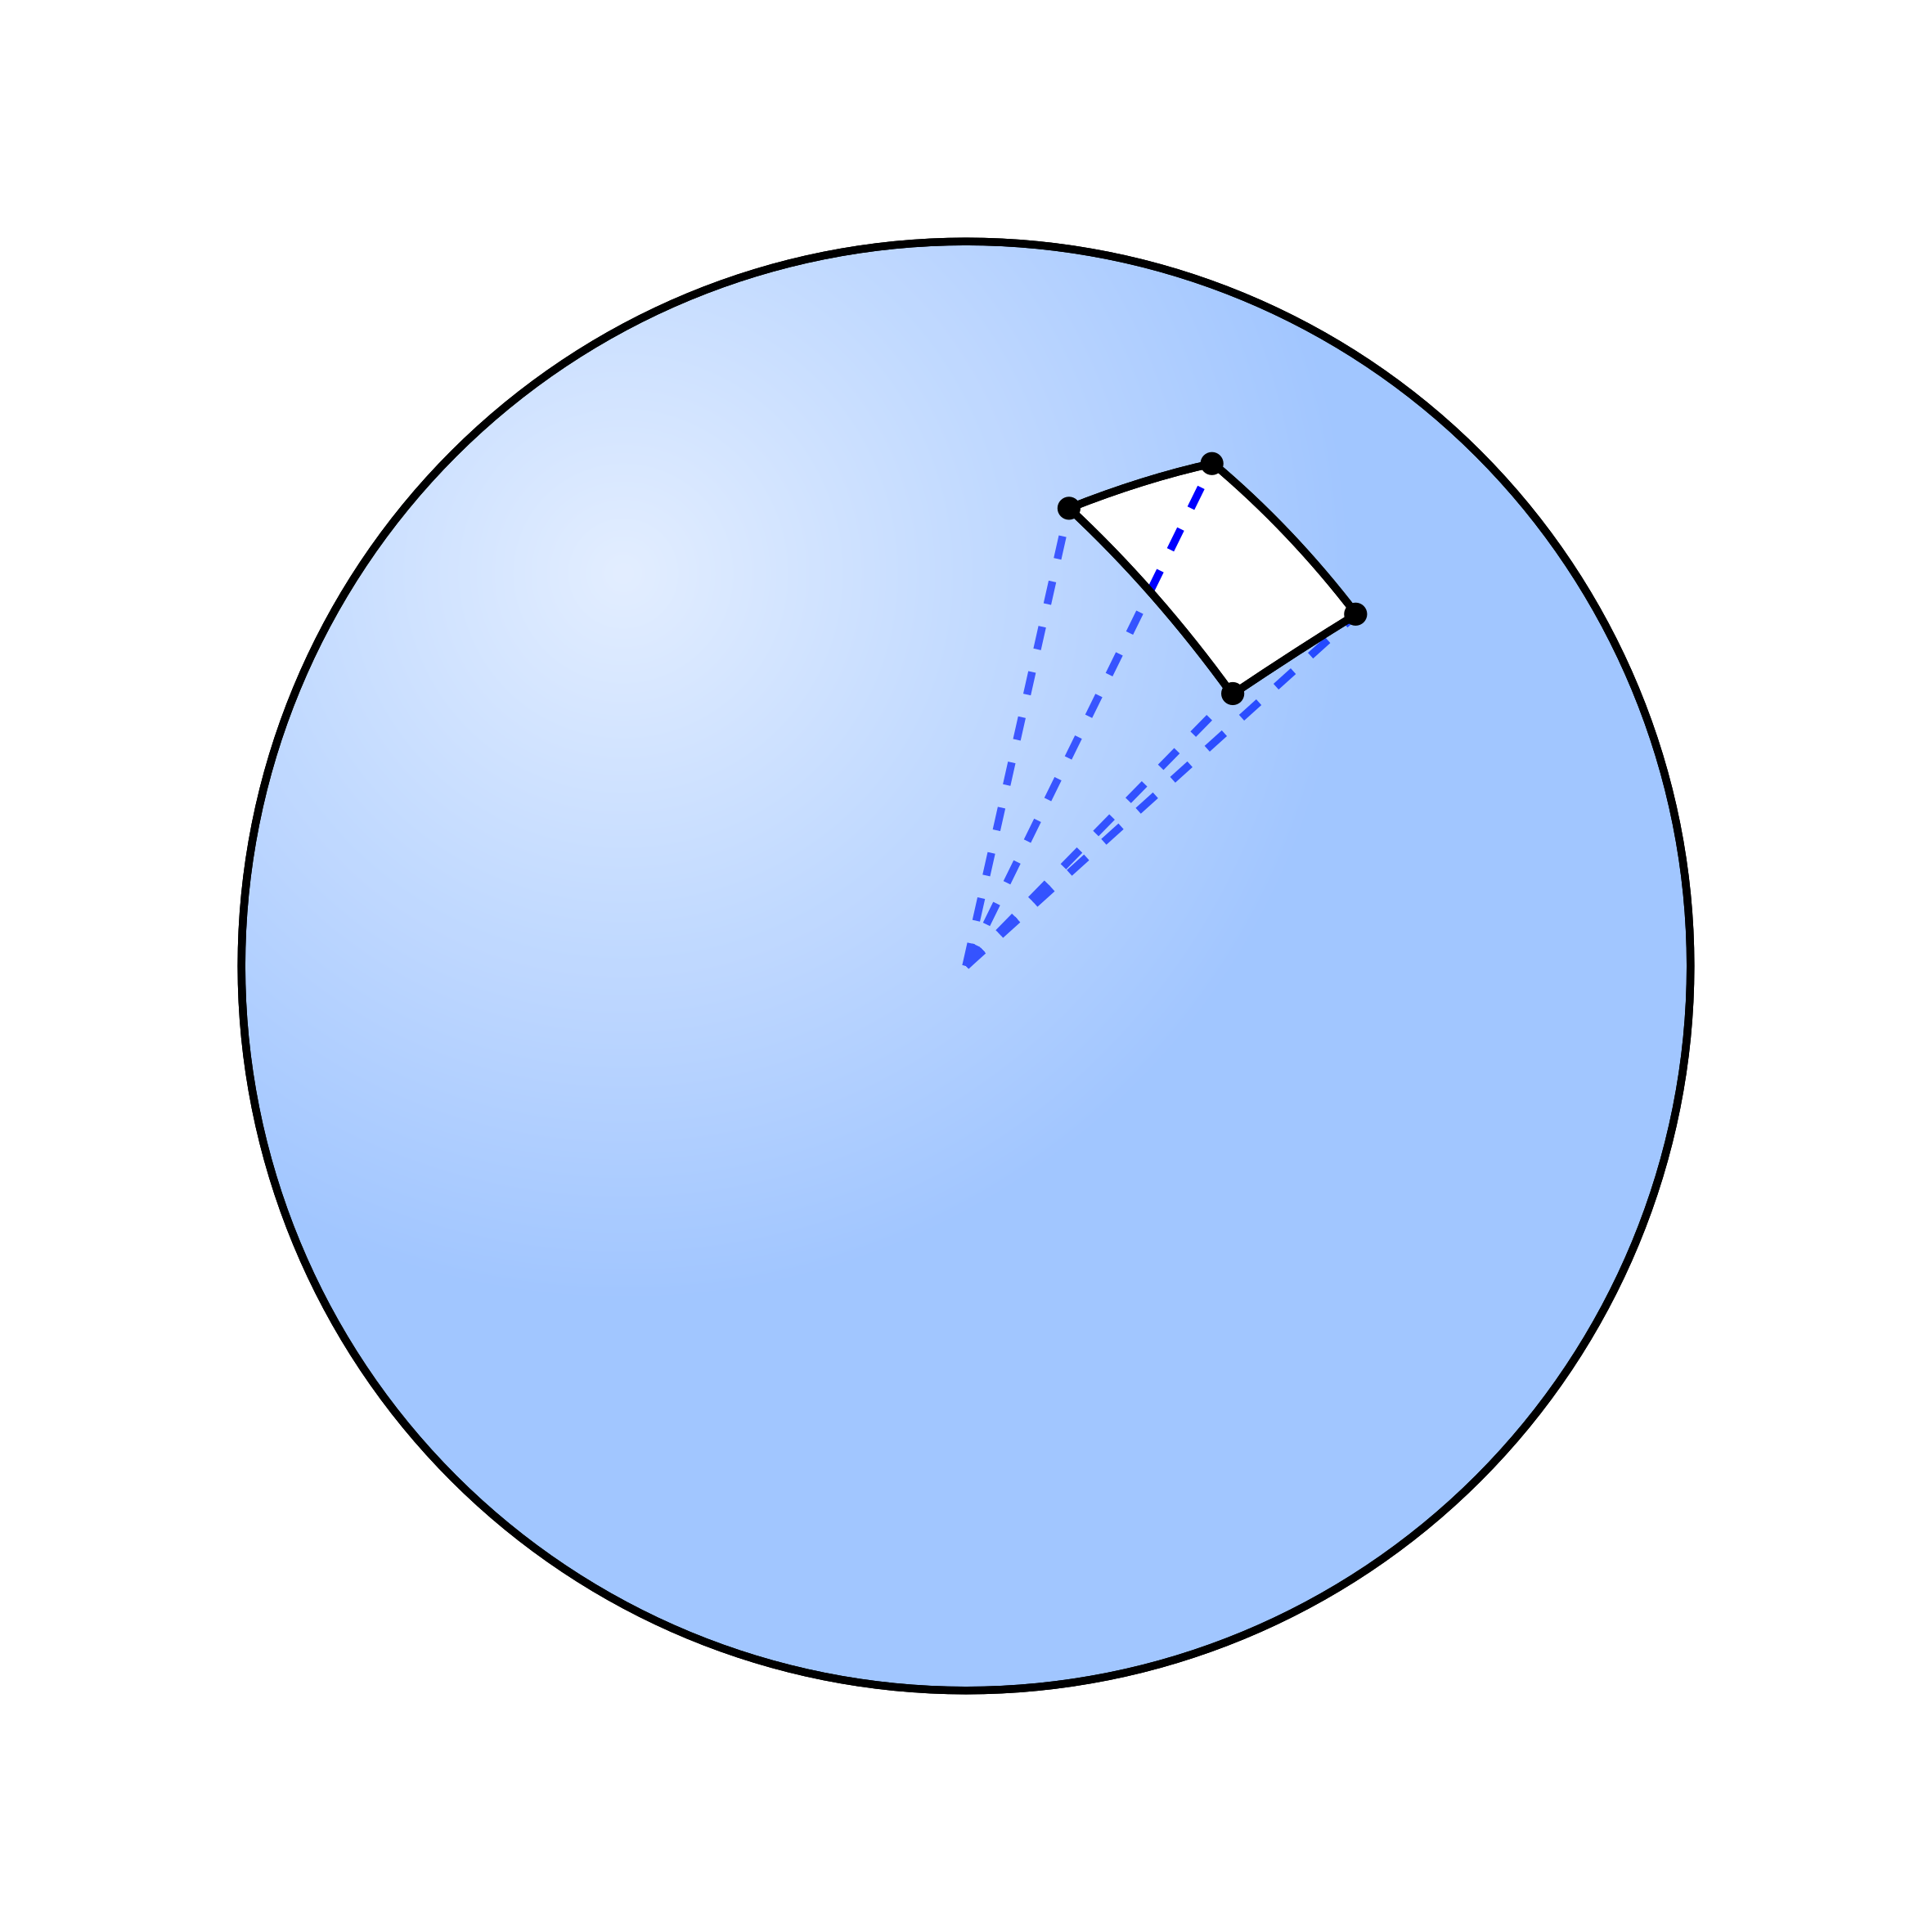
\includegraphics[width=1\textwidth]{inside-outside-1.png} 
	\caption{Wider Area}
	\label{fig:inside_polygon_2}
    \end{minipage} 
\end{figure}


    \item[Polygon] As mentioned earlier, Cesium has the ability to display
	polygons in any number of ways but, for our purposes, we are mainly
	focused on polygons clamped to the Earth's surface. The two instances
	where polygons are currently used for \gls{pops} are for Area Target
	\glspl{aoi} and for intersection polygons. The difference practically
	for these two cases is just in their colour. To draw a polygon in
	Cesium, we must provide it a list of points in Cartesian coordinates or
	in Latitude-Longitude-Altitude coordinates. For the Cartesian
	coordinates, if a point does not directly lie on the WGS84 Ellipsoid,
	Cesium will only draw the closest point on the Ellipsoid. From this
	list of points, Cesium will guess the `inside' of the polygon. Note
	that since we are drawing shapes on an Ellipsoid, the geometry is
	non-Euclidean. The inside of a polygon on a 2D plane is clear for
	polygons that do not self-intersect; it is simply the the region that
	is enclosed by all of the sides of the polygon. For an Ellipse any
	point can be enclosed. See an example of this in Figures
	\ref{fig:inside_polygon_1} and \ref{fig:inside_polygon_2}. Both have
	identical polygons where there are 4 vertices on the Ellipsoid and
	their edges are the same. There is now a question of what forms the
	inside of the polygon as this can be the larger area or the smaller
	area. There are a number of ways this can be addressed. One way is to
	specify the points on the polygon in a clockwise or counter clockwise
	order. Then the internal area will be whatever conforms to this
	ordering. Another way would be to specify one or more points that are
	not vertices but rather example points that lie within the polygon. In
	this way the area of the polygon will be the set of points that contain
	the example point. For simplicity, Cesium makes a best guess at what
	the inside of a polygon is by selecting the inside with the smaller
	area. This is sufficient for smaller polygons but for larger or more
	complicated polygons where the intended area is greater than one half
	hemisphere, determining the inside of a polygon no longer becomes clear
	and the viewer displays a garbled result. Alternatively, if there is a
	polygon which intersects itself, Cesium also becomes confused. In these
	scenarios, a large polygon must be sub-divided into sections that
	Cesium can process.

\begin{figure}
    \centering
    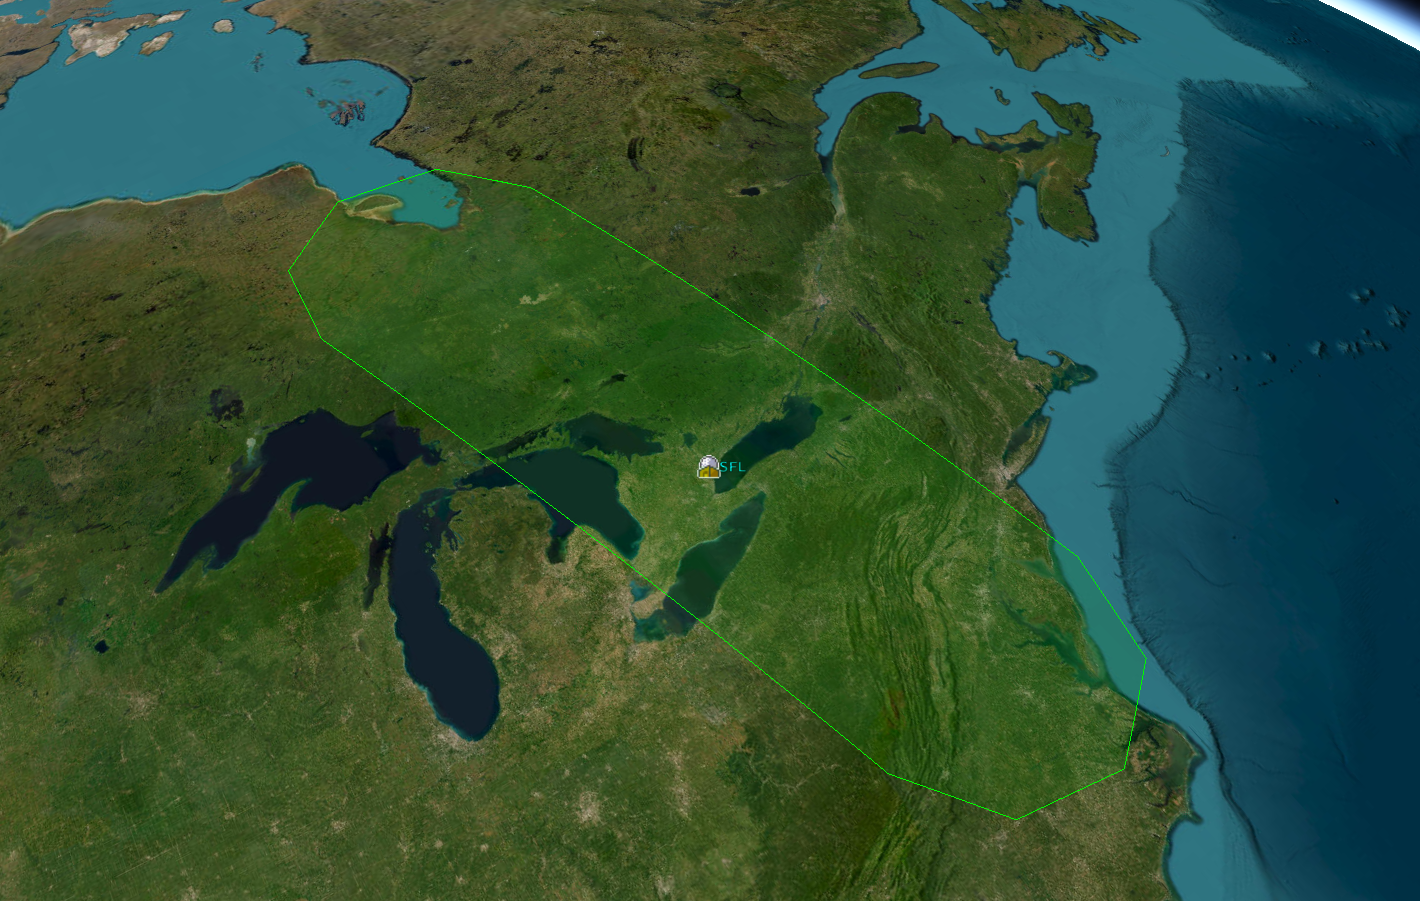
\includegraphics[width=0.9\textwidth]{Cesium_Example_Swath.png} 
    \caption{Example of a 30$^\circ$ Ground Swath}
    \label{fig:cesium_swath}
\end{figure}

    \item[Swath] The last Cesium object that is currently handled are ground or
	access swaths. The distinction here between \gls{fov} and \gls{for} is
	unimportant since both are displayed in the same way. Swaths are
	displayed with polygons but how they are generated can be tricky. From
	the \glspl{atu}, swaths are represented through two polylines that loop
	around the Earth $L_1$ and $L_2$. These represent the left and right
	boundary of the swath with respect to the velocity vector (See
	section~\ref{sec:atu}).  Typically, to display a swath all that we must
	do is reverse $L_1$ and append it to $L_2$. In this way we create a
	counter-clockwise ordered polygon that can be displayed on Cesium. But,
	if we do this for a swath that is defined for greater than one
	half-orbit Cesium will no longer be able to display the polygon because
	it cannot determine what the inside of the polygon is. Thankfully,
	swaths generally only need to displayed for times where a satellite has
	access to an \gls{aoi}. Automatically sub-dividing swaths for longer
	time ranges will be handled in future iterations of \gls{pops}.
	Combining the two swaths boundaries is mostly sufficient for display
	purposes but at the beginning and end of a constrained swath, we may
	wish to show the footprint or access region of the satellite at the
	beginning and end of the constrained swath. To do this, the \glspl{atu}
	also provide ellipse lists for each point in an Ephemeris. From this
	list, we can take the ellipsoids at the beginning and end of the
	constrained swath, take only the points that lie outside of the swath
	area, and append them to the boundary lists. That is,
	\begin{equation*} 
	    P_{swath} = L_1' + E_{start} + L_2 + E_{end}
	\end{equation*} where $P_{swath}$ is the swath polygon, $L_1'$ is $L_1$
	reversed, and $E_{start}/E_{end}$ are the ellipse points at the
	beginning and of the constrained swath. Calculating $E_{start}/E_{end}$
	is somewhat involved and is discussed in Algorithm~\ref{alg:ellipse}.
	An example of a swath can be seen in Figure~\ref{fig:cesium_swath}.

\end{description}


\subsection{Cesium Handler}

Now that we have an understanding for all of the basic objects that are
supported by \gls{pops}, we may now discuss how they are combined to display
mission information to a user. For this, a Python Cesium Handler class has been
written that acts as the interface between the Python backend and the Cesium
viewer frontend. The Cesium Handler class: keeps track of the entities
currently in the Cesium viewer, keeps track of what entities have been changed
or that need to be updated, and generates new \gls{czml} data to be sent to the
viewer. When the \texttt{main} script is first run, it creates an instance of
the Cesium Handler class as a global variable. In this way it can be referenced
as needed by any api call. Some libraries do exist that perform this
functionality but \gls{pops} has enough custom entities that an equivalent
amount of development would need to be done to support them anyway.

To keep track of entities in the viewer, the Cesium Handler class has a list of
objects where each object is a Cesium Model. As such, it has all of the meta
information of the \texttt{BaseObject} as well as a method to build a
\gls{czml} packet and delete packet. By setting up Cesium objects in this way,
they can be treated completely generally by the Cesium Handler class and
metadata can be stored and referenced for every object. This metadata tracks
the status of Cesium objects and determines whether any changes need to be made
in the viewer. 

Objects can be added or removed with helper funcitons in the Cesium Handler
class. Either objects can be added directly, by creating an instance of a
Cesium Model class, then adding them to the list of objects in the Cesium
Handler or a developer can use one of the helper methods. Some situations may
require specific logic to set up a scenario. This is the case for displaying
search scenarios or adding opportunities to a viewer. Currently, there is no
way to generally display the results of a search scenario. A developer must
explicitly define what swaths, intersection polygons, or \glspl{aoi} to add. In
the future this may bemade completely general through some sophisticated but
the current method is sufficient. As with the database, opportunities are also
linked in the Cesium Handler class so that they can be referenced and enabled
or disabled as desired. This makes visualizing search scenarios much more
clear. 

To actual effect changes to the Cesium viewer, the Cesium Handler makes use of
an asynchronous approach. A user may make a change to the Viewer at any time or
they may even make many changes in quick succession and the Viewer must be able
to update correctly. Whenever a change is made to the objects list, first,
\gls{czml} packets are generated for each object whose\texttt{changed} flag is
raised. In this way czml is only sent when necessary and the viewer is not
bombarded duplicate data. These packets are then added to a queue. Then, a flag
is raised in the Cesium Handler class to signal that packets are ready to be
sent to the Cesium Viewer. Within the \texttt{main} script there is a loop that
checks for this flag. Once it is raised, the \texttt{main} service sends every
\gls{czml} packet to the viewer then verifies that the correct number of
packets were received in a return message. If the validation passes, then the
changed flag is reset for all of the objects that were processed. The reason
for using a queue is that it allows for many requests to be processed quickly
without it potentially jumbling the viewer.


\subsection{Scheduler}

The last component of the Mission Model that should be discussed is the
Scheduler Class. The purpose of this class is to keep track of what
observations are planned for all the satellites that are being tracked by
\gls{pops}. The class should be able to: store satellite events, validate
schedules based on some ruleset, and must be able to display all events in a
timeline to the user. 

The base unit for the schedule class are Events. An Event is a general object
that can be used to describe anything. Every Event contains two categories of
data. They have data that is universal to all Events and a payload. The
universal data describes information about the object itself, such as:

\begin{description} 

    \item[ID] The ID of an event which is either a serial number or an
	enumerated descriptive name.

    \item[Name] This is what is actually displayed to the user and may have
	more information than just an ID.

    \item[Type] Is the event a station keeping maneuver, a planned observation,
	a ground contact, etc. The type is arbitrary but it allows events to be
	filtered or treated in different ways.

    \item[Satellite] Each event must be associated with a single satellite. If
	multiple satellites are undergoing an event, each must have their own
	event.

    \item[Time Data] Information such as the start, stop, and epoch of an
	event. An epoch can mostly be ignored but it is important for when
	\glspl{ttc} are created. This is discussed in the \gls{ttc} generation
	section, Section~\ref{sec:ttc-gen}.

    \item[Linked Events] For the case where multiple events are related in some
	way, they may be linked together such that if one is deleted, all other
	linked event may be deleted.

\end{description} 

Along with each event is a Payload. The Payloads allow for specific information
to be stored in an Event without the Scheduler class being aware of what's
there. This functionality will primary be used to contain observation-specific
information such that \glspl{ttc} can be generated from lists of Events without
having the Scheduler class be aware of what observations are possible.
Observations are just one example of how an Events make Events completely
generalizable. In the future, there may be some other type of Event a developer
may wish to store information in. It should be noted that the Scheduler class
will never access or manipulate an Event's payload except to display the
information to a user.

A `schedule' is a universal concept. A satellite has one and only one timeline.
This means that, the scheduler class exists outside off plans or observation
configuration. A plan may add events to a schedule or certain events may be
relevant in a plan but ultimately Events and the timeline exist outside of any
given plan. This is all to say that when a timeline is displayed to a user,
only the parts of the schedule that are relevant to the plan are visible.
Events are filtered by satellites, time ranges, or type. If Events are added to
the schedule by a plan, those events now exist universally for any plan. In
other words, there does not exist one schedule for one plan, it is all the same
schedule.

With this universality in mind, it follows that the Scheduler class has a
1-to-1 relationship with the database. Within the database there is a table of
Events and within the scheduler class there is a list of Events. Every time an
Event is added to the list of Events, a corresponding row is added to the
Database. When the Scheduler class is instantiated, it immediately loads all of
the Events currently stored in the database to its list of Events. The purpose
of this is that \gls{pops} may be shutdown at any time and the list of Events
is retained in the database. By design, there exists no situation where the
Scheduler class differs from the Database.

The Scheduler class also has the ability to validate schedules based on a
library of rulesets. These rulesets are separate add-ons to the Scheduler
class. Within the class, their is a \texttt{validate\_schedule()} method, which
passes the list of events to every ruleset. These rulesets then return lists of
conflicts. These conflicts are stored and displayed to the user graphically and
in a list. The reason why rulests are treated in this way, is that it allows
the Scheduler class to be expandable. Currently, there is only one ruleset and
it checks for time conflicts. For a satellite, do there exist times where 2 or
more Events are scheduled to happen at the same time.  This is a very basic
rule, and it stems from the fact that a satellite cannot be told to do more
than one thing at once. In the future, there will be more rulesets. For
example: the schedule must not exceed a satellite's data budget, the schedule
must conform with a satellite's attitude control constraints, check if Events
are possible with updated weather reports, etc.

Though not currently supported, it is planned that an interface will be
developed that allows events to be generated from ground software. From a list
of \glspl{ttc} that have been uploaded to a satellite, Events will be generated
in the schedule to represent them. In this way, a \gls{pops} user will be able
to see what \glspl{ttc} are already planned for a given satellite. This will
help them develop an operations strategy. This funcitonality will also expand
the usefulness of \gls{pops} beyond just planning.

%% TODO: Add observations to timeline
\begin{figure}
    \centering
    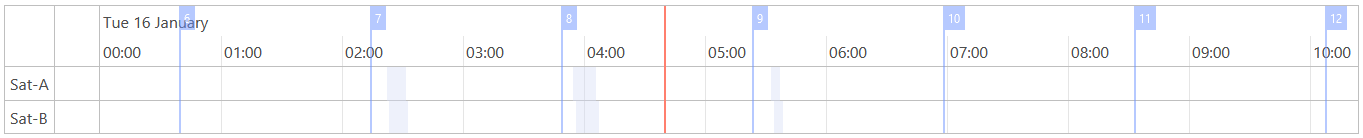
\includegraphics[width=1\textwidth]{timeline-example.png} 
    \caption{\hl{Example of a Timeline}}
    \label{fig:scheduler-timeline}
\end{figure}

The last functionality of the Scheduler class is visualizing a schedule in a
timeline. To do this, the Schedleer class will take a list of Events, filter
them based on the visualization request, format them into a large data packet,
and pass that packet to the webpage. On the webpage, an open-source library is
used to format the timeline. An example of a timeline can be seen in
Figure~\ref{fig:scheduler-timeline}. Observations for each satellite are split
into diffent rows. To give more information to the user, the pass boundaries
are displayed as blue vertical lines. The red vertical line corresponds to the
current time in the Cesium viewer. The shaded regions specify when a satellite
has access to a ground station. Currently, this is all that is displayed is
subject to change based on feedback from operators using the tool.










     
\glsresetall{} 


\chapter{Software Workflow}\label{chap:workflow}

To demonstrate how \gls{pops} may be used, let us walk through setting up
\gls{pops} for the EG-SAT mission. Suppose the customer defines an Area Target
AOI in the Norwegian Sea where they wish Coarse Imaging and Tip-and-Cue Imaging
to be performed. The \gls{aoi} is defined by the points  in
Table~\ref{tab:norway-aoi}. It is the operator’s responsibility to construct an
operations plan for the next week. To do this, they may use \gls{pops} to aid
them in laying out the deterministic aspects of an operations plan.  That
being, determining remote-sensing opportunities, creating a schedule of
observations, validating that schedule, and creating \glspl{ttc} to be uploaded
to the spacecraft. It should be noted that the real-time ground processing of
the data and the generation of new \glspl{ttc} for the next pass of the
Tip-and-Cue Mode are beyond the capabilities of \gls{pops} and this is handled
by separate, mission-specific automatic ground processing.

\begin{table}[h] 
    \centering
    \caption{Area of Interest Definition}
    \begin{tabular}{cccc}
	Point                  & Latitude [$^\circ$] & Longitude [$^\circ$] & Altitude [m] \\ \hline
	\multicolumn{1}{l|}{0} & 73       & -20      & 0        \\
	\multicolumn{1}{l|}{1} & 66       & 19       & 0        \\
	\multicolumn{1}{l|}{2} & 78       & 41       & 0        \\
	\multicolumn{1}{l|}{3} & 82       & 9        & 0        \\
	\multicolumn{1}{l|}{4} & 79       & -17      & 0       
    \end{tabular}
    \label{tab:norway-aoi}
\end{table}

Each step in this process makes use of menus and forms in \gls{pops} that a
user can fill out. To avoid having an excessive number of screenshots for each
step, the input data itself will mostly be shown in tables or figures rather than
through screenshots of the menus.

\subsection{Plan Configuration}

First, \gls{pops} must be configured for a particular mission. The operator
must specify the mission, its satellites, satellite sensor parameters, and its
available ground stations. This will only need to be set once per mission. For
our example scenario, the mission is EG-SAT, the satellites are Sat-A and
Sat-B, and the ground station is the \gls{sfl} in Toronto. The relevant payload
sensors must be specified for each satellite. These are the sensors that affect
payload observations and are referenced by the Opportunity Filter. Currently,
the sensor information is very simple but in the future, this system will be
more developed as \gls{pops}'s modeling capabilities are improved. The sensor
information for Sat-A and Sat-B can be seen in Table~\ref{tab:sensors}. 

\begin{table}[h] 
    \centering
    \caption{Sensor Definitions}
    \begin{tabular}{ccc}
	Satellite                  & Sensor Name & Parameters    \\ \hline
	\multicolumn{1}{l|}{Sat-A} & Coarse      & \{"FOV": 60.0\} \\
	\multicolumn{1}{l|}{Sat-B} & Fine        & \{"FOR": 20.0\}
    \end{tabular}
    \label{tab:sensors}
\end{table}

Relevant ground stations should also be added into \gls{pops}. For each
station the name, location, and elevation mask should be specified. The
location is just in Latitude-Longitude-Altitude. The elevation mask specifies
at what angle, from the horizon, does an object in space become visible; This
is approximated as a single angle. The minimum value for the mask is $0^\circ$,
which is when there are no obstructions at all. For larger mask values, the
less a ground station is able to observe. For EG-SAT, only \gls{sfl} will be
added. Its parameters can be seen in Table~\ref{tab:ground-stations}. It should
be noted that the elevation mask is just an example value.

\begin{table}[h] 
    \centering
    \caption{SFL Ground Station}
    \begin{tabular}{ccccc}
	Station                  & Latitude [$^\circ$] & Longitude [$^\circ$] & Altitude [m] & Elev. Mask [$^\circ$] \\ \hline
	\multicolumn{1}{l|}{SFL} & 43.78   & -79.47   & 193.0  & 10      \\
    \end{tabular}
    \label{tab:ground-stations}
\end{table}

After this is done, the operator will then start creating a plan. Plans lay out
the scenario from which an operator can search for observations and add
them to the schedule. Plan creation begins by specifying the
\glspl{tle} for each satellite.  These can be previous \glspl{tle} stored in
the \gls{pops} database, new \glspl{tle} taken from CelesTrak or Spacer-Track,
or custom-made \glspl{tle} that may be used for simulation or may be more
accurate \glspl{tle} derived from a spacecraft’s onboard \gls{gps} ephemeris.
Once the \glspl{tle} are selected, Ephemerides are generated for each satellite and
stored in the database. For the EG-SAT scenario, \glspl{tle} were generated
with the \gls{stk}. A current limitation of \gls{pops} is that once \glspl{tle}
are selected for a plan, they cannot be changed. Allowing \glspl{tle} to be
changeable would make far too complicated at this stage of development so this
will be addressed in future revisions. For EG-SAT, we will use the \glspl{tle}
in Figure~\ref{fig:tles}.

\begin{figure}[h]
    \begin{verbatim}
    SAT-A
    1 99999U 18099H   24015.66666667  .00000264  00000-0  11261-4 0  0003
    2 99999  96.4575 096.8235 0010629 287.9022 255.6332 15.22959214000011

    SAT-B
    1 99999U 18099H   24015.66666667  .00000265  00000-0  11291-4 0  0007
    2 99999  96.4569 096.8239 0010629 287.8995 250.4360 15.22958218000013
    \end{verbatim}
    \caption{\glspl{tle} For Sat-A and Sat-B}
    \label{fig:tles}
\end{figure}

These \glspl{tle} are artificial and have been created for this scenario. As
such, their NORAD-ID is 9999. Their specifics are not important but, of note,
is that both of their orbits are nearly identical. The only difference being
that the Mean Anomaly of Sat-B is $5^\circ$ less than Sat-A. This means Sat-B
follows the same approximate orbit of Sat-B but it lags behind by some period
of time. Also of note is the reference epoch of both \glspl{tle}, ``2024-01-15
16:00:00.000''.

Once the \glspl{tle} have been selected and confirmed. Ephemerides must be
generated for each satellite in the plan. To do this, the start and end epochs
must be specified, as well as the step size of the propagation. Propagating
\glspl{tle} is generally only accurate $\pm 2$ weeks from the reference epoch
of the \gls{tle}. They may be accurate for more or less time on a case-by-case
basis but, for now, \gls{pops} sets a limit of 2 weeks from the reference epoch
for ephemerides. Any time later or earlier is likely to be inaccurate.
Currently, the step size must be set for the entire scenario. This has become
an issue and will need to be addressed in the future. For long scenarios, such
as 1-2 weeks, having a small step size will yield a large amount of data that
needs to be stored. For a 2 week scenario, at a 10s timestep, one satellite
ephemeris has 120,960 points.  Where each point contains 3 floats for position,
3 floats for velocity, and an epoch string. Some scenarios may have multiple
satellites and this increases the amount of data exponentially. So, for long
scenarios, having a small timestep is not ideal. If a larger timestep is used,
then the opportunity filtering may become less accurate because there is less
information. In the future, more sophisticated methods of ephemeris generation
that better handle data usage will be developed but for now, the step size is
constant for a whole scenario. For EG-SAT, we will create a 3 day scenario
starting at the reference epoch with a 10 second timestep. 

Before continuing, we must also specify what ground stations are relevant to a
plan. Earlier, a ground station was added to \gls{pops} but here we must
associate it with the plan. The reason for doing it in this way is that there
may be scenarios where a mission has a constrained set of potential ground
stations, or other ground stations may become available. Associating ground
stations with a plan allow for them to be configurable. 

Once these settings are confirmed, ephemeris data is generated for each
satellite in the mission and this data is stored in the database. The access
times for each ground station are also calculated for each satellite and that
data is stored as well.


\subsection{Observation Configuration Webpage}

\begin{figure}[h]
    \centering
    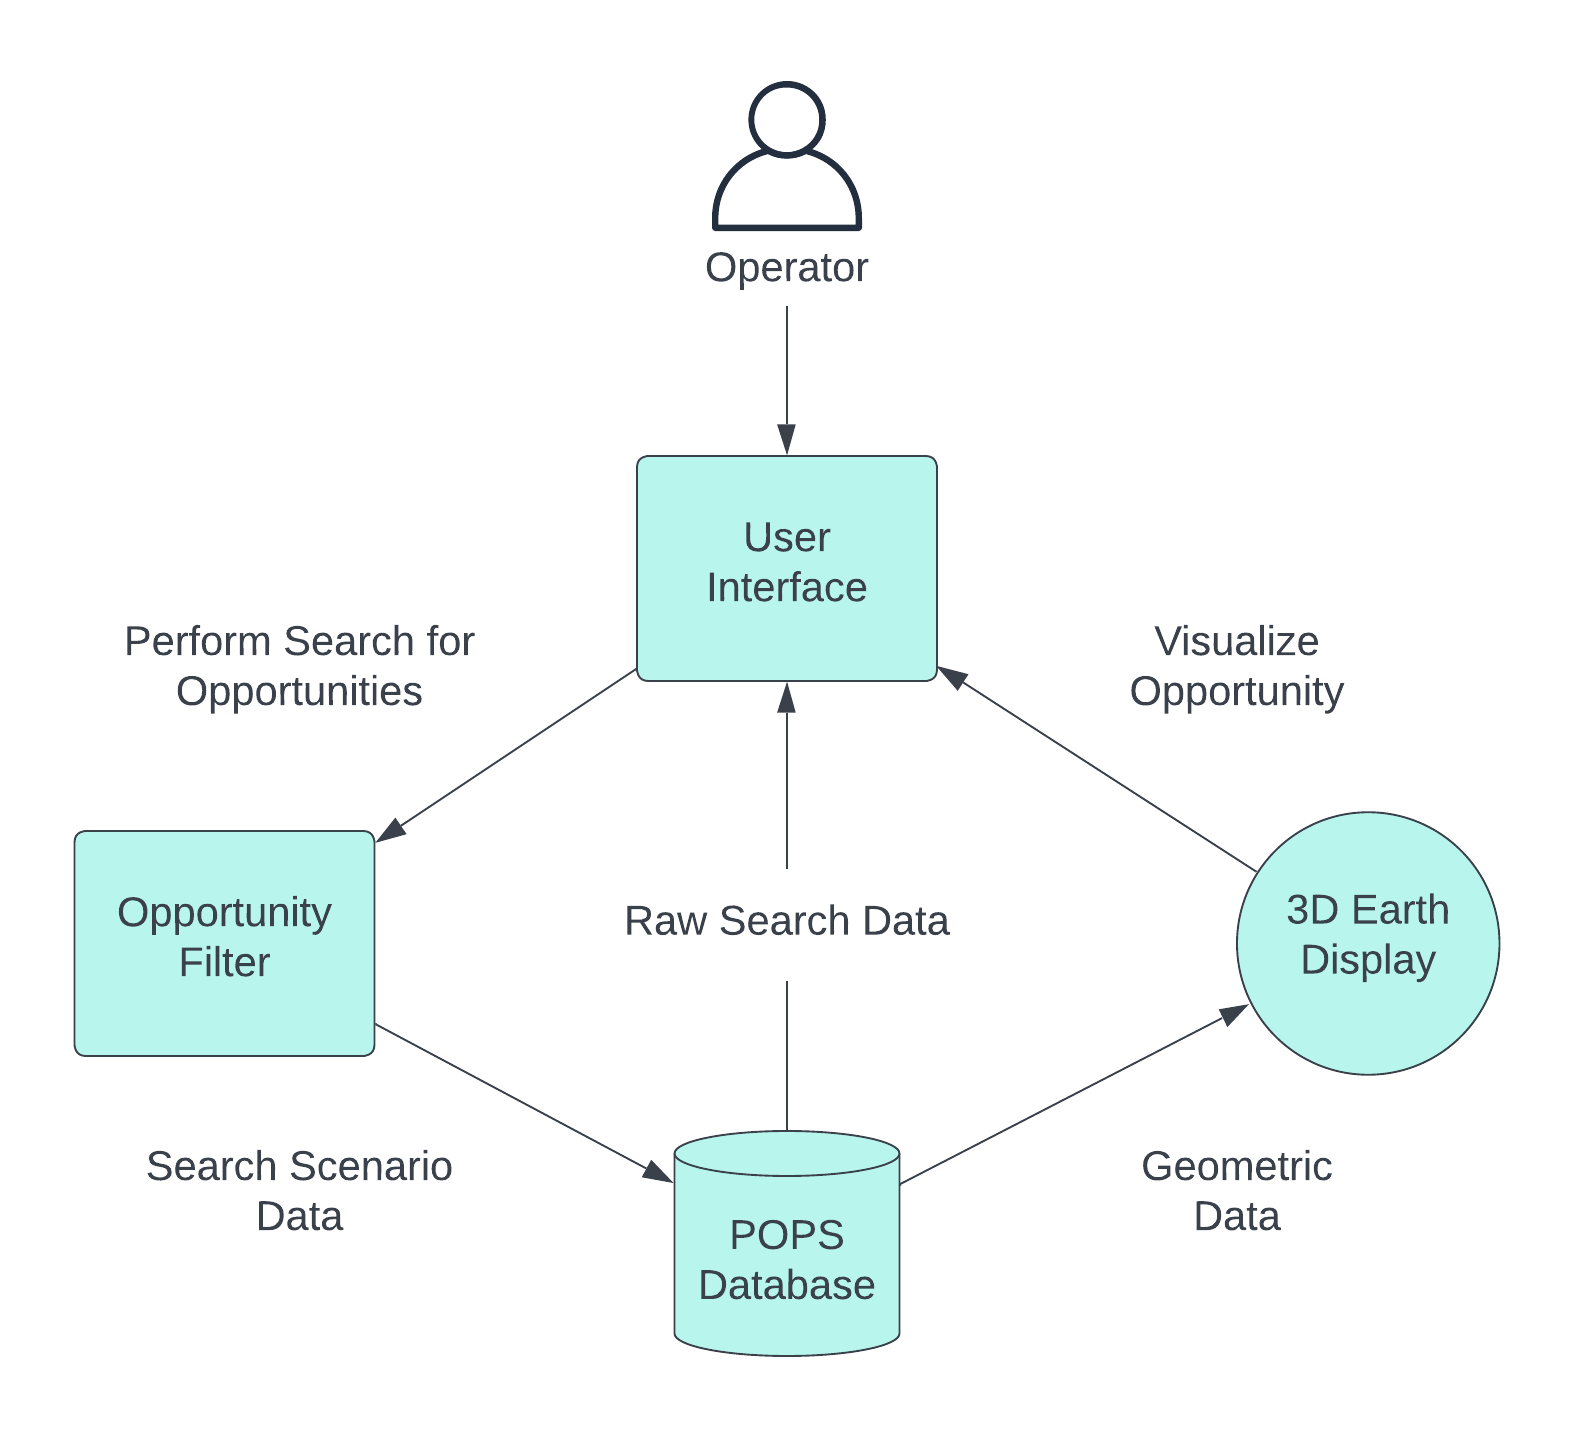
\includegraphics[width=0.5\textwidth]{opp_search_flow.png} 
    \caption{Observation Filtering Summary}
    \label{fig:obs_fil} 
\end{figure}

Once our scenario is set up, we begin Observation Configuration. \gls{pops}
must display potential observation opportunities to the user and must enable
the user to create observations based on these potential opportunities.
Opportunity filtering is the process of taking a large set of potential
observations and constraining them to an \gls{aoi}. Observations can be
performed anywhere on Earth, but we only care about those that provide useful
data for our operations strategy.  The basic process for displaying
opportunities to the user can be seen in Figure~\ref{fig:obs_fil}. An operator
first creates a search scenario through the \gls{gui}.  For a given mission,
there may be multiple observation types, multiple possible \glspl{aoi}, and a
combination of one or more satellites that are part of the observation. All of
this is specified by the user in the form of a search scenario. These
parameters are fed to the Opportunity Filter which generates search data.
Rather than having the search data displayed immediately, all of the generated
search data is stored in the database. From here, it can be retrieved at any
time, without needing to re-compute a search scenario. Some raw search data may
be retrieved and displayed directly to the \gls{gui}. Mostly, these are just
access times.  Alternatively, the raw data may undergo further processing to be
displayed in the 3D Earth visualization. Currently, satellites, satellite
trajectories, ground stations, ground access times, \glspl{aoi}, and swaths can
be displayed.


Since an operator will spend most of their time on the Observation
Configuration page, we shall spend some time discussing it and the utilities
provided with the page. It should be emphasized that \gls{gui}  development is
difficult. A good \gls{gui} and a bad \gls{gui} can functionally do the same
thing but the good \gls{gui} will be easier to use, robust, and visually
pleasing. What's more is that they are extremely time-consuming; hours can be
spent on just a single button, for example. The goal for \gls{pops} is not to
create the perfect user interface but rather the actual functionality itself,
time spent on the webpages themselves is minimized in favor of creating a
functional product. 

\begin{figure}
    \centering
    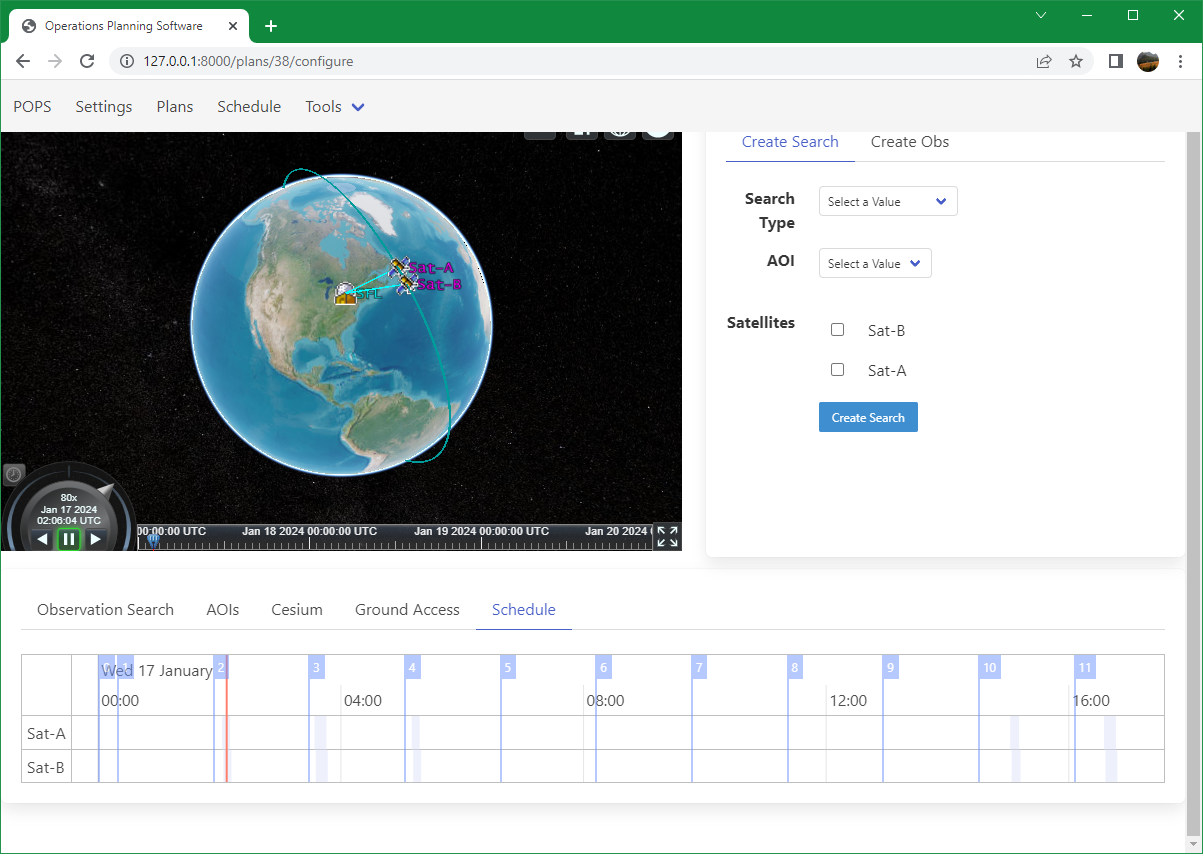
\includegraphics[width=0.8\textwidth]{obs-conf-base.png} 
    \caption{Observation Configuration Webpage}
    \label{fig:obs-conf-base} 
\end{figure}


With that in mind, the Observation Configuration page can be seen in
Figure~\ref{fig:obs-conf-base}. The Cesium viewer is located on the top left of
the page.  There, an operator can see: the Earth, the satellites, their
trajectories, possible ground access times, an Area of Interest, and potential
observation opportunities. In the top right are forms that the user can fill
out to add or make changes to the plan. Currently, that consists of forms to
create search scenarios or to add observations to the plan. The bottom tabs are
meant to display information to the user or allow them to interact with the
Cesium viewer. Currently visible, in the bottom is the schedule timeline.
Here, events are displayed to the user in an intractable viewer. Before going
through how the page is used, the different aspects of the page will be touched
on briefly. 


\begin{figure}[h]
    \centering
    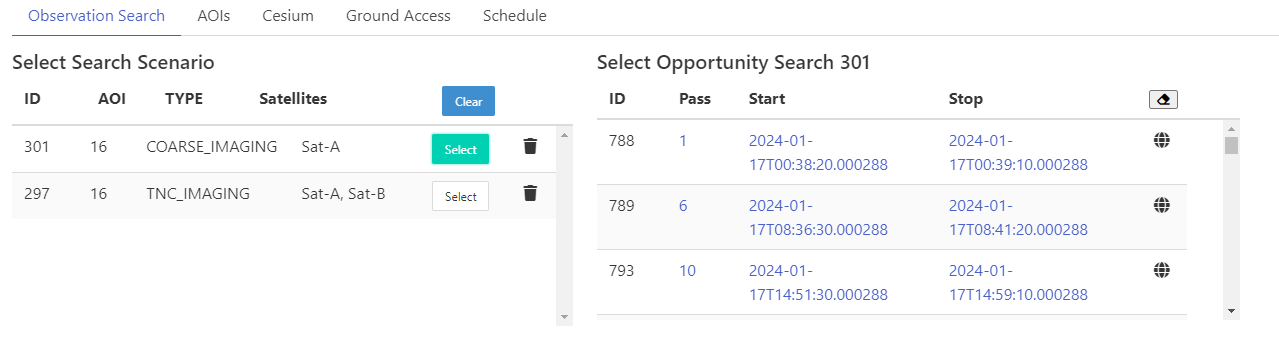
\includegraphics[width=0.8\textwidth]{obs-conf-search.png} 
    \caption{Observation Search Tab}
    \label{fig:obs-conf-search} 
\end{figure}

The results of a search can be seen in the observation search tab in
Figure~\ref{fig:obs-conf-search}. This tab is split into two lists. The left
list displays a list of the search scenarios that are associated with the plan.
When a new search scenario is added, it is added to this list. Here, search
scenarios can be deleted with the trash icon or they may be displayed in the
viewer. For a selected search scenario, the right list displays all of the
opportunities associated with it. Information such as the pass index of the
opportunity, start epoch, and end epochs are displayed to the user. The blue
text entries are hyperlinks. When clicked, they update the current time of the
Cesium viewer. For example, for opportunity \texttt{788} (these are global IDs
not search scenario IDs) if the user clicks on the start epoch, the viewer will
change time to 12:38 AM Jan 17, 2024. The globe icon on the right allows a user
to display or hide an opportunity. Similarly, the eraser icon in the header
toggles the visibility of all opportunities.  The usefulness of these can be
seen in Figure~\ref{fig:obs-conf-ci}.  In Figure~\ref{fig:obs-conf-ci-1},
all of the opportunities in the scenario are displayed. This is of course quite
messy and difficult to understand. In Figure~\ref{fig:obs-conf-ci-2} all of
the opportunities in the scenario have been hidden except for two
opportunities. This makes it far easier to select only the opportunities that
are of interest to an operator.


\begin{figure}[h]
    \centering
    \begin{subfigure}[b]{0.49\textwidth}
	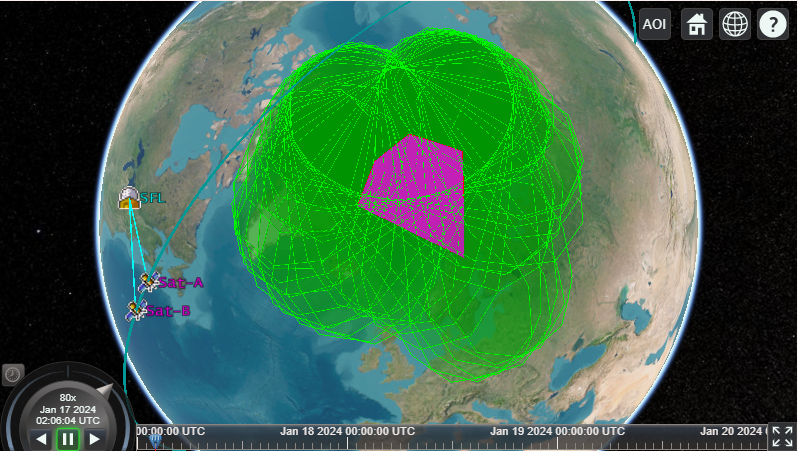
\includegraphics[width=\textwidth]{obs-conf-ces-coarse-1.PNG} 
	\caption{All Opportunities}
	\label{fig:obs-conf-ci-1} 
    \end{subfigure}
    \hfill
    \begin{subfigure}[b]{0.49\textwidth}
	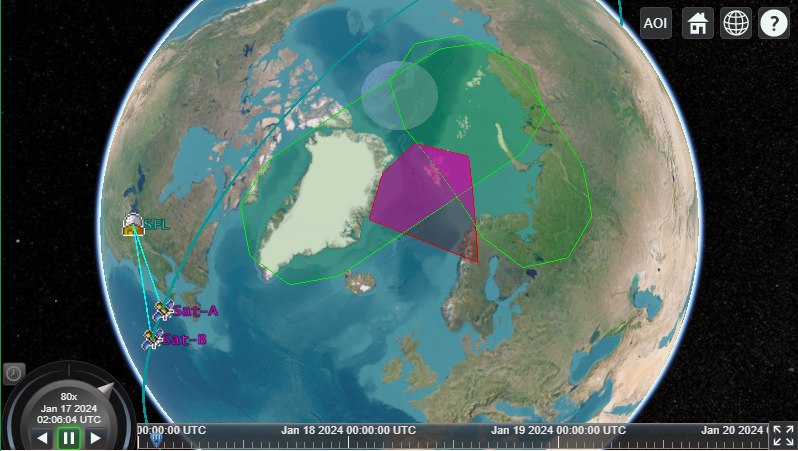
\includegraphics[width=\textwidth]{obs-conf-ces-coarse-2.PNG} 
	\caption{Two Opportunities}
	\label{fig:obs-conf-ci-2} 
    \end{subfigure}
    \caption{Opportunities Displayed in Cesium}
    \label{fig:obs-conf-ci} 
\end{figure}

Every \gls{aoi} that is stored in \gls{pops} can be seen in the \texttt{AOI}
tab. \glspl{aoi} May be added either through a text file that is read and
loaded into \gls{pops}. Alternatively, \glspl{aoi} can be drawn directly in the
Cesium viewer with the \texttt{AOI} button in the Cesium viewer. When it is
clicked, the controls for the viewer change. Every time a user clicks on the
Earth, a polygon vertex is placed at that location. As vertices are added a
white polygon becomes visible. If a mistake is made, the user can undo vertices
by pressing \texttt{CTRL-Z}. To give the user more information, some
instructions are included in a text box as well as the Latitude and Longitude
of the cursor.  Once the user is satisfied, they can right click and the
area-target \gls{aoi} is saved to the database and can be referenced by search
scenarios. A Partially completed \gls{aoi} can be seen in
Figure~\ref{fig:obs-conf-draw}. 

\begin{figure}
    \centering
    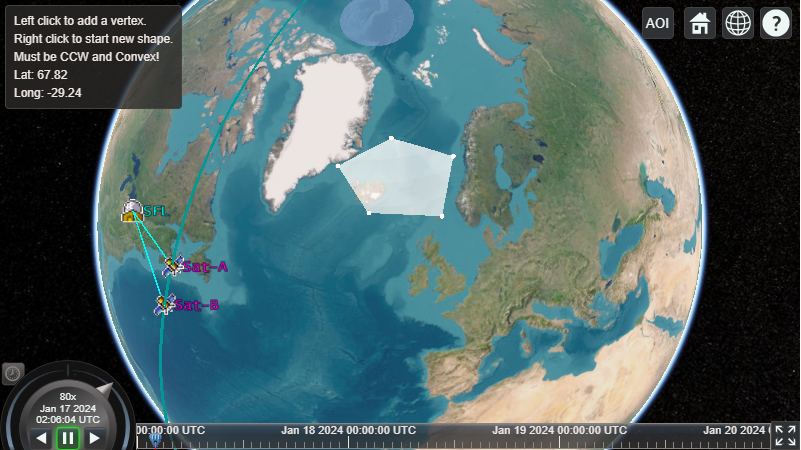
\includegraphics[width=0.8\textwidth]{obs-conf-draw.png} 
    \caption{Drawing an AOI}
    \label{fig:obs-conf-draw} 
\end{figure}

Since there may be many \glspl{aoi} stored in \gls{pops}, a user can display
\glspl{aoi} in the Cesium viewer from the \texttt{AOI} tab. This can be seen in
Figure~\ref{fig:obs-conf-aoi-display}. These `displayed' \glspl{aoi} have red
outlines and purple areas. This is to distinguish them from \glspl{aoi} that
are displayed as part of a search scenario. A useful feature of Cesium is also
viewable in the Figure. When an entity in Cesium is selected, an information
box appears giving the name of the entity as well as its description. Here, the
\gls{aoi} has no description, but from the name, we can tell its: an \gls{aoi},
its ID is \texttt{16}, and it is a display \gls{aoi}.

\begin{figure}[h]
    \centering
    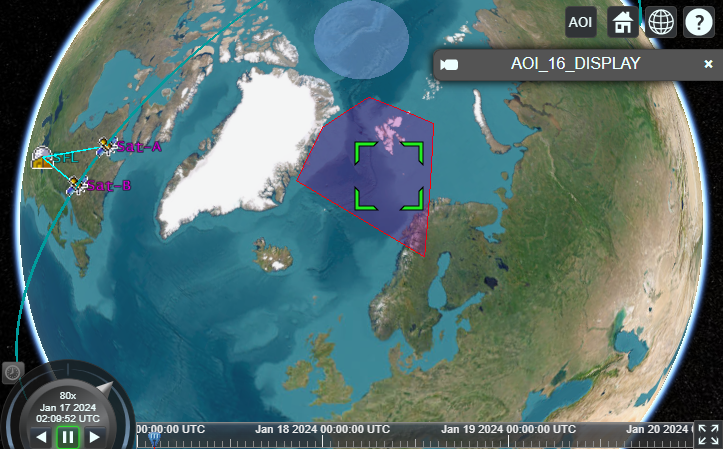
\includegraphics[width=0.8\textwidth]{obs-conf-aoi-disp.png} 
    \caption{Displaying an AOI}
    \label{fig:obs-conf-aoi-display} 
\end{figure}

The last two tabs serve minor purposes. The \texttt{Cesium} tab lists all of
the currently loaded objects in the Cesium Viewer. It allows a user to display
or hide any object. This is mostly useful for debugging, or if a user wants a
specialized view. For example, they may wish to show the intersection polygons
from a number of opportunities. Alternatively, they may wish to compare swaths
from different passes. This tab gives the user the granular ability to make
those changes. The \texttt{Ground Access} tab shows a filter-able list of
ground station accesses, with time links that change Cesium's current time.


\subsection{Searching For Opportunities}

Let us now create two search scenarios, one for the Coarse Imaging Operations
mode and one for the Tip-and-Cue Imaging Mode. To do this we will use the
\texttt{Create Search} tab. In this form, we must specify the search type, the
\gls{aoi} the search should be conducted on, and the  satellites that should be
considered. The search type may be selected from the dropdown. If a user
is unsure about what ID their desired \gls{aoi} is given, they can go to the
\texttt{AOI} tab. There, they may look at the list of \glspl{aoi} and display
them on Cesium for their reference. Earlier in the chapter, an \gls{aoi} was
specified by the imaginary customer in Table~\ref{tab:norway-aoi}. A text file
for this \gls{aoi} definition was written and then uploaded to \gls{pops}. The
ID that was generated was \texttt{16}. This \gls{aoi} can actually be seen
displayed earlier in Figure~\ref{fig:obs-conf-aoi-display}.

\begin{figure}[h]
    \centering
    \begin{subfigure}[b]{0.49\textwidth}
	\centering
	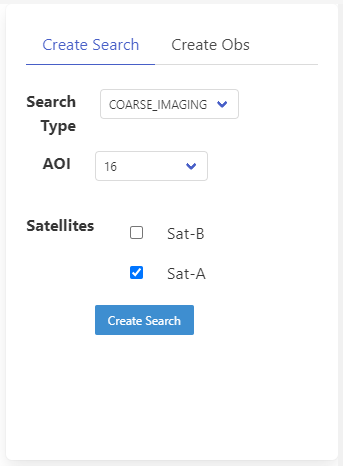
\includegraphics[width=0.60\textwidth]{obs-conf-search-1.PNG} 
	\caption{Coarse Imaging Settings}
	\label{fig:obs-conf-search-1} 
    \end{subfigure}
    \hfill
    \begin{subfigure}[b]{0.49\textwidth}
	\centering
	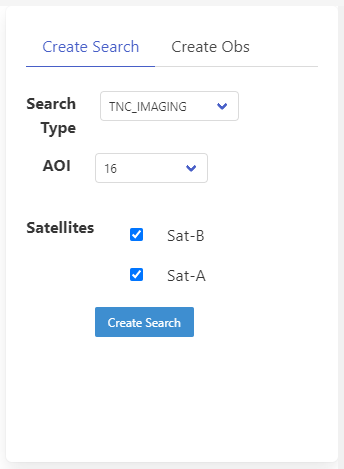
\includegraphics[width=0.60\textwidth]{obs-conf-search-2.PNG} 
	\caption{Tip-and-Cue Imaging Settings}
	\label{fig:obs-conf-search-2} 
    \end{subfigure}
    \caption{Search Scenario Form Parameters}
    \label{fig:obs-conf-searches} 
\end{figure}


For Coarse Imagine the search mode is, of course, \texttt{COARSE\_IMAGING}.
The satellites of relevance for this mode is just Sat-A, because Sat-B is not
equipped with a Coarse Imager. In the future, only relevant satellites will be
selectable but, for now, it is left configurable.  The search form for this
mode can be seen in Figure~\ref{fig:obs-conf-search-1}. Similarly, for
Tip-and-Cue imaging, the mode is \texttt{TNC\_IMAGING} the relevant satellites
are Sat-A and Sat-B.  The mode's settings can be seen in
Figure~\ref{fig:obs-conf-search-2}. Once the \texttt{Create Search} button is
clicked, \gls{pops} will send the data to the Opportunity Filter and a search
will be performed. The two searches can be seen in the \texttt{Observation
Search} tab in Figure~\ref{fig:obs-conf-search}. In the Figure, note that: the
swaths are displayed with green outlines and faint green areas. The \gls{aoi}
has a red outline and a black area, and the intersection polygons have magenta
areas. The Coarse Imaging search mode can be seen in
Figure~\ref{fig:obs-conf-ci}. In total,
there are 43 opportunities for this mode in a 72 hour period. The reason there
are so many is that there are not many constraints for this kind of
observation. All the mode is is a single access time to an area target. 

\begin{figure}[h]
    \centering
    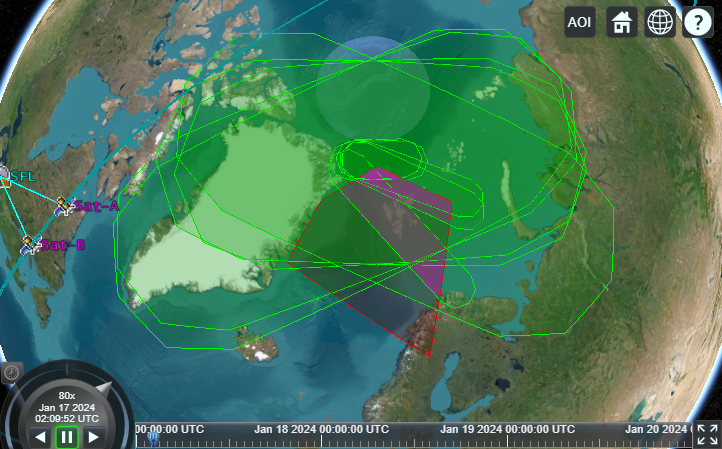
\includegraphics[width=0.7\textwidth]{obs-conf-tnc-all.png} 
    \caption{Tip-and-Cue Imaging All opportunities}
    \label{fig:obs-conf-tnc-all} 
\end{figure}

In contrast, all the opportunities for Tip-and-Cue Imaging mode can be seen in
Figure~\ref{fig:obs-conf-tnc-all}. This view is a bit cluttered but there are
not many opportunities, so individual screenshots have been taken for each
opportunity in Figure~\ref{fig:obs-conf-tnc-opps}. The way each opportunity is
displayed is with two swaths.  The tip swath is the larger one and comes from
Sat-A during the first pass. The cue swath is the thinner swath within the
tip-swath. This comes from Sat-B during the next pass. Note, here the
intersection polygon is the intersection between the tip swath, cue swath, and
\gls{aoi}. For all these opportunities, the tip swath totally encompasses the
cue swath but this is not always the case. In total, there are 5 opportunities
in a 72 hour period. This is far less than there are Course Imaging
opportunities. This is even less than there are general Tip-and-Cue
opportunities. That is, where the cue swath intersects the tip swath and
\gls{aoi}. The reason there are so few opportunities, is because of the ground
station constraint. There must be a ground station contact between the first
pass and next pass. If the satellites are moving from right to left in all of
the views, notice that the tip swaths are all `pointed' at the \gls{sfl} which
is the only ground station. Furthermore, \gls{sfl} is far away from the
\gls{aoi} so opportunities are limited.


\begin{figure}[h]
    \centering
    \begin{subfigure}[b]{0.32\textwidth}
	\centering
	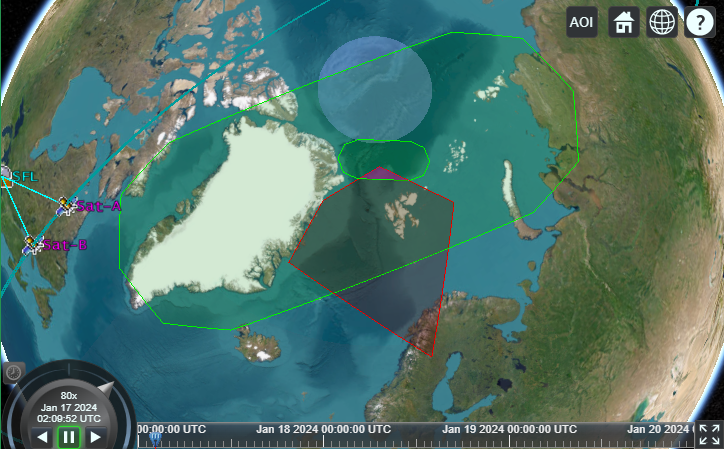
\includegraphics[width=\textwidth]{obs-conf-tnc-1.PNG} 
	\caption{Opportunity 1}
	\label{fig:obs-conf-tnc-1} 
    \end{subfigure}
    \hfill
    \begin{subfigure}[b]{0.32\textwidth}
	\centering
	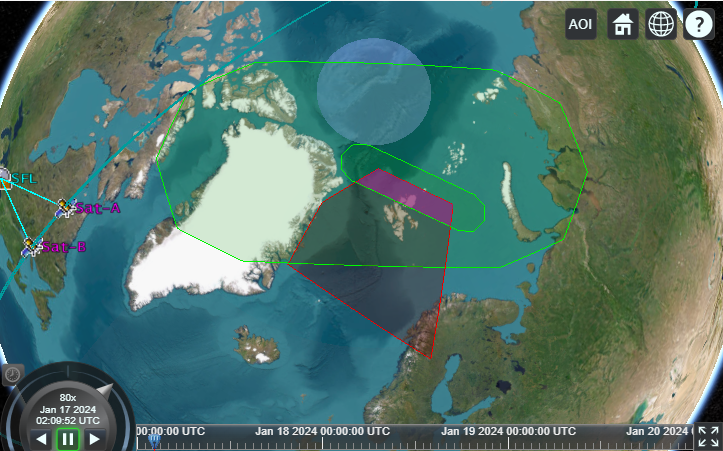
\includegraphics[width=\textwidth]{obs-conf-tnc-2.PNG} 
	\caption{Opportunity 2}
	\label{fig:obs-conf-tnc-2} 
    \end{subfigure}
    \hfill
    \begin{subfigure}[b]{0.32\textwidth}
	\centering
	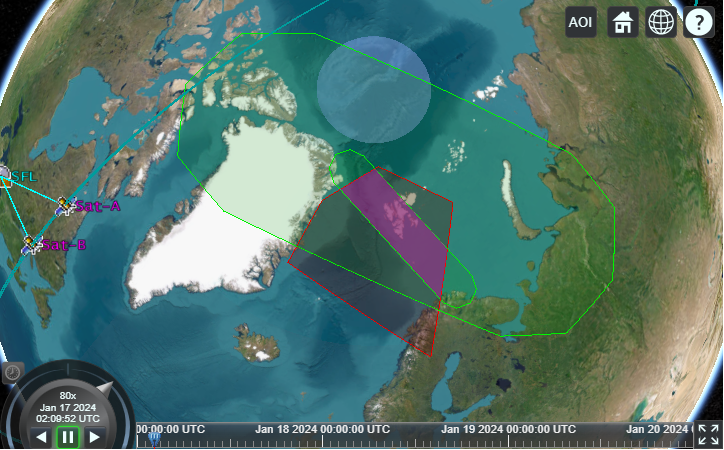
\includegraphics[width=\textwidth]{obs-conf-tnc-3.PNG} 
	\caption{Opportunity 3}
	\label{fig:obs-conf-tnc-3} 
    \end{subfigure}
    
    \begin{subfigure}[b]{0.32\textwidth}
	\centering
	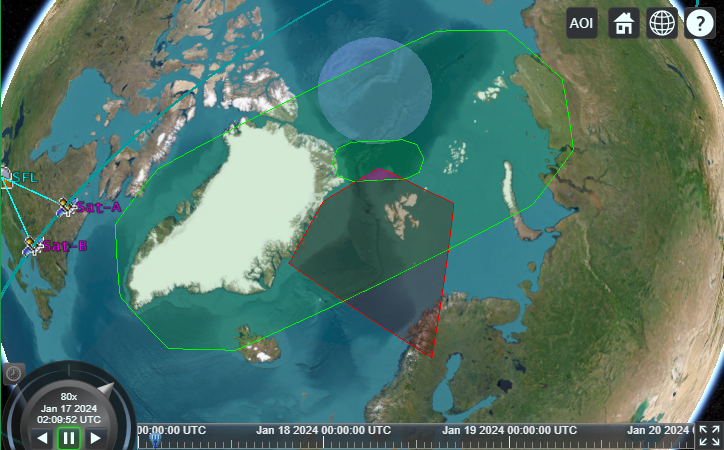
\includegraphics[width=\textwidth]{obs-conf-tnc-4.PNG} 
	\caption{Opportunity 4}
	\label{fig:obs-conf-tnc-4} 
    \end{subfigure}
    \quad \quad
    \begin{subfigure}[b]{0.32\textwidth}
	\centering
	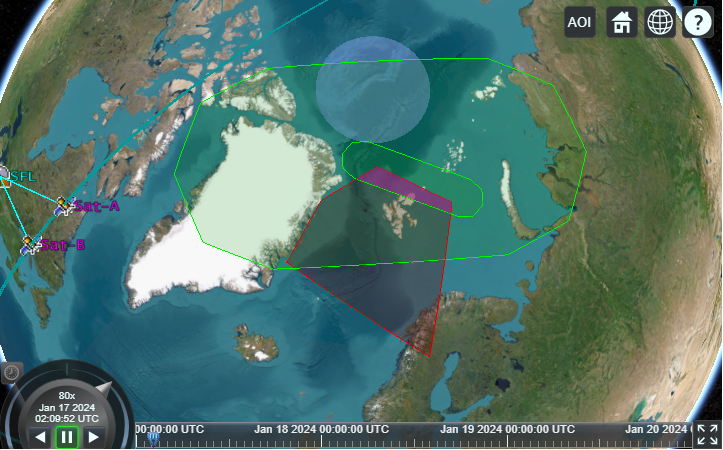
\includegraphics[width=\textwidth]{obs-conf-tnc-5.PNG} 
	\caption{Opportunity 5}
	\label{fig:obs-conf-tnc-5} 
    \end{subfigure}

    \caption{Individual Tip-and-Cue Opportunities}
\label{fig:obs-conf-tnc-opps}
\end{figure}

\begin{table}[h] 
    \centering
    \caption{Plan Summary}
    \begin{tabular}{cc}
	Plan & Stations \\ \hline
	1   &	SFL \\
	2   &	SFL, GSW \\
	3   &	SFL, ESCS 
    \end{tabular}
    \label{tab:additional-plans}
\end{table}

As an example, let us create two more plans with different additional ground
stations, to compare the number of opportunities we can observe. Each plan is
set up identically; the only difference being the ground stations added. If the
plan we have been working with so far is Plan 1, let us create two more plans,
Plan 2 and Plan 3, which have additional ground stations added.  Plan 2 has the
\gls{sfl} and the Weilheim ground station (GSW), near Munich, in Germany. Plan
3 has the \gls{sfl} and the Esrange Space Center Station (ESCS) in Sweden. This
is summarized in Table~\ref{tab:additional-plans}. The parameters for both
these ground stations can be seen in Table~\ref{tab:additional-gs}. The
placements of each ground station with respect to \gls{sfl} and the \gls{aoi}
can be seen in Figure~\ref{fig:obs-conf-gs-placements}. Of course, these are
just example ground stations that have been picked just for this scenario.
Whether they support commercial missions or if they are equipped to support
EG-SAT is not irrelevant. It should be assumed that they can. 

\begin{table}[h] 
    \centering
    \caption{Additional Ground Stations}
    \begin{tabular}{ccccc}
	Station & Latitude [$^\circ$] & Longitude [$^\circ$] & Altitude [m] & Elev. Mask [$^\circ$] \\ \hline
	\multicolumn{1}{l|}{GSW}  & 47.88   & 11.08   & 610.0  & 6      \\
	\multicolumn{1}{l|}{ESCS} & 67.88   & 21.05   & 440.6  & 10      \\
    \end{tabular}
    \label{tab:additional-gs}
\end{table}

\begin{figure}[h]
    \centering
    \begin{subfigure}[b]{0.49\textwidth}
	\centering
	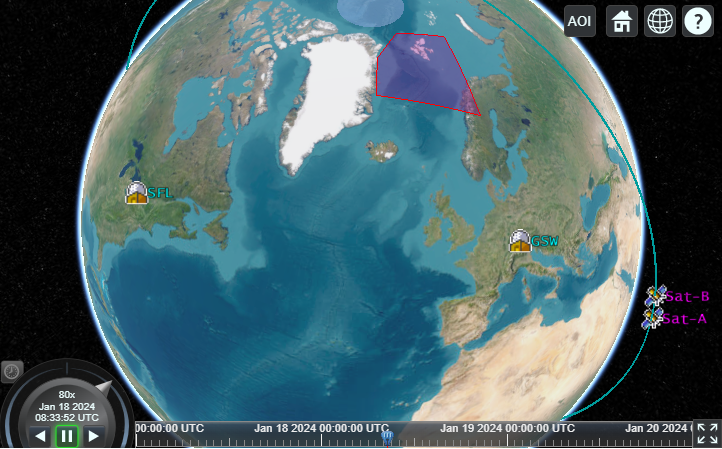
\includegraphics[width=\textwidth]{obs-conf-plan-2.PNG} 
	\caption{Weilheim Station and SFL}
	\label{fig:obs-conf-gs-placements-1} 
    \end{subfigure}
    \hfill
    \begin{subfigure}[b]{0.49\textwidth}
	\centering
	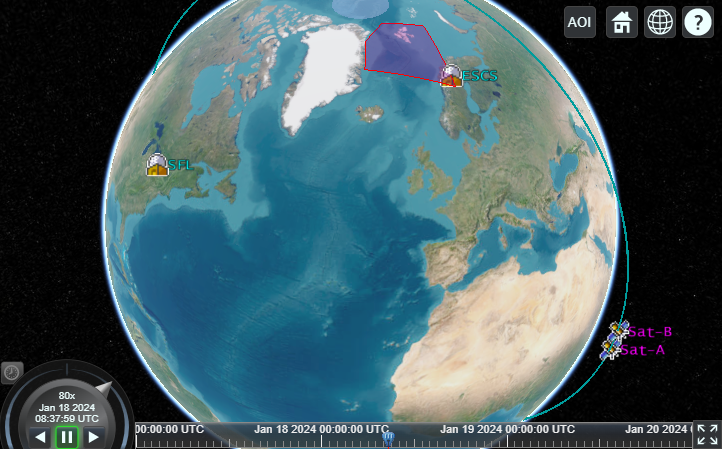
\includegraphics[width=\textwidth]{obs-conf-plan-3.PNG} 
	\caption{Esrange Station and SFL}
	\label{fig:obs-conf-gs-placements-2}
    \end{subfigure}
    \caption{Additional Ground Stations}
    \label{fig:obs-conf-gs-placements} 
\end{figure}

The resulting opportunities can be seen in Figure~\ref{fig:obs-conf-opps}.  For
clarity, the tip swaths have been omitted. As mentioned earlier, Plan-1 only
has 5 opportunities; Plan-2 has 11 opportunities; and Plan-3 has 13
opportunities. It makes sense that with the Weilheim station, more
opportunities will be available since it is located in a different direction
with respect to the \gls{aoi}. Therefore there are accesses for this station
that are not available to \gls{sfl}. The Esrange station happens to be located
very close the \gls{aoi} in this scenario. Therefore, every time the satellites
have access to the \gls{aoi}, it is likely they will also have a ground access
available. 

\begin{figure}[h]
    \centering
    \begin{subfigure}[b]{0.32\textwidth}
	\centering
	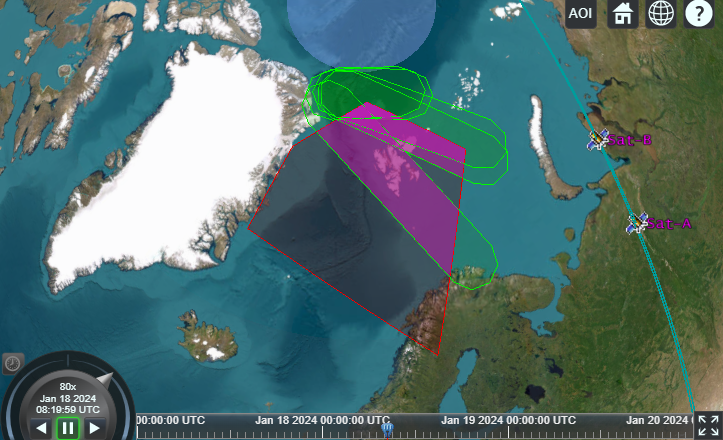
\includegraphics[width=\textwidth]{obs-conf-opps-2.PNG} 
	\caption{Plan 1, 5 Opportunities}
	\label{fig:obs-conf-opps-1}
    \end{subfigure}
    \hfill
    \begin{subfigure}[b]{0.32\textwidth}
	\centering
	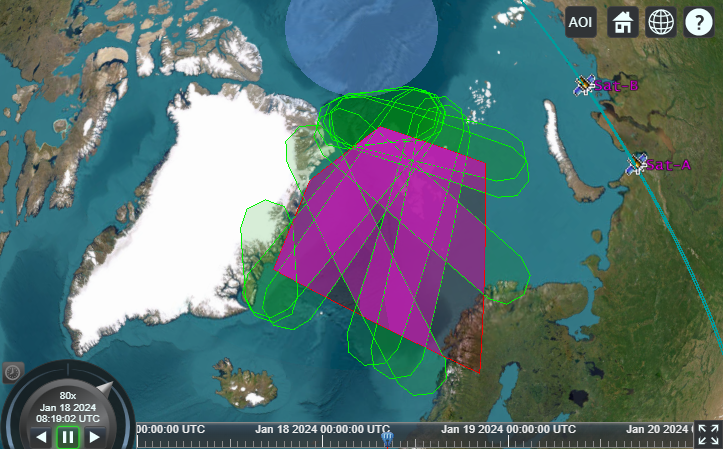
\includegraphics[width=\textwidth]{obs-conf-opps-1.PNG} 
	\caption{Plan 2, 11 Opportunities}
	\label{fig:obs-conf-opps-2} 
    \end{subfigure}
    \hfill
    \begin{subfigure}[b]{0.32\textwidth}
	\centering
	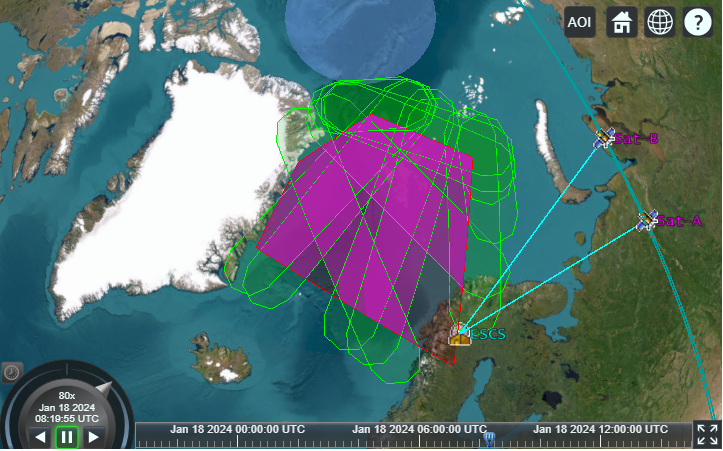
\includegraphics[width=\textwidth]{obs-conf-opps-3.PNG} 
	\caption{Plan 3, 13 Opportunities}
	\label{fig:obs-conf-opps-3} 
    \end{subfigure}

    \caption{Different Plan Opportunities}
    \label{fig:obs-conf-opps}
\end{figure}

For the opportunity filters, there will need to be some fine-tuning going
forward. Edge cases, that were not immediately addressed in their high-level
descriptions or in the actual implementation may have been missed. Questions
like, can one satellite communicate with a ground station while the other is
taking sensor measurements? Are there limitations on ground contacts beyond
just the spacecraft having access? These will be addressed iteratively and the
opportunity filters will be refined through testing and through operations
trials.

\subsection{Creating Observations}

With these opportunities, operators can then create observations. Currently,
this is a manual entry process. An operator must specify both the epoch of an
observation as well as the duration. For the Course Imaging mode, this will
just be a single event. For the Tip-and-Cue mode, this will be both a tip event
and a cue event. In the future, these observations will be added straight from
the list of opportunities. Nominally, an opportunity should correspond 1-to-1
with an observation. There may exist some parameters that need to be set for
the purposes of \gls{ttc} generation, so a form is still necessary and the
process cannot be completely automated. This system is being reworked and
hasn't been fully integrated at the time of this thesis being written.


\subsection{Scheduling}


Once observations are added to a plan, they must be added to the schedule and
validated. The schedule is universal to any observation, plan, or mission and
is used to describe what actions a satellite may perform. Events may be added
through the observation configuration page or an interface with \gls{sfl}’s
other ground support software. The interfaces have not yet been developed and
will be future additions to the software.

Finally, once events are added to the schedule, the schedule is then validated.
Validation is based off of a library of validation rules. All events are
evaluated with each rule and any conflicts are logged. Currently, only one rule
has been implemented; that being: no two events may happen simultaneously on
the same satellite. More rules will be added such as: observation specific
rules (a plan must conform with a satellite’s data budget), attitude control
considerations, as well as the weather forecast. Again, \gls{pops} is meant to
be an easily generalizable tool, so rules may be added as necessary.


\begin{figure}[h]
    \centering
    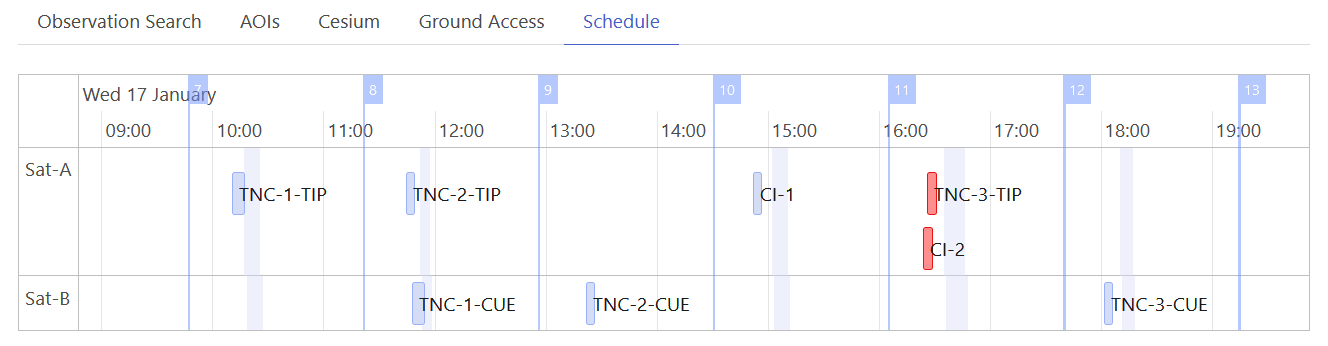
\includegraphics[width=\textwidth]{obs-conf-schedule.png} 
    \caption{Example Schedule for Plan-2}
    \label{fig:obs-conf-schedule}
\end{figure}

An example schedule can be seen in Figure~\ref{fig:obs-conf-schedule} for
Plan-2. Plan-2 was selected because there are more opportunities and there is
some time between an \gls{aoi} access and a ground access. Here, there are five
observations scheduled, 3 Tip-and-Cue Imaging observations and 2 Course Imaging
observations. The first Tip-and-Cue observation, \texttt{TNC-1-TIP}, begins at
10:10AM on Jan 17, in pass 7. Here, Sat-A begins its first tip pass over the
\gls{aoi}.  This is immediately followed by a ground contact for both
satellites with the Weilheim station. This is represented by the light grey
vertical bar.  Currently, ground contact events have not been included in the
schedule as part of an observation but this will be done in the future.  The
cue observation, \texttt{TNC-1-CUE}, happens on the next pass at 11:43AM on Jan
17.  That concludes the first observation.

While Sat-B performs the cue pass of the first observation, Sat-A begins
another observation simultaneously. Sat-B does not rely on Sat-A during a pass
so Sat-A can begin an observation as it pleases. With respect to how
observations are defined, this is acceptable, but it may conflict with the
mission's data budget. So, while the schedule does not report that there is a
conflict, in the future, another rule may be added that deals with this case.

Next, are the two Coarse Imaging Observations, \texttt{CI-1} and \texttt{CI-2},
which can be seen at 2:51PM and 4:22PM\@. The first is a legal observation but
the second conflicts with the last Tip-and-Cue observation at 4:25PM\@. The
scheduler recognizes this time conflict and highlights both events in red,
signifying to the operator that these two events must be changed before
continuing.

\subsection{Time-Tag Command Generation}\label{sec:ttc-gen}

The last stage of the \gls{pops} workflow is \gls{ttc} generation.  At this
point, the operator has created a plan that suits their own needs as well as
their customer’s needs, the plan has been validated, and all that remains is
generating \glspl{ttc} to be uploaded to their specific spacecraft.  Depending
on the observation mode, not all events have commands to be generated. In
Plan-2's schedule, commands may be only generated for the Sat-A events because
we may command it to do coarse imaging in all cases. The Sat-B events cannot
generate \glspl{ttc}. This is because for the Tip-and-Cue observation mode, on
the first pass, we may command the satellite to begin capturing wide-view
images.  But, on the next pass, we cannot command the satellite to image
potential targets as we cannot know where they will be a priori. It is known
that new commands will be generated between the first and second pass and, from
a planning perspective, this is handled with the scheduler. The time when these
inter-pass commands will be executed will lie within the second-pass event. In
this way, no other \glspl{ttc} should conflict with the automatically generated
commands because if they were scheduled for that time, they would conflict. 

To generate \glspl{ttc}, templates are combined and populated based on the
observation and the configuration parameters specified when creating the
observation. For example, one parameter may be the duration for which Sat-A
captures images. This value would then be set to an offset parameter in the
templates. 

\begin{figure}[h] 
    \centering
    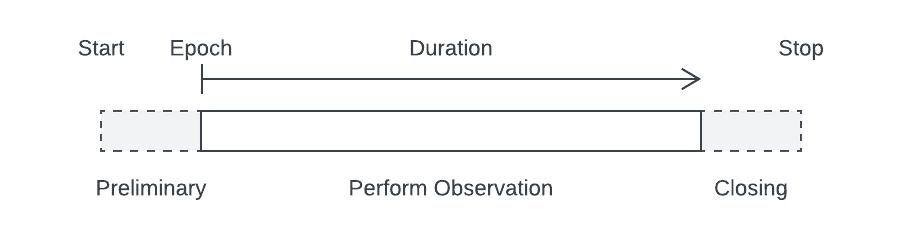
\includegraphics[width=0.7\textwidth]{timing_diagram.png} 
    \label{fig:timing} 
    \caption{Timing Diagram}
\end{figure}

The generation process is straightforward and specific to each observation mode
on each satellite. But, there are some intricacies worth noting. Firstly, when
creating an observation, the operator only specifies a duration because that is
all they are concerned with.  Generally, for any observation, there are some
preliminary and closing commands. These commands cannot happen instantaneously
and may require some non-negligible margin. It is for this reason that each
event is subdivided into separate timing components.  This can be seen in
Figure~\ref{fig:timing}. The start and stop times are the same as the event’s
start and stop but they specify when the first \gls{ttc} is executed and when
the final \gls{ttc} has concluded its execution respectively.  The epoch is the
time when the satellite begins sensing for an observation mode and the duration
is the period after which the sensing is performed. As part of the \gls{ttc}
generation capabilities, these timings can be determined programmatically by
evaluating the templates for each observation. As such, when an observation is
created by the operator in the observation configuration stage, they specify
the epoch and the duration, and the \gls{ttc} generator determines the start
and stop times. The process of generating \glspl{ttc} is still under
development and requires an intimate knowledge of the mission it is being
developed for. 





\glsresetall{} 

\chapter{Discussion and Future Work}\label{chap:discussion}

\lettrine[lines=2, findent=0pt, nindent=5pt]{A}{}t the time of writing this
thesis, the \gls{pops} is still very much in development. The project began in
2021 and has undergone continuous work since then. When designing something that
is completely unique and as ambitious as a mission planning tool, it is
difficult to gauge the work required to meet its requirements. Before,
discussing future directions for the tool, it would be helpful to first go over
how \gls{pops} became what it is. 

\section{Research and the Development Process}

Early on in development, much effort was put into exploring possible tools,
languages, and frameworks to build from. Initially, before the creation of
the Propagator service, the intention was to rely on an open-source tool,
developed by NASA, called the \gls{gmat}. \gls{gmat} is well made and designed
to model, optimize, and estimate spacecraft trajectories
\cite{hughes_using_2017}.  Originally, it was thought that it could act as a
replacement for the \gls{stk}. It could be used to take \glspl{tle} and
generate ephemerides.  \gls{gmat} comes with its own propagators and the
software could be run from the command line. Given a script representation of a
mission, ephemeris data could be generated in the form of a report.
Unfortunately, SGP4 was not supported by the software (though this was added in
a 2022 release) which made \glspl{tle} unusable given this approach.
\gls{gmat} could be expanded as it has a very well designed up plugin interface.
Theoretically, an open-source implementation of an SGP4 propagator could have
been implemented into \gls{gmat}.  Then the question arose, if a propagator
needed to be added, what was \gls{gmat} providing?  Upon evaluating this
approach, it was determined that using \gls{gmat} in this way added a great
deal of work. As well, some issues were: \gls{gmat} was restricted to a windows
environment, data needed to be transferred through a \gls{tcp} connection, and
generating mission scripts was convoluted. This is not to say that this time
was wasted; rather, this was time spent exploring a useful tool that ended up
being inadequate for \gls{sfl}'s purposes. 

%https://gmat.atlassian.net/wiki/spaces/GW/overview
%https://core.ac.uk/download/pdf/80605179.pdf

Similar work was done for another NASA tool called, OpenSPIFe. Its purpose was
to handle scheduling and planning. Very similar to \gls{gmat}, it provided a
great deal of functionality that could be updated and developed. Similarly,
this tool would have increased the amount of work for any developer working on
the project. For any tool that is used, developers must take responsibility for
it to at least understand how to use the tool but also make changes if bugs
appear. For both \gls{gmat} and OpenSPIFe, it was determined that the
development overhead for developing the tools from scratch would be far less
than having to maintain two tools, which are fully fledged projects in their
own rights developed by teams of professional software engineers.

Since the decision was made to move to develop a mission planning tool from
scratch, development became more productive than exploratory. The first service
developed was the Propagator service. Ephemeris data is fundamental to every
aspect of \gls{pops} so it was essential. Here was a situation where an
open-source library was more helpful than it was burdensome. Well tested
implementations in many languages (including Excel) of the SGP4 algorithm are
made available along with \cite{vallado_revisiting_2006}. These
implementations, though, are only of the algorithm itself and not any
surrounding functionality such as coordinate frame transforms or generating an
ephemeris. This is where a separate open-source Python implementation of SGP4
code was found. It was based on the same source code from
\cite{vallado_revisiting_2006} and it provided a library of helper functions
that enabled all of the surrounding functionality.  This allowed efforts to be
focused on validation and on using the ephemeris data rather than generating
it.

It is of the utmost importance that a developer conforms with the license
associated with a library so as to not be exposed to litigation. Most important
is whether a library requires that the source code of the software that makes
use of library must be disclosed to the public. A `copyleft' license requires
that derivative works must disclose their source code. The \gls{gpl} license is
a very common copyleft license.  Conversely, a `permissive' license makes no
obligations to derivative works. The \gls{mit} license and Apache License are
very common examples of permissive licenses.  With this in mind, time was spent
ensuring that all of the open source tools used by \gls{pops} fell under the
permissive category.  

This was especially a challenge for Cesium. Other libraries existed that
supported a 3D Earth visualization. These were basic and would require a great
deal of work to become usable. Cesium provided the most functionality with the
best \gls{api}. As such, it was worth investing time in.  Recall that CesiumJS
is the open source library that most of the functionality of the tool is built
on.  CesiumION is the proprietary version and provides 3D geospatial data which
includes world maps, terrain data, and specialized objects within the viewer.
For the world map, as long as it is cartographically accurate, it is sufficient
for \gls{sfl}'s purposes. For example, as part of \gls{pops} there is no need
for high resolution imagery of downtown Toronto.  Similarly, there is no need
for terrain data for a space application.  Time was spent looking for free
alternatives, which were found.  As such, there was no reason to pay for a
license to CesiumION when free alternatives existed.

After Cesium was made usable, most of the tools were in place to begin full
development of \gls{pops}. This began with foundational work setting up a basic
website that could be interacted with. Initially, it was very simple and had a
number of menus that could be used to create missions, add satellites, add
ground stations, and configure a plan. From this began work on the observation
configuration page which was the most complicated aspect of \gls{pops} yet
developed. It needed to interact with all the tools that had been introduced.
Not only that but it also needed to search for opportunities.

Opportunity searching was the most difficult aspect of \gls{pops}. It is
completely unique, in that there existed no open-source tool that could be
configured to find remote sensing opportunities given some constraints. Of
course, \gls{stk} could be used, but it would require a license and would need
to be automated in some way. Other tools like \gls{cpaw} could be used but
again they provided superfluous functionality and require licenses. This
process would need to be done from scratch. Before beginning development, a
document was written that fully defined all of the initial observation modes
that were desired as part of \gls{pops}. Information like: what satellites were
necessary for a particular observation; can one, some, or all be used;
explicitly defining what constraints were necessary; defining what terminology
was being used; etc. This document was then reviewed to ensure that there was a
correct understanding of what was required.

Originally, just the \gls{atu} were thought to be sufficient for opportunity
filtering. Through the creation of this reference document, it became clear
that in isolation, the \glspl{atu} could not fully constrain the observation
modes as described in the document. Strung together, they could do so.  This is
how the flow-charts similar to Figures~\ref{fig:filter-1} and
\ref{fig:filter-2} from Chapter~\ref{chap:intro} were created. They summarized,
at high level, how the \glspl{atu} could be used to fully constrain an
observation. They were easy to understand and adaptable. It followed that the
implementation of the opportunity filter should be as simple as these high
level diagrams. In response, the filter was split into a number of classes that
emulated the flow-diagrams. The Data Handler classes represented the data at
varying stages, such as: the Ephemeris, \gls{aoi}, Swaths, Polygons, and Access
Times. The \gls{atu} Handler, could use the data handler classes as inputs and
outputs. Finally, the Opportunity Filter class would use the other two classes
to fully implement a filter.  

Implementing these filters required iteration. Not just for efficiency but also
because each version made assumptions about the filters that artificially
limited the filter's capabilities.  It is very difficult to plan and account
for each aspect of the filters before-hand.  For example, the temporal
properties of the Tip-and-Cue Imaging observation had some hidden challenges.
From a high level, it is very simple: (1) first pass tip access, (2) ground
contact, and (3) next pass cue access. The initial solution may be to iterate
through each pass for a scenario. For each pass, the access time between Sat-A
and the \gls{aoi} are found. Then an access between Sat-B and the intersection
polygon from the Sat-A \gls{aoi} access is calculated. If that access exists
and if there is a ground contact, all the information is stored as an
opportunity.  This is essentially what is currently being done as outlined in
Algorithm~\ref{alg:tip-and-cue} in Chapter~\ref{chap:architecture}.  

This solution is technically valid, but what if there are multiple Sat-A
\gls{aoi} accesses in a single pass? Or, what if there are multiple Sat-B
intersection polygon accesses? Then, this process of iterating over passes may
miss potential opportunities. The solution needs to be improved and instead of
looping over every pass, the filter should iterate over every Sat-A \gls{aoi}
access.  In this way, a tip opportunity is never missed. Then, the filter
should intersect the tip intersection polygon with the first Sat-B intersection
polygon on the next pass.  This is just one example of how the process needs to
be iterated.  Other sources were effectively managing the data in a scenario.
Specifically how should data be stored such that it can be used as needed
throughout the filtering process, how to prevent copying the data
unnecessarily, or how to provide data to the \glspl{atu} effectively such that
the filter wasn't slowed down unnecessarily by performing repeated or
superfluous calculations.  

%The last area that slows down development is bug fixing and stability
%improvements. This nothing special; any part of a development workflow will
%require ironing out bugs. Given the scale of the tool, part of the attitude
%when developing has been making things perfect takes a lot of time so make it
%good enough to work for now. This is perfectly valid, and makes sense.  There
%is neither the time nor the resources to support optimizing every aspect of
%the tool. That being said, expanding the tool requires building on itself.
%Much of the functionality is inter-reliant and very little can be done in
%isolation. If we fully followed a ``get it done'' mentality, the tool would
%quickly fall in on itself. For this reason, a great deal of time has been
%spent iterating on every aspect of the tool to make it more robust, such that
%when new functionality is added, it is not limited artificially or it does not
%cause the tool to collapse in on itself.



\section{Future Work}

With some understanding for how \gls{pops} was created, some areas where
\gls{pops} needs to be developed and improved can be discussed. Some of these
are critical updates that are necessary for the \gls{mvp} and others are
important for the general health and functionality of the tool.

\subsection{Time Tag Command Generation}

The most critical aspect of \gls{pops} that must be developed is the \gls{ttc}
generation functionality. It is an essential component of the tool and cannot
be omitted. There are two aspects to this. First, the functionality for
generating \glspl{ttc} must be developed and, second, the necessary \glspl{ttc}
for each observation mode must be determined.

Work has been done to implement \gls{ttc} generation. There exists a library
developed by \gls{sfl}, written in Python, that handles the logic for creating
\gls{nsp} commands. Work was done to re-tool this library to generate
\glspl{ttc} from these \gls{nsp} commands. A service was created around the
re-tooled library to generate list of \glspl{ttc} for each observation mode.
The intention for this service was to be expandable and easy to use for future
developers since what \glspl{ttc} are used for each observation mode will
change from mission to mission. This where the intricacies discussed in
Section~\ref{sec:ttc-gen} where discovered.  

Unfortunately, it was decided that using Python scripting to generate
\glspl{ttc} may be too complicated or cumbersome for future developers. In
addition, the \gls{nsp} library did not explicitly track the data payloads of
the \gls{nsp} commands. That is, the library could construct valid commands but
they did not track mission-specific information. For example, if a command were
to be sent to the \gls{hkc} on the satellite and the \gls{hkc}'s address was
\texttt{0x06}, the developer would have to write the address itself within the
code. This makes development more difficult since a developer would need to
understand the commands themselves, rather than having that functionality be
handled by the software. 

Typically, for ground software at \gls{sfl} this is handled by \gls{xml}
configuration files that are configured for each new mission.  The \gls{nsp}
library did not make use of these configuration files because it was made for
testing and not necessarily for nominal operations. So, when using the Python
\gls{nsp} library, individual data bits would need to be specified in
Hexadecimal.  Despite the amount of work put into this new service, it was
decided that these issues were irreconcilable with the future needs of
\gls{pops}. So, the service was replaced by a new tool that builds off
\gls{xml} configuration files as the foundation for \gls{ttc} generation.  This
tool is still in development.

Determining what commands are necessary for each observation mode is difficult.
Necessary commands may be: powering on devices in the spacecraft, setting
profiles, arming and disarming these profiles, specifying where in memory where
data should be stored, specifying the necessary duration for commands,
specifying attitude modes, etc.  There does not exist a single reference for
what commands are necessary and what must be done for an observation mode. This
information can only be gained through discussion with operators and with
software engineers developing the firmware.  Even after extensive consultation,
there is potential for steps being missed. It is only through testing, are all
of the necessary commands for an observation mode determined.  Thankfully, much
of this testing can be done during \gls{tvac} testing campaigns. It is here,
were spacecraft may be commanded to perform observations, or at least their
ground analogues, through \glspl{ttc}.  This gives a great deal of information
about what specifically needs to be performed for each observation. It also
provides some means of validating \gls{ttc} generation.


\subsection{Validation}

The next most important aspect of \gls{pops} that must be accomplished before
an \gls{mvp} is ready, is validation. The tool must yield acceptable and
accurate results. System level validation can be accomplished through
service-level verification. This has been touched on throughout the thesis.
Specifically, the Propagator service was validated through comparing ephemeris
data with results from \gls{stk}. \gls{ttc} generation validation may be
accomplished through \gls{tvac} testing. After this, validation becomes
difficult. The \glspl{atu} may must be individually validated either through
known test cases or through comparisons with \gls{stk}. This process has been
handled separately.  Opportunity filtering is especially difficult to validate
since there does not readily exist an alternative that can act a benchmark. In
the future, what may be done is when the filtering process has reached
maturity, simple test scenarios will be constructed for each observation mode.
\gls{stk} and \gls{pops} will separately be used to search for opportunities
and these results will be compared. Thankfully, there is not a requirement for
some of the components. For example, a high accuracy with respect to access
times is not necessary. Even if the access time calculation were made very
accurate, there are inherent uncertainties in the ephemeris data that may
render such accuracy useless. Developing validation strategies is an ongoing
process.
 
%\subsection{Addition of More Observation Modes}
%
%Some missions that \gls{pops} is intended to be used for require additional
%operations modes beyond just what was discussed in the 

\subsection{Performance}

Currently \gls{pops} has issues with large amounts of data. For scenarios
longer than a few days, storing and retrieving data, displaying information,
and opportunity filtering becomes slow. To illustrate this, let us run a simple
benchmark test. For this test, we will run the Tip-and-Cue Imaging opportunity
filter for a number of scenarios, each with an increasing scenario size and a
10s timestep. Each scenario will have two satellites (Sat-A and Sat-B), three
ground stations (\acrshort{sfl}, ESCS, and GSW), and the same \gls{aoi}
discussed in Chapter~\ref{chap:workflow}. The reason we'll use the opportunity
filter as a benchmark is that it interacts with almost every part of \gls{pops}
and Tip-and-Cue Imaging is the more complicated observation mode.
The purpose of this test is not to give an in-depth characterization of the
performance of \gls{pops} but rather its purpose is to give a rough idea of its
potential.  These scenarios were run on a laptop with 40GB of RAM and an
$11^{th}$ generation Intel Core i7-1165G7 CPU running at 2.80 GHz. 


\begin{figure}[h]
    \centering
    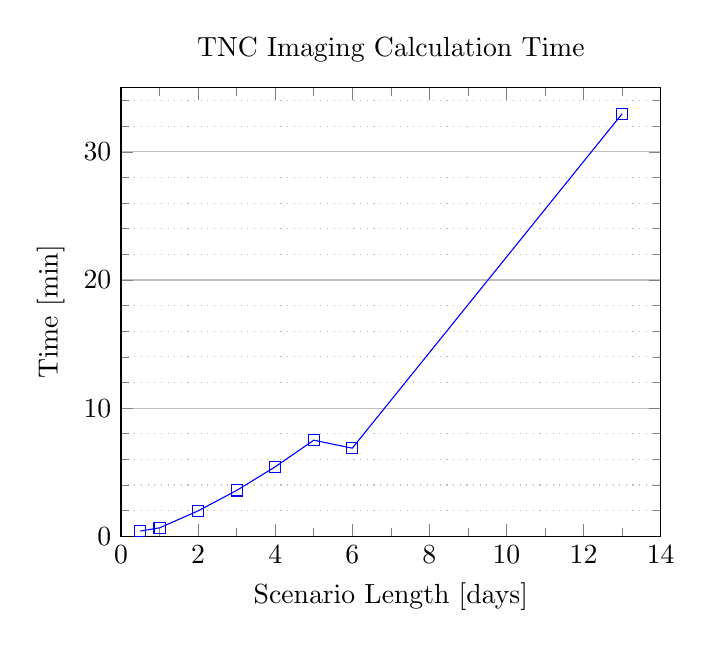
\begin{tikzpicture}
    \begin{axis}[
	title={TNC Imaging Calculation Time},
	xlabel={Scenario Length [days]},
	ylabel={Time [min]},
	xmin=0, xmax=14,
	ymin=0, ymax=35,
	xtick={0, 2, 4, 6, 8, 10, 12, 14},
	minor x tick num=1,
	minor y tick num=4,
	ymajorgrids=true,
	yminorgrids=true,
	minor grid style=dotted,
    ]

    \addplot[
	color=blue,
	mark=square,
	]
	coordinates {
	(0.5, 0.400643333) (1, 0.651415) (2, 1.976971667) (3, 3.57072) (4, 5.415478333) (5, 7.492456667) (6, 6.871896667) (13, 32.980525)
	};
	
    \end{axis}
    \end{tikzpicture}
    \caption{Simple Opportunity Filtering performance benchmark}
    \label{fig:performance-benchmark}
\end{figure}

The results of this test can be seen in Figure~\ref{fig:performance-benchmark}.
As can be seen from the plot, 8 scenarios were generated. Scenarios less than 4
days are reasonably quick, taking less than $\sim5$ minutes. But, as we
approach a 13-14 day scenario filtering takes more than half an hour. It could
be argued that this is tolerable for an \gls{mvp} but it is certainly not
ideal.  Note, this test was only for a 2-satellite scenario. Every satellite
added increases the running time exponentially. 

To address this, there are a number of areas for improvement to consider.
These range from simple algorithmic changes to heavily involved architectural
changes. For each change, work will need to be done characterizing what is
taking up the most time to justify the change. Some possible avenues for
improvement, in increasing difficulty, are:

\begin{enumerate}
    \item Making ephemeris data dynamic,
    \item Splitting up the data in the filtering process,
    \item Utilizing parallel computation,
    \item Offloading computation to a dedicated server, or
    \item Leveraging the GPU
\end{enumerate}


\subsubsection{1. Making Ephemeris data dynamic}

Ephemerides are generated for each satellite once when a plan is created. This
ephemeris data has a set time range and timestep. It is here a user must decide
whether they want an accurate but slow to process plan, or an inaccurate but
fast plan. Why should they be required to make this decision? Or, at least, why
should this decision be made once and then be set in stone for the duration of
the plan? What's more, if the timestep is constant for an entire plan, it is
likely that, for small timesteps, most of that data is wasted. If a user is
concerned with an \gls{aoi} in the Northern Hemisphere, they will not need a
high accuracy ephemeris for times where the spacecraft is in the southern
hemisphere. Of course, if the user is concerned with a very large \gls{aoi}
that the spacecraft more often than not has access to, then nothing can be
done. This, though, is an outlier case.

This touches on potential improvements for how ephemerides can be better
handled.  Instead of initially making a large ephemeris with a small timestep,
a rougher, large timestep, ephemeris could be generated.  For periods where
high accuracy is needed, such as when there is an access, ephemeris data could
be dynamically generated in that area specifically to increase the accuracy
where it is needed. Or, conversely, a small timestep ephemeris could be
initially generated, then after the calculations are performed, unnecessary
data could be omitted. These are both general ideas for now and would need
dedicated development time to plan out and troubleshoot any pitfalls.

In terms of difficulty, this would require a re-work of a large portion of
\gls{pops}.  Thankfully, through abstracting how ephemeris data is handled
through the Data Handler classes, \gls{pops} is well situated for this change.
Overall, this is a change that will likely be made later.  Having ephemeris
data be static artificially limits \gls{pops}'s functionality.


\subsubsection{2. Splitting up data in the filtering process}

Currently, during opportunity filtering, all of the data is loaded for the
entire scenario. That being ephemeris data, swaths, access times, etc. If
having all of this data loaded in at once is causing the filtering process to
slow down, it may be better to instead load the data in chunks. For example,
for a 14 day scenario, instead of loading in all 14 days of data, this could be
split up into 2 day chunks. This will likely not reduce the processing time but
it may reduce the time spent indexing and accessing the data. In terms of
difficulty, this would be an easy modification but time would need to be spent
determining whether this change is worthwhile.


\subsubsection{3. Utilizing parallel computation}

Moving from single-threaded processing to multi-threaded processing begins to
stray from algorithmic changes to a change in how the host PC is utilized.
These solutions, while most likely effective, increase the complexity of
\gls{pops} and should be pursued if there are no other alternatives.

Thankfully, opportunity filtering is well suited for multi-threaded
programming. Searching for opportunities is done through brute-force numerical
computation, and many of the calculations are performed independently from each
other. A system could be developed that splits the filtering process into a
number of processes, each handling sub-components of the filtering process. 

This would be a difficult solution to implement. Multi-threaded programming is
not necessarily complicated in Python, but asynchronous processes are almost
always much more complicated than asynchronous process. Synchronous processes
are predictable, straightforward, and easy to debug. Asynchronous processes are
none of these and introduce a multitude of challenges. For example: race
conditions, memory management, locking out resources, unpredictable behavior,
error handling, etc.  There are many benefits to parallel computing, but such a
change should not be undertaken lightly.


\subsubsection{4. Offloading computation to a dedicated server}

When performing opportunity filtering, or any other function of \gls{pops}, if
other software is being run on a user's computer, that may negatively impact
the tool's performance. Or, if the user's computer is not particularly
powerful, that may limit \gls{pops}'s usefulness. Instead, a dedicated server
could be constructed that is optimized to perform calculations for \gls{pops}.
Some calculations may be: ephemeris generation, the \glspl{atu}, database
management, and opportunity filtering. In this way, all that a user's computer
will run is what they need to display the information or construct requests.
Alternatively, all of \gls{pops} could be hosted on a server, and a user could
access it completely remotely. 

There are potential benefits to this approach, but it would vastly increase the
complexity of \gls{pops}, especially for the front-end user interface. Some
difficulties would include: managing data transfer, tracking user sessions, or
potentially removing functionality from the Mission Model service. The issue of
tracking user sessions is particularly difficult. If a user runs \gls{pops} on
their own computer, it can be assumed that only they will be interacting with
the webserver. But, if the server is hosted remotely, then the webserver needs
to track both what requests are being sent to it as well as from what source.
For example, let us say there are two users who wish to work with two different
plans. User 1 will open Plan A and the webserver will display Plan A. User 2
will open Plan B and Plan B will be displayed. Suppose then User 1 makes a
change to Plan A, the webserver will receive the request but, since it isn't
tracking from what source are the requests coming from, it will make changes to
Plan B since that was the last plan displayed.  The behavior is undefined and
both User 1 and User 2 will have unstable sessions.  In this way, sessions
should be split somehow, such that one user's inputs cannot affect another
user. This problem has many solutions but is non-trivial and strays into
professional web development which is not the priority for \gls{pops}. 


\subsubsection{5. Leveraging the GPU}

So far, all computation has been done on the \gls{cpu} which is general purpose
but slow. The \gls{gpu} is optimized for computer graphics and image
processing. Specifically, they are built to process large blocks of data in
parallel. They are especially good at handling any process that uses linear
algebra. Historically, \glspl{gpu} were only meant to be used for computer
graphics but recently, they have become much more general purpose. By
leveraging the \gls{gpu}, computation times may be decreased by orders of
magnitude. Some precedent does exist for this by accelerating SGP4 calculation
\cite{moeckel_high_2016} \cite{fraire_opencl-accelerated_2013} and it is
reasonable to assume this can be expanded further.

Using a \gls{gpu} would be the most rewarding but also most difficult and
complicated improvement to \gls{pops} that could be made. Writing code for a
\gls{gpu} is to some extent specific to the manufacturer and age of the
\gls{gpu}. Some computers that may run \gls{pops} may not even have a \gls{gpu}
that supports this functionality. So in addition to creating the custom shaders
for \gls{pops}, work would need to be done to ensure that they can be used by
users at \gls{sfl}.
 

\subsubsection{Miscellaneous Improvements}

In addition to any large improvements, there exists many smaller changes that
can have a positive effect on \gls{pops}'s performance. Small changes such as:
dynamically loading data from the database, sending multiple batches of data to
the \glspl{atu} in a single HTTP request rather than multiple HTTP requests, or
optimizing data formats based on need.


\subsection{Updating Plans}

Another area that must be improved is the ability to update plans in
\gls{pops}. Currently, once \glspl{tle} are set for a plan, they cannot be
changed. This was done to reduce the complexity of the tool but this is not an
ideal solution.  Suppose a plan has been made and observations have been
scheduled, but then suppose after some time a new \gls{tle} is generated that
invalidates the observations made with the older \gls{tle}. This is a
reasonable scenario that could very well occur but currently there is no way to
handle this in \gls{pops} aside from creating a new plan and rescheduling
observations.

This is a multi-faceted problem that must be addressed in a number of areas.
First, it must at least be determined if a new \gls{tle} invalidates
observations from a plan with a previous \gls{tle}. Next, there must be a way
to edit observations in an old plan or there must be a way to migrate those old
observations to a new plan with updated timings. Lastly, if a change is made to
an observation, \glspl{ttc} that have already been generated must be updated in
some way to reflect those changes. This problem has not yet been approached and
is an on-going limitation of the tool.


\subsection{Communication With Other Ground Software}

\gls{pops} is not meant to be used in isolation. It is important that it is
able to communicate with other ground software at \gls{sfl}. Specifically,
\gls{pops} must be able to read commands that are scheduled for different
spacecraft. This is necessary for planning and scheduling.  Without an
understanding of what is already planned for a satellite, observations that a
user adds may conflict with existing \glspl{ttc}.  How exactly \gls{pops} will
interact with \gls{sfl}'s ground software has yet to be determined.  

This additional functionality is planned to be an additional class which acts
as an interface between the scheduler class and \gls{sfl}'s ground software. It
is here uploaded \glspl{ttc} will be read and added onto the schedule.



\subsection{Testing}

The last task that must be performed before \gls{pops} has reached the
\gls{mvp} is user testing. Quite simply, this is where operators begin to use
the tool and give feedback. This information is critical since it gives insight
into: bugs, user interface problems, and what parts of the tool can be
improved.  This then begins the process of iterating in their feedback,
improving the tool, receiving further feedback and so on.


         
\glsresetall{} 

\chapter{Conclusion}\label{chap:conclusion}

%\lettrine[lines=2, findent=0pt, nindent=5pt]{T}{} 

This thesis has discussed the purpose, design, and implementation of the
\gls{pops} developed by the \gls{sfl}. \gls{pops} is being developed to address
the need for mission planning capabilities for the operations at \gls{sfl}. It
is not intended to fully automate an operator's workflow but rather its purpose
is to streamline some of their day to day activities. The main design direction
for this tool has been to keep it easy to use and easy to develop. Many tools
have been developed at \gls{sfl} that have fallen into obscurity.Further, even
if a tool is very efficient, this is less valuable than a tool that can be
expanded into the future. 

Existing software solutions to mission planning that are currently available
have been introduced. Their strengths as well as their weaknesses have been
discussed. After this some terminology was introduced as well as some
operations related concepts. Since it is not the desire of the author to expose
the operations strategies of \gls{sfl} customers, an example scenario was
defined, EG-SAT, to illustrate the usefulness of \gls{pops}.

After this, the architecture of \gls{pops} was discussed, starting with the
general architecture of the software. Then going into the specifics of each
service, those being the: Propagator, Database, Access Time Utilities, and
Mission Model. The propagator generates validated ephemeris data. The Database
persistently stores mission and search data. The Access Time Utilities serve as
the basic building blocks from which opportunities may be filtered from search
data. Lastly, the Mission Model is the heart of the tool.  It handles the
front-end user interface, communication with the database, opportunity
filtering, data handling, and event scheduling.

Just discussing the architecture does not fully explain the purpose of
\gls{pops}. To help aid in this process, a workflow was discussed for the
EG-SAT mission. Starting with setting up \gls{pops} for a mission, adding
satellites, and ground stations. After this, a plan was set up for a 3-day
period. There, opportunities were searched for given EG-SAT's two operations
modes, Coarse Imaging and Tip-and-Cue Imaging. From these opportunities,
observations were created and added to the schedule. The schedule was then
validated and displayed.  

Lastly, future work for \gls{pops} was discussed. This included required
funcitonality, validation and testing, as well as potential performance
improvements.

%the research and development process was discussed. What tools were
%originally used and what they were replaced by. As well, the process for
%developing the opportunity filter was discussed. After this some avenues for
%improvement were explored for \gls{pops}. 

A great deal of work lies ahead for \gls{pops} but this is only a testament to
the amount of work that has already been accomplished. Hopefully, this tool
will provide some benefit to operators at \gls{sfl} for many years to
come.










           
\glsresetall{} 
\appendix

\chapter{Algorithms} \label{chap:Algorithms}

%\lettrine[lines=2, findent=0pt, nindent=5pt]{T}{} 

Through the development of the \gls{pops}, a number of algorithms have been
developed to perform various functions. These algorithms are not necessarily
ground breaking but their implementations are novel and worth discussing in
some form. To avoid detracting from the main body of the thesis they are
discussed here, in the appendix.


\section{Multiple Access Intersection Algorithm} \label{alg:mul-access-inter}

For some search scenarios, \gls{pops} may need to determine for what times do all
satellites have access to a target such as an \gls{aoi} or a ground station.
That is, if there are multiple satellites and each satellite has a list of
access times to a target, \gls{pops} must generate a new list of access times where
each access corresponds to a period where all satellites have access. An
example scenario is illustrated in Figure~\ref{fig:access_intersect}.


\begin{figure}[h]
    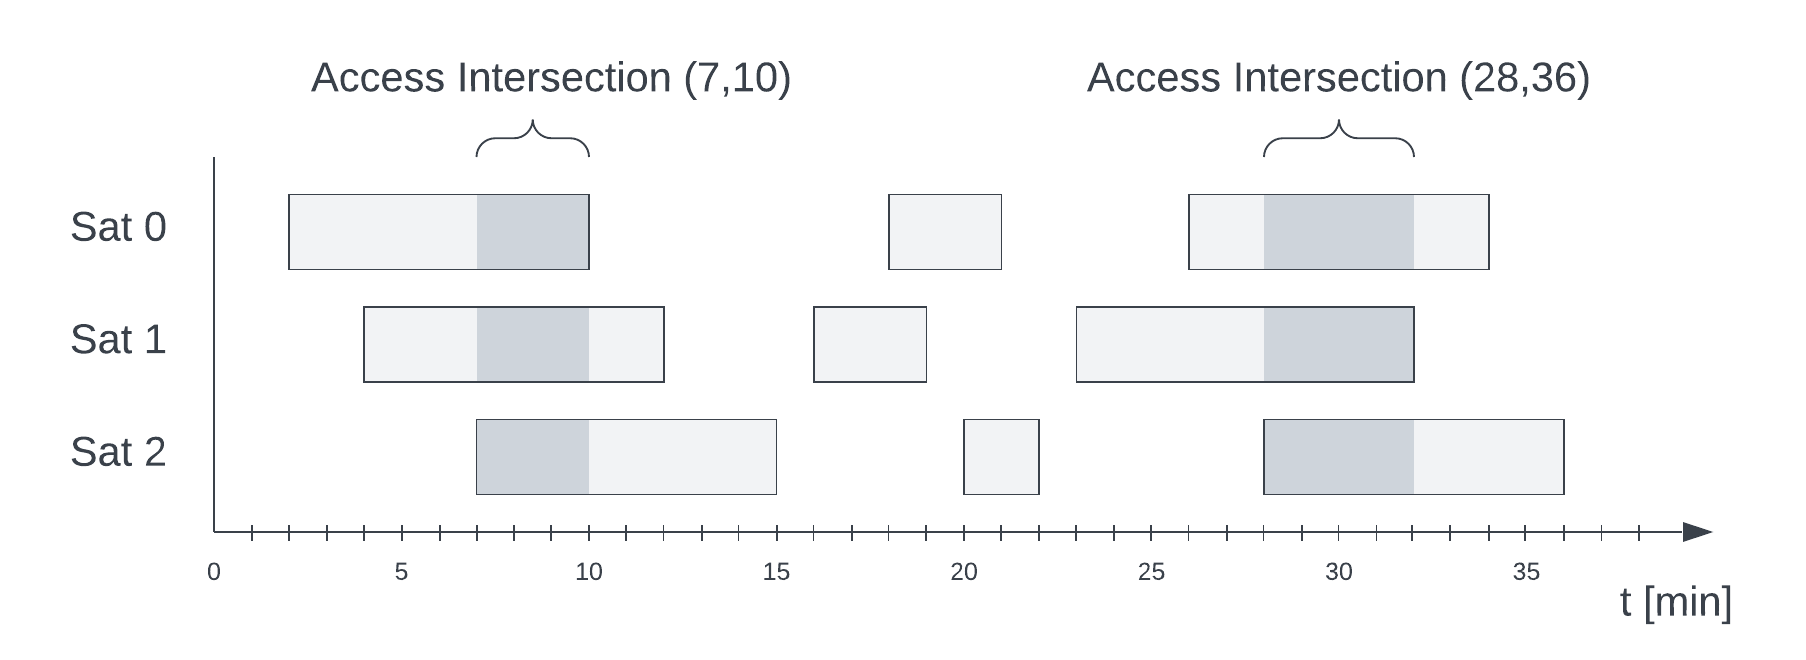
\includegraphics[width=\textwidth]{Access Intersection Example.png} 
    \caption{Illustration of a Potential Access Intersection Scenario}
\label{fig:access_intersect}
\end{figure}

In this scenario, there are three satellites: Sat 0, Sat 1, and Sat 2. Each has
multiple access periods represented with gray boxes. Though time is continuous,
it has been discretized into integer timesteps for simplicity. Minutes have
been selected as the units for time but this is arbitrary. From these lists of
access periods, this algorithm must determine all of the points in time where
all satellites have an access period. For the example scenario, the outputted
results should be $[7,10]$ and $[28,36]$. Note that between $t = 16$ and $t=22$
there are access overlaps but since there are only overlaps between two
satellites, they should not be returned as intersection periods.

For each satellite, access times are stored as a list of timestamps. Every even
and odd indexed timestamp specifies when the satellite `enters' and `leaves' an
access respectively. Access lists $\ses{a}{n}$ can be described generally for
satellite $n$ as,

\begin{equation}\label{eq:access-list} 
    \ses{a}{n} = \left[ a_{n,0}, b_{n,0}, a_{n,1}, b_{n,1}, \ldots a_{n,m}, b_{n,m} \right]
\end{equation}


where $a$ is the access enter timestamp, $b$ is the access leave timestamp, and
$m$ is the number of accesses. We also make the assumption that no accesses
overlap for a given satellite and target; that is,

\begin{equation}\label{eq:access-list-constraint}
    a_{n,0} < b_{n,0} < a_{n,1} < b_{n,1} < \ldots < a_{n,m} < b_{n,m}
\end{equation}

One simple brute force solution to this problem would be to iterate over every
time step, $t$, and check if there exists an access region, $[a_n,b_n]$, for all
satellites, $n$, such that $t$ is between $a$ and $b$.

This solution is, of course, very wasteful as it scales with the number of
timesteps that are being considered, $\Theta(t)$. The number of timesteps may
be on the order of 1,000s to 10,000s of timesteps. A simplification can be made
since we do not need to actually consider every timestep. Rather, we can
instead iterate over the access boundaries since they describe continuous
periods of time. By focusing on just the access boundaries, we may develop an
algorithm which scales with the number of accesses, $\Theta(m)$, which is much
smaller than the total number of timesteps.

For all satellite access lists we are considering, let us combine them into two
$1\times nm$ arrays. The first `timestamp' array, $\se{b}$, contains a sorted
list of all of the boundary timestamps in ascending order. The second `index'
array, $\se{s}$, contains a list of satellite indices in the same order as the
timestamp array. For example,

\begin{equation*}
    \begin{aligned} 
	\ses{a}{0} &= \left[ 2, 10, 18, 21  \right] \\
	\ses{a}{1} &= \left[ 4, 12, 16, 19  \right] \\
	\ses{a}{2} &= \left[ 7, 15, 20, 22  \right] \\
    \end{aligned}
    \quad \Rightarrow \quad
    \left \{ 
	\begin{aligned}
	    \se{b} &= [ 2 , 4 , 7 , 10 , 12 , 15 , 16 , 18 , 19 , 20 , 21 , 22  ] \\
	    \se{s} &= [ 0 , 1 , 2 , 0 , 1 , 2 , 1 , 0 , 1 , 2 , 0 , 2  ]
	\end{aligned}
    \right.
\end{equation*}

Note these are some of the values from Figure \ref{fig:access_intersect}.
Again, in the actual implementation of the algorithm we use actual timestamps
but here we are using integers for demonstration purposes. The timestamp array
stores the timestamp of the access boundary for later reference and also gives
us the order of the satellite index array. Remember that access boundaries are
listed in order of [enter, leave, enter, leave, ...]. Looking at the first four
elements in the index array, $[0, 1, 2, 0]$, satellite 0 enters an access at
the first element and leaves the access at the fourth element. So for the
second and third element, satellite 0 still has access because it has not left
yet. In essence, the index array encodes in what order satellites enter and
leave accesses. 

Now let us expand on the index array so we can perform logical operations to
find intersections. For this the algorithm makes use of logic arrays.  These
are arrays which contain only Boolean values, True or False. With these arrays,
we can also perform logical operations on any axis. For example, if we have a 2
dimensional logic array, we can produce a 1 dimensional array, that is the
result of AND'ing all of the elements in each column. These allow us to perform
logical operations very quickly for many elements. From the index array let us
construct an $n\times nm$ boolean array, $\se{A}$, that describes our scenario.
The rows of matrix, $\se{A}$, correspond to the indices of each satellite.  For
example row 0 is satellite 0, row $m$ is satellite $m$, etc. The columns
correspond to elements in the index array, $\se{s}$.

Let us initialize $\se{A}$ to be all False values represented as 0s. Then,
starting at the first column of $\se{A}$, let us NOT the element in the
$\se{s}(0)$ row.  Then, for then next column, let us copy all of the values
from the previous column and again NOT the $\se{s}(1)$ element. This is then
repeated for all columns in $\se{A}$. There is one small catch, if we are
transitioning a 1 to a 0 or a True to a False, this should be done on the
following iteration. This essentially means that we are treating accesses in in
access boundaries as inclusive. Even if the satellite is leaving an access, we
say that it has access until the timestep immediately after the boundary. As an
example, let us construct $\se{A}$ from $\se{s}$ for all of Figure
\ref{fig:access_intersect},

\begin{equation*} 
    \se{s} = 
    \left[
    \begin{array}{cccccccccccccccccc}
	0 & 1 & 2 & 0 & 1 & 2 & 1 & 0 & 1 & 2 & 0 & 2 & 1 & 0 & 2 & 1 & 0 & 2 \\
    \end{array}
    \right]
\end{equation*}
yields,
\begin{equation*} 
    \se{A} = 
    \left[
	\begin{array}{cc;{2pt/2pt}cc;{2pt/2pt}cccccccccc;{2pt/2pt}cc;{2pt/2pt}cc}
	1 & 1 & 1 & 1 & 0 & 0 & 0 & 1 & 1 & 1 & 1 & 0 & 0 & 1 & 1 & 1 & 1 & 0 \\
	0 & 1 & 1 & 1 & 1 & 0 & 1 & 1 & 1 & 0 & 0 & 0 & 1 & 1 & 1 & 1 & 0 & 0 \\
	0 & 0 & 1 & 1 & 1 & 1 & 0 & 0 & 0 & 1 & 1 & 1 & 0 & 0 & 1 & 1 & 1 & 1 \\
    \end{array}
    \right]
\end{equation*}
Then, if we AND all of the rows in $\se{A}$ we get,
\begin{equation*} 
    \se{A}' = 
    \left[
    \begin{array}{cccccccccccccccccc}
	0 & 0 & 1 & 1 & 0 & 0 & 0 & 0 & 0 & 0 & 0 & 0 & 0 & 0 & 1 & 1 & 0 & 0 \\
    \end{array}
    \right]
\end{equation*}
It is clear to see that this matrix gives us the indices where there is an
intersection between all satellites. If we take all values of $\se{b}$ where
$\se{A}'$ is True, we are left with,
\begin{equation*} 
    \se{b}' = 
    \left[
    \begin{array}{cccccccccccccccccc}
	7 & 10 & 28 & 32
    \end{array}
    \right]
\end{equation*}
which is our expected result. This was just a walkthrough but the explicit
algorithm definition is defined in Algorithm~\ref{alg:access-intersection}.

\begin{algorithm}[h] 
    \caption{Access Intersection} 
    \label{alg:access-intersection}
    \begin{algorithmic}[1]
	%\Require{\se{z}is a $1\times N$ array } 
	\Function{AccessIntersection}{$\ses{a}{0}$,$\ses{a}{1}$, ... , $\ses{a}{n}$} 

	    \Let{$\se{s}$, $\se{b}$}{\Call{Combine}{$\ses{a}{0}$,$\ses{a}{1}$, ... , $\ses{a}{n}$}}  

	    \Let{$l$}{\Call{Length}{$\se{s}$}}

	    \Let{$\se{A}$}{\Call{Zeros}{$n$,$l$}}

	    %\Let{$\se{A}[\se{s}[0],0]$}{1}  \Comment{Set up the first column}
	    \Let{$\se{t}$}{$\se{A}[:,0]$} \Comment{Temporary array to store column of $\se{A}$}

	    \Let{$i$}{0} \Comment{Boundary iterator}

	    \While{$i \neq m$}
		\Let{$s$}{$\se{s}[i]$} \Comment{Satellite index}
		
		\If{!$\se{t}$($s$)}
		\Let{$\se{t}$($s$)}{!$\se{t}$($s$)}
		    \Comment{Flip element then copy values over}
		    \Let{$\se{A}[:,s]$}{\Call{OR}{$\se{A}[:,s]$, $\se{t}$}} 
		\Else
		    \Let{$\se{A}[:,s]$}{\Call{OR}{$\se{A}[:,s]$, $\se{t}$}} 
		    \Comment{Copy values over then flip element}
		    \Let{$\se{t}$($s$)}{!$\se{t}$($s$)}
		\EndIf


		\Let{$i$}{$i+1$}
	    \EndWhile 

	    \Let{$\se{a}'$}{\Call{ColumnsAND}{$\se{A}$}}

	    \Let{$\se{b}'$}{$\se{b}[\se{a}']$} \Comment{Select indices based on logical value}

	\State \Return $\se{b}'$
	\EndFunction
    \end{algorithmic}


\end{algorithm}

For this algorithm, the implementation of \textsc{Combine} function was omitted
for clarity since it is an implementation detail. Also, note that this
algorithm is not limited to only access intersections but it may also calculate
unions by replacing \textsc{ColumnsAND} with \textsc{ColumnsOR} in line 18.

%%%%%%%%%%%%%%%%%%%%%%%%%%%%%%%%%%%%%%%%%%%%%%%%%%%%%%%%%%%%%%%%%%%%%%%%%%%%%% 

%\section{Equator Crossing Algorithm} \label{sec:equator-crossing}
%
%For a given ephemeris, it is useful to determine each `pass' of that orbit.
%That is, for each ephemeris point, an index should be assigned to it which
%indicates how many times the spacecraft has orbited the Earth. In this way, if
%we have some time range and we wish to see the next `pass,' we would simply
%take that time range's pass index and add 1.
%
%There are many ways a pass may be defined. For example, we could specify a
%latitude and longitude range and whenever the spacecraft is in this range, that
%could be considered a singular pass.  Generally, though, ephemeris data is not
%given in latitude or longitude, rather it is given in a Cartesian position in
%some \gls{eci} or \gls{ecef} coordinate reference frame. So, for each position
%in the ephemeris, the position vector will need to be converted to latitude and
%longitude. 
%
%This is a completely acceptable approach but we may also simplify the problem.
%Instead of taking a latitude and longitude range, we could instead increment
%the pass index when the spacecraft crosses the equator and goes from the
%southern to the northern hemisphere. This would be when the spacecraft's
%position goes from a negative to a positive latitude. This definition of a pass
%has a few advantages. That being, we only need to do one check to determine a
%pass boundary. It also has the benefit of indexing the entire ephemeris. Still
%for this method, we need to convert from Cartesian position to at least
%latitude.
%
%Let us make one further simplification by assuming that the x-y plane of the
%ephemeris's coordinate system is very near to the Earth's equatorial plane.
%This is not true for all coordinate systems but it is true for the \gls{ecef}
%ephemerides used by \gls{pops}. By making this assumption, we no longer need to
%calculate the latitude of the spacecraft; rather, we can instead only look at
%the spacecraft's position along the z-axis. This is useful because the
%spacecraft's z-position will oscillate between some positive and negative
%extrema, which are determined by the orbit's inclination and eccentricity. 
%
%There is a complicating factor that should be accounted for. In time, the
%spacecraft's position is periodic, but when considering only the spacecraft's
%z-position in an ephemeris, there is no guarantee that there is a constant
%timestep between position values. Additional data-points may be injected for
%periods where greater accuracy is desired and vice-versa. 
%
%We may now articulate the problem to be addressed: Given, an array of
%$z$-positions, $\se{z}$, generate a new array, $\se{p}$, that each element of
%$\se{p}$ is the index of an element in $\se{z}$ after a crossover occurs (i.e.\
%the positive value in the negative-to-positive crossing). To determine if
%elements, $n$ and $m$, of an array, $\se{z}$, form a crossover, they must
%satisfy three simple conditions:
%
%\begin{enumerate}
%    \item $\se{z}[n] < 0$
%    \item $\se{z}[m] > 0$ 
%    \item $m = n+1$
%\end{enumerate}
%
%
%A brute-force approach to finding $\se{p}$ would be to loop through all of the
%elements in $\se{z}$ and test them against the above conditions. This method,
%though, is inelegant and may be computationally intensive.  
%
%Alternatively, we can instead try and make use of 
%
%Another approach to
%this problem is outlined in Algorithm~\ref{alg:crossover}.  In essence, it
%attempts to reduce the number of comparisons made to search for crossovers. 
%
%\begin{algorithm}[h] 
%    \caption{Negative-Positive Crossing Search Algorithm} 
%    \label{alg:crossover}
%    \begin{algorithmic}[1] 
%	\Require{\se{z}is a $1\times N$ array } 
%
%	\Function{FindAllCrossovers}{$s, f, \se{z}$}
%	    \Let{$p$}{\Call{FindNextCrossover}{$0, s, f, \se{z}$}} \Comment{Start at beginning of array}
%	    \Let{$\se{p}$}{$\{ p \}$}
%
%	    \While{$p \neq -1$}
%		\Let{$p$}{\Call{FindNextCrossover}{$p, s, f, \se{z}$}}
%		\Comment{Start at beginning of array} \State
%		$\se{p}$.append($p$) \EndWhile 
%		\State \Return \se{p}
%	\EndFunction
%
%	\State
%
%	\Function{FindNextCrossover}{$i, s, f, \se{z}$} 
%	\Let{$j$}{$i+s$}
%	\If{$j > length(\se{z})$} 
%	    \State $s = \mathrm{s \times f}$  
%	\ElsIf{$j = length(\se{z})$}
%	    \State \Return $-1$	  \Comment{Search has completed}
%	\ElsIf{ $(\se{z}[i] < 0) \lor (\se{z}[j] > 0)$ }
%	    \If{$s=1$}
%	    \State \Return $i$ \Comment{Crossover index found}
%	    \Else
%		\State $s = ceil(s \times f)$
%	    \EndIf
%	\Else
%	    \State $i=j$
%	\EndIf
%	\State \Return \Call{FindNextCrossover}{$i, s, f, \se{z}$}
%	\EndFunction 
%    \end{algorithmic} 
%\end{algorithm}


%%%%%%%%%%%%%%%%%%%%%%%%%%%%%%%%%%%%%%%%%%%%%%%%%%%%%%%%%%%%%%%%%%%%%%%%%%%%%% 

\section{Single Access Intersection Algorithm} \label{alg:contains}

The Single Access Intersection Algorithm is similar to the Multiple Access
Intersection algorithm but it serves a different purpose. Given a time range,
this algorithm is concerned with finding all of the access times in a list that
intersect that time range. Here, the input time range will not be used as
bounds, but only search criteria to select access times. 

\begin{figure}[h]
    \centering
    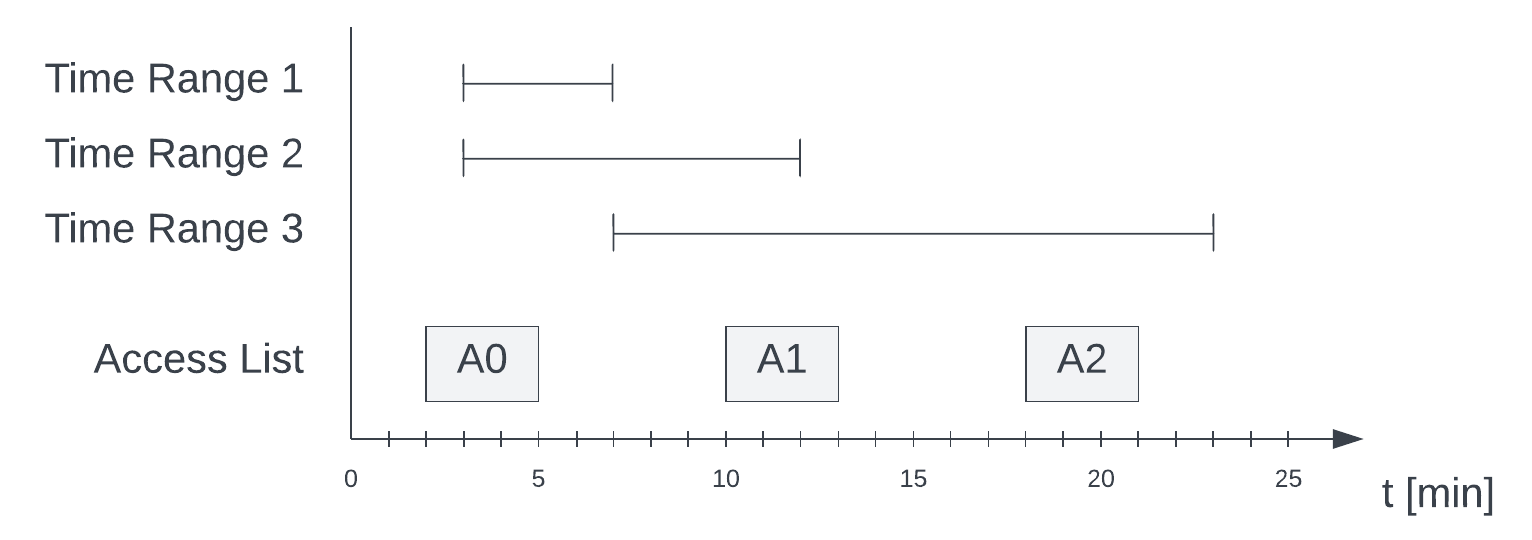
\includegraphics[width=\textwidth]{Single Access.png} 
    \caption{Illustration of a Potential Single Intersection Scenarios}
    \label{fig:single-access-intersect}
\end{figure}

To get a better idea of the problem, let us look at some more concrete example
scenarios. Figure~\ref{fig:single-access-intersect} illustrates an access list
as well as three possible input time ranges, time range 1-3. For time range 1,
the output should be merely A0. For time range 2, the output will be A0 and A1.
Lastly, time range 3 will have outputs A1 and A2. Notice here that the limits
of the time range may lie within or without an access. As long as the access
intersects the time range at all, it should be included.

The two inputs to this algorithm are a time region with boundaries $\alpha$ and
$\beta$ where $\alpha < \beta$. The access list, $\se{a}$, is the same as
described in Equation~\ref{eq:access-list} where the subscript, $n$ has been
omitted since only one access list is to be considered. Additionally, the
assumption in Equation~\ref{eq:access-list-constraint} still holds here. It
should be emphasized that given an access list, every even entry is an access
enter timestamp and every odd entry is an access leave timestamp.

The main intuition for this problem is that we must first constrain the list of
access boundaries to the those boundaries that lie within the time range.
Then, we must assemble the access times from their boundaries and output them
in a list.  

First we find two values, $i$ and $j$.  These are the indices of the next
smallest value for $\alpha$ and $\beta$ in the access list.  For example, in
time range 2, from Figure~\ref{fig:single-access-intersect}, $i$ and $j$ will
be the indices of $a_0$ and $a_1$ respectively. These two values will be used
to create an iteration range that will be used to return the list of accesses. 

One problem is that, as they are, $i$ may not point to an access enter and $j$
may not point to an access leave which is required by access lists. So, if $i$
points to an access enter, nothing should be done but if it points to an access
leave, it should be incremented to point to the next access enter. Similarly,
if $j$ points to an access leave nothing should be done, but if it points to an
access enter it should be incremented as well.  To address this, we may take
advantage of the access list's even and oddness as mentioned earlier.  With
modular arithmetic, we can select the correct indices,

\begin{align*}
    i' &= i + \mathrm{mod}(i,2) \\
    j' &= j + \mathrm{mod}(j+1,2)
\end{align*}
where $i'$ and $j'$ are the shifted indices and `mod()' is the modulus
function.  The first argument is the dividend and the second is the divisor.
Once we have these values, the output will be the access times that lie within
the range $[i', j']$. All together, the algorithm can be seen in
Algorithm~\ref{alg:single-access-intersection}.


\begin{algorithm}[h] 
    \caption{Single Access Intersection}
    \label{alg:single-access-intersection} 
    \begin{algorithmic}[1]
	%\Require{\se{z}is a $1\times N$ array } 
	\Function{SingleAccessIntersection}{$\alpha$, $\beta$, $\se{a}$} 

	\Let{$i$}{$\se{a}[-1]$}
	\Let{$j$}{$\se{a}[-1]$} \Comment{Initialize}

	\ForEach{$t$ in $\se{a}$} \Comment{Find next smallest }
	    \If{ $t < \alpha$ }
	    \Let{$i$}{$t$}  
	    \EndIf
	    \If{ $t < \beta$ }
		\Let{$j$}{$t$}
	    \EndIf
	\EndFor

	\Let{$i'$}{$i + \mathrm{mod}(i,2)$} \Comment{Increment indices}
	\Let{$j'$}{$i + \mathrm{mod}(j+1,2)$} 

	\If{$i > j$}
	    \State \Return $[]$ \Comment{No Access Found}
	\Else
	    \State \Return $\se{a}[i',j']$ \Comment{Return list of access times}
	\EndIf
	\EndFunction
    \end{algorithmic}
\end{algorithm}

This algorithm is very simple and straightforward but it still serves a useful
function. Determining if ground station accesses lie between two accesses may
be calculated hundreds of times in a single search, so it is important that
this calculation is quick and efficient.


%%%%%%%%%%%%%%%%%%%%%%%%%%%%%%%%%%%%%%%%%%%%%%%%%%%%%%%%%%%%%%%%%%%%%%%%%%%%%% 

\section{Swath Boundary Ellipse Algorithm} \label{alg:ellipse}

To review, Swaths are the area covered by a satellite's \gls{fov} footprint or
\gls{for} access region over time. They are calculated from a satellite
ephemeris, where for each telemetry point in the ephemeris, two swath boundary
points are generated. By combining these points together over an entire
ephemeris, we are given two polylines which form the boundaries of the swath,
$L_1$ and $L_2$. If we look in the same direction and the velocity vector of
the satellite at a single time instant, $L_1$ is to the left and $L_2$ is to
the right. Though this is not always the case, the \gls{fov} or \gls{for} of
satellites in \gls{pops} are assumed to be conical. As such, for each ephemeris
point the swath is calculated from, an elliptical footprint/access region is
approximated through a list of some number of points. For clarity, these points
grouped together are referred to as an `Ellipse', $E$, just so that we do not
need to distinguish between footprints and access regions.  

Suppose we wish to more accurately display a swath by including the ellipse
points at the boundaries. Our main problem is that we must determine what
points in the first, $E_{start}$, and last, $E_{end}$ ellipse lie `outside' of the
swath.  If they are inside the swath, they provide no new information and do
not lie on the boundary.  We must also omit points on the ellipses that can be
found on the boundary lines since they are already accounted for. Also, for
robustness, let us assume that the list of points in each Ellipse are not
necessarily in order. This may be the case but this saves us from having to
rely on convention which may be broken in the future.

\begin{figure}[h]
    \centering
    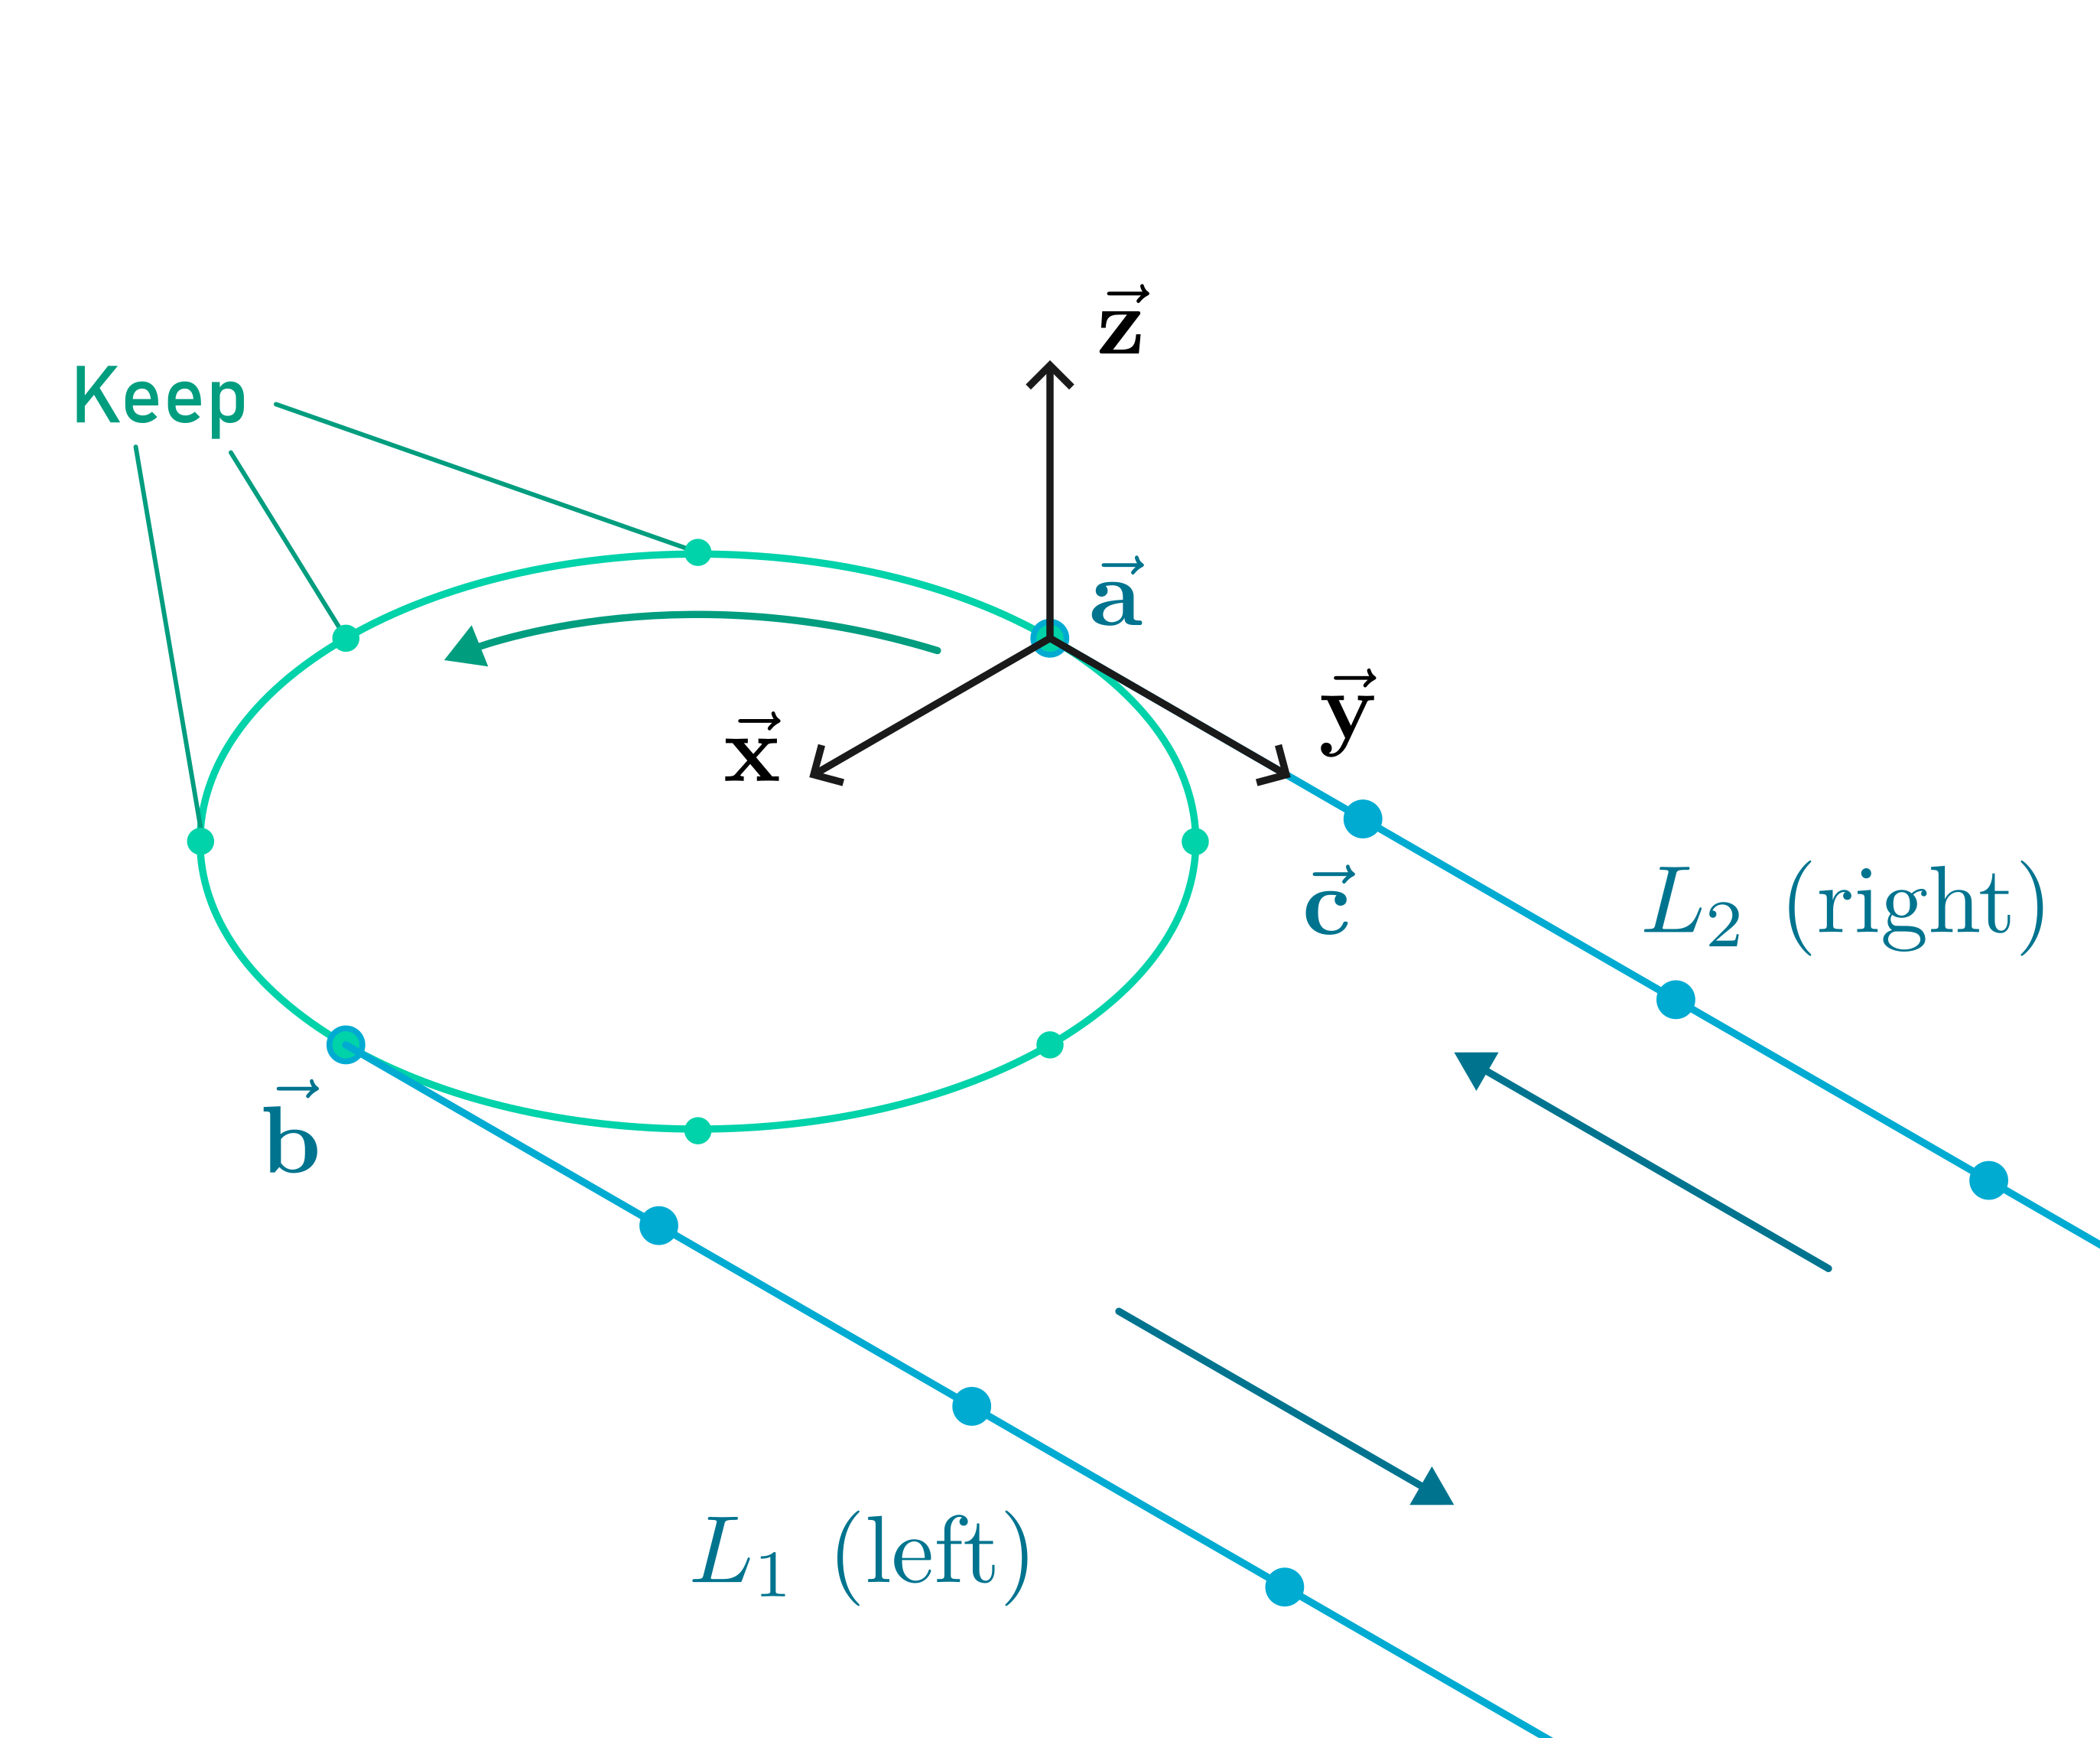
\includegraphics[width=0.7\textwidth]{Swath-Edge.png} 
    \caption{Swath Edge Illustration}
    \label{fig:swath-edge}
\end{figure}

%\newcommand{\a}{$\sesv{a}$} 

\newcommand{\Fs}{$\vec{\mathcal{F}}_s$} 
%\newcommand{\Fe}{$\vec{\mathcal{F}}_E$}

This is the procedure for finding the `outside' points on one end of a swath as
illustrated in Figure~\ref{fig:swath-edge}. First, we take the two last points
of the boundary lines, $\sev{a}$ and $\sev{b}$, defined in \gls{ecef}
coordinates, \Fe. If we look down the length of a swath towards the end we are
calculating ellipse points for, $\sev{a}$ is on the right and $\sev{b}$ is on
the left.  Let us also take a third point, $\sev{c}$, which is the second last
point on the right boundary line.  From these points, we can to define a
coordinate reference frame, \Fs $= [\sev{x}, \sev{y}, \sev{z}]$, with respect
to \Fe, where:

\begin{equation}
    \sev{x} = \frac{\sev{b}-\sev{a}}{\norm{\sev{b} - \sev{a}}}
    , \quad
    \sev{y} = \frac{\sev{c}-\sev{a}}{\norm{\sev{c} - \sev{a}}}
    , \quad
    \sev{z} = \sev{x} \times \sev{y}
\end{equation}

In this reference frame, all of the ellipse points that are outside the swath
will have negative y-components. To determine this, we can project each point
in the ellipse onto the x-y plane of \Fs~and then take the dot product of the
projected point with $\sev{y}$. To order the edge points such that they
correctly form the boundary, we can take the dot product of the projected point
and $\sev{x}$ and then store them in ascending order. This procedure yields
the algorithm in Algorithm~\ref{alg:swath-edge}.

%% NOTE: this is not how it's defined in the code. Here it's been reversed for clarity

\begin{algorithm}
    \caption{Swath Edge Algorithm} 
    \label{alg:swath-edge}
    \begin{algorithmic}[1] 
	\Function{SwathEdge}{$L_1, L_2, E$}
	\Let{$\sev{a}$}{$L_2[-1]$}	\Comment{Last Point}
	\Let{$\sev{b}$}{$L_1[0]$}	\Comment{First Point}
	\Let{$\sev{c}$}{$L_2[-2]$}	\Comment{Second Last Point}
	\Let{$\sev{x}$}{$\sev{b}-\sev{a}/\norm{\sev{b}-\sev{a}}$}
	\Let{$\sev{y}$}{$\sev{c}-\sev{a}/\norm{\sev{c}-\sev{a}}$}
	\Let{$\sev{z}$}{$\sev{x} \times \sev{y}$}

	\ForEach{Ellipse Point $\sev{e}$ in $E$}
	    \Let{$\sesv{p}{e}$}{$\sev{e} - (\sev{e}\cdot\sev{z})\sev{z}$} 
	    \Comment{Projection onto x-z plane}

	    \If {$(\sesv{p}{e} \cdot \sev{y}) < 0 $}
		\Let{$O$}{\Call{InsertSorted}{$\sev{e}$, $(\sesv{p}{e}\cdot\sev{x})$, $O$}}
		\Comment{Sort in Descending order}
	    \EndIf
	\EndFor
	\State \Return $O$
	\EndFunction
    \end{algorithmic} 
\end{algorithm}

When providing points to this algorithm, it is assumed that the points in $L_1$
and $L_2$ are ordered Counter Clockwise. Also, sorting algorithms are not the
focus here so the implementation of \textsc{InsertSorted} has been omitted for
clarity.  This was the procedure for finding the swath edge for the start of
the swath.  To find the edge for the end, we can use the same algorithm but
switch $L_1$ and $L_2$, and pass the Ellipse at the end of the swath. In so
doing, we have flipped $L_1$ to be the right side of the swath instead of the
left and vice-versa for $L_2$. 

%%%%%%%%%%%%%%%%%%%%%%%%%%%%%%%%%%%%%%%%%%%%%%%%%%%%%%%%%%%%%%%%%%%%%%%%%%%%%% 

%\section{Counter-Clockwise Reordering Algorithm} \label{alg:ccw}

%%%%%%%%%%%%%%%%%%%%%%%%%%%%%%%%%%%%%%%%%%%%%%%%%%%%%%%%%%%%%%%%%%%%%%%%%%%%%% 

%\section{Convex Polygon Conversion} \label{alg:force-complex}

           

	
% ******************Appendix*******************
%\appendix
\begin{appendices}
    %\glsresetall{} 
\appendix

\chapter{Algorithms} \label{chap:Algorithms}

%\lettrine[lines=2, findent=0pt, nindent=5pt]{T}{} 

Through the development of the \gls{pops}, a number of algorithms have been
developed to perform various functions. These algorithms are not necessarily
ground breaking but their implementations are novel and worth discussing in
some form. To avoid detracting from the main body of the thesis they are
discussed here, in the appendix.


\section{Multiple Access Intersection Algorithm} \label{alg:mul-access-inter}

For some search scenarios, \gls{pops} may need to determine for what times do all
satellites have access to a target such as an \gls{aoi} or a ground station.
That is, if there are multiple satellites and each satellite has a list of
access times to a target, \gls{pops} must generate a new list of access times where
each access corresponds to a period where all satellites have access. An
example scenario is illustrated in Figure~\ref{fig:access_intersect}.


\begin{figure}[h]
    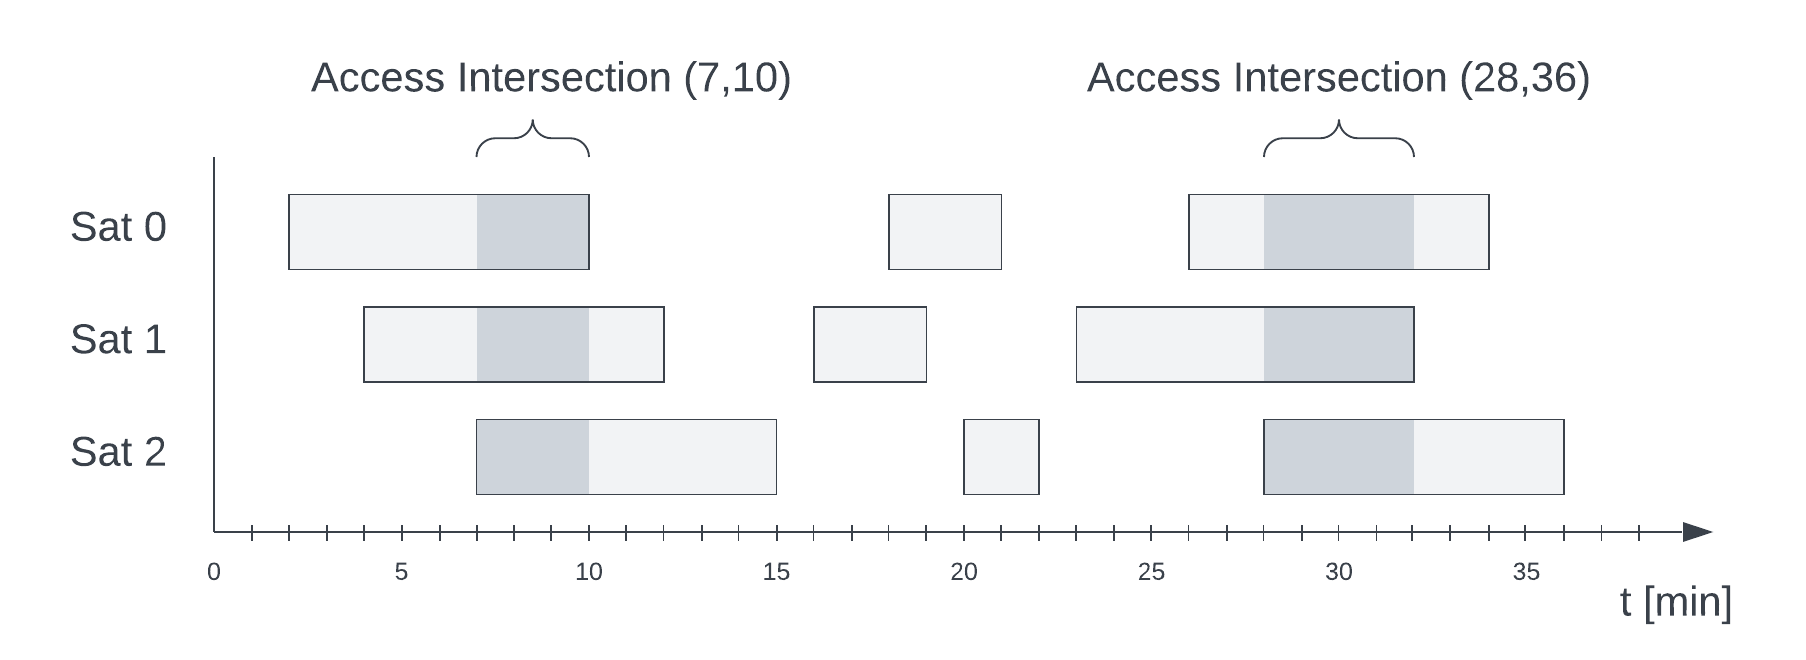
\includegraphics[width=\textwidth]{Access Intersection Example.png} 
    \caption{Illustration of a Potential Access Intersection Scenario}
\label{fig:access_intersect}
\end{figure}

In this scenario, there are three satellites: Sat 0, Sat 1, and Sat 2. Each has
multiple access periods represented with gray boxes. Though time is continuous,
it has been discretized into integer timesteps for simplicity. Minutes have
been selected as the units for time but this is arbitrary. From these lists of
access periods, this algorithm must determine all of the points in time where
all satellites have an access period. For the example scenario, the outputted
results should be $[7,10]$ and $[28,36]$. Note that between $t = 16$ and $t=22$
there are access overlaps but since there are only overlaps between two
satellites, they should not be returned as intersection periods.

For each satellite, access times are stored as a list of timestamps. Every even
and odd indexed timestamp specifies when the satellite `enters' and `leaves' an
access respectively. Access lists $\ses{a}{n}$ can be described generally for
satellite $n$ as,

\begin{equation}\label{eq:access-list} 
    \ses{a}{n} = \left[ a_{n,0}, b_{n,0}, a_{n,1}, b_{n,1}, \ldots a_{n,m}, b_{n,m} \right]
\end{equation}


where $a$ is the access enter timestamp, $b$ is the access leave timestamp, and
$m$ is the number of accesses. We also make the assumption that no accesses
overlap for a given satellite and target; that is,

\begin{equation}\label{eq:access-list-constraint}
    a_{n,0} < b_{n,0} < a_{n,1} < b_{n,1} < \ldots < a_{n,m} < b_{n,m}
\end{equation}

One simple brute force solution to this problem would be to iterate over every
time step, $t$, and check if there exists an access region, $[a_n,b_n]$, for all
satellites, $n$, such that $t$ is between $a$ and $b$.

This solution is, of course, very wasteful as it scales with the number of
timesteps that are being considered, $\Theta(t)$. The number of timesteps may
be on the order of 1,000s to 10,000s of timesteps. A simplification can be made
since we do not need to actually consider every timestep. Rather, we can
instead iterate over the access boundaries since they describe continuous
periods of time. By focusing on just the access boundaries, we may develop an
algorithm which scales with the number of accesses, $\Theta(m)$, which is much
smaller than the total number of timesteps.

For all satellite access lists we are considering, let us combine them into two
$1\times nm$ arrays. The first `timestamp' array, $\se{b}$, contains a sorted
list of all of the boundary timestamps in ascending order. The second `index'
array, $\se{s}$, contains a list of satellite indices in the same order as the
timestamp array. For example,

\begin{equation*}
    \begin{aligned} 
	\ses{a}{0} &= \left[ 2, 10, 18, 21  \right] \\
	\ses{a}{1} &= \left[ 4, 12, 16, 19  \right] \\
	\ses{a}{2} &= \left[ 7, 15, 20, 22  \right] \\
    \end{aligned}
    \quad \Rightarrow \quad
    \left \{ 
	\begin{aligned}
	    \se{b} &= [ 2 , 4 , 7 , 10 , 12 , 15 , 16 , 18 , 19 , 20 , 21 , 22  ] \\
	    \se{s} &= [ 0 , 1 , 2 , 0 , 1 , 2 , 1 , 0 , 1 , 2 , 0 , 2  ]
	\end{aligned}
    \right.
\end{equation*}

Note these are some of the values from Figure \ref{fig:access_intersect}.
Again, in the actual implementation of the algorithm we use actual timestamps
but here we are using integers for demonstration purposes. The timestamp array
stores the timestamp of the access boundary for later reference and also gives
us the order of the satellite index array. Remember that access boundaries are
listed in order of [enter, leave, enter, leave, ...]. Looking at the first four
elements in the index array, $[0, 1, 2, 0]$, satellite 0 enters an access at
the first element and leaves the access at the fourth element. So for the
second and third element, satellite 0 still has access because it has not left
yet. In essence, the index array encodes in what order satellites enter and
leave accesses. 

Now let us expand on the index array so we can perform logical operations to
find intersections. For this the algorithm makes use of logic arrays.  These
are arrays which contain only Boolean values, True or False. With these arrays,
we can also perform logical operations on any axis. For example, if we have a 2
dimensional logic array, we can produce a 1 dimensional array, that is the
result of AND'ing all of the elements in each column. These allow us to perform
logical operations very quickly for many elements. From the index array let us
construct an $n\times nm$ boolean array, $\se{A}$, that describes our scenario.
The rows of matrix, $\se{A}$, correspond to the indices of each satellite.  For
example row 0 is satellite 0, row $m$ is satellite $m$, etc. The columns
correspond to elements in the index array, $\se{s}$.

Let us initialize $\se{A}$ to be all False values represented as 0s. Then,
starting at the first column of $\se{A}$, let us NOT the element in the
$\se{s}(0)$ row.  Then, for then next column, let us copy all of the values
from the previous column and again NOT the $\se{s}(1)$ element. This is then
repeated for all columns in $\se{A}$. There is one small catch, if we are
transitioning a 1 to a 0 or a True to a False, this should be done on the
following iteration. This essentially means that we are treating accesses in in
access boundaries as inclusive. Even if the satellite is leaving an access, we
say that it has access until the timestep immediately after the boundary. As an
example, let us construct $\se{A}$ from $\se{s}$ for all of Figure
\ref{fig:access_intersect},

\begin{equation*} 
    \se{s} = 
    \left[
    \begin{array}{cccccccccccccccccc}
	0 & 1 & 2 & 0 & 1 & 2 & 1 & 0 & 1 & 2 & 0 & 2 & 1 & 0 & 2 & 1 & 0 & 2 \\
    \end{array}
    \right]
\end{equation*}
yields,
\begin{equation*} 
    \se{A} = 
    \left[
	\begin{array}{cc;{2pt/2pt}cc;{2pt/2pt}cccccccccc;{2pt/2pt}cc;{2pt/2pt}cc}
	1 & 1 & 1 & 1 & 0 & 0 & 0 & 1 & 1 & 1 & 1 & 0 & 0 & 1 & 1 & 1 & 1 & 0 \\
	0 & 1 & 1 & 1 & 1 & 0 & 1 & 1 & 1 & 0 & 0 & 0 & 1 & 1 & 1 & 1 & 0 & 0 \\
	0 & 0 & 1 & 1 & 1 & 1 & 0 & 0 & 0 & 1 & 1 & 1 & 0 & 0 & 1 & 1 & 1 & 1 \\
    \end{array}
    \right]
\end{equation*}
Then, if we AND all of the rows in $\se{A}$ we get,
\begin{equation*} 
    \se{A}' = 
    \left[
    \begin{array}{cccccccccccccccccc}
	0 & 0 & 1 & 1 & 0 & 0 & 0 & 0 & 0 & 0 & 0 & 0 & 0 & 0 & 1 & 1 & 0 & 0 \\
    \end{array}
    \right]
\end{equation*}
It is clear to see that this matrix gives us the indices where there is an
intersection between all satellites. If we take all values of $\se{b}$ where
$\se{A}'$ is True, we are left with,
\begin{equation*} 
    \se{b}' = 
    \left[
    \begin{array}{cccccccccccccccccc}
	7 & 10 & 28 & 32
    \end{array}
    \right]
\end{equation*}
which is our expected result. This was just a walkthrough but the explicit
algorithm definition is defined in Algorithm~\ref{alg:access-intersection}.

\begin{algorithm}[h] 
    \caption{Access Intersection} 
    \label{alg:access-intersection}
    \begin{algorithmic}[1]
	%\Require{\se{z}is a $1\times N$ array } 
	\Function{AccessIntersection}{$\ses{a}{0}$,$\ses{a}{1}$, ... , $\ses{a}{n}$} 

	    \Let{$\se{s}$, $\se{b}$}{\Call{Combine}{$\ses{a}{0}$,$\ses{a}{1}$, ... , $\ses{a}{n}$}}  

	    \Let{$l$}{\Call{Length}{$\se{s}$}}

	    \Let{$\se{A}$}{\Call{Zeros}{$n$,$l$}}

	    %\Let{$\se{A}[\se{s}[0],0]$}{1}  \Comment{Set up the first column}
	    \Let{$\se{t}$}{$\se{A}[:,0]$} \Comment{Temporary array to store column of $\se{A}$}

	    \Let{$i$}{0} \Comment{Boundary iterator}

	    \While{$i \neq m$}
		\Let{$s$}{$\se{s}[i]$} \Comment{Satellite index}
		
		\If{!$\se{t}$($s$)}
		\Let{$\se{t}$($s$)}{!$\se{t}$($s$)}
		    \Comment{Flip element then copy values over}
		    \Let{$\se{A}[:,s]$}{\Call{OR}{$\se{A}[:,s]$, $\se{t}$}} 
		\Else
		    \Let{$\se{A}[:,s]$}{\Call{OR}{$\se{A}[:,s]$, $\se{t}$}} 
		    \Comment{Copy values over then flip element}
		    \Let{$\se{t}$($s$)}{!$\se{t}$($s$)}
		\EndIf


		\Let{$i$}{$i+1$}
	    \EndWhile 

	    \Let{$\se{a}'$}{\Call{ColumnsAND}{$\se{A}$}}

	    \Let{$\se{b}'$}{$\se{b}[\se{a}']$} \Comment{Select indices based on logical value}

	\State \Return $\se{b}'$
	\EndFunction
    \end{algorithmic}


\end{algorithm}

For this algorithm, the implementation of \textsc{Combine} function was omitted
for clarity since it is an implementation detail. Also, note that this
algorithm is not limited to only access intersections but it may also calculate
unions by replacing \textsc{ColumnsAND} with \textsc{ColumnsOR} in line 18.

%%%%%%%%%%%%%%%%%%%%%%%%%%%%%%%%%%%%%%%%%%%%%%%%%%%%%%%%%%%%%%%%%%%%%%%%%%%%%% 

%\section{Equator Crossing Algorithm} \label{sec:equator-crossing}
%
%For a given ephemeris, it is useful to determine each `pass' of that orbit.
%That is, for each ephemeris point, an index should be assigned to it which
%indicates how many times the spacecraft has orbited the Earth. In this way, if
%we have some time range and we wish to see the next `pass,' we would simply
%take that time range's pass index and add 1.
%
%There are many ways a pass may be defined. For example, we could specify a
%latitude and longitude range and whenever the spacecraft is in this range, that
%could be considered a singular pass.  Generally, though, ephemeris data is not
%given in latitude or longitude, rather it is given in a Cartesian position in
%some \gls{eci} or \gls{ecef} coordinate reference frame. So, for each position
%in the ephemeris, the position vector will need to be converted to latitude and
%longitude. 
%
%This is a completely acceptable approach but we may also simplify the problem.
%Instead of taking a latitude and longitude range, we could instead increment
%the pass index when the spacecraft crosses the equator and goes from the
%southern to the northern hemisphere. This would be when the spacecraft's
%position goes from a negative to a positive latitude. This definition of a pass
%has a few advantages. That being, we only need to do one check to determine a
%pass boundary. It also has the benefit of indexing the entire ephemeris. Still
%for this method, we need to convert from Cartesian position to at least
%latitude.
%
%Let us make one further simplification by assuming that the x-y plane of the
%ephemeris's coordinate system is very near to the Earth's equatorial plane.
%This is not true for all coordinate systems but it is true for the \gls{ecef}
%ephemerides used by \gls{pops}. By making this assumption, we no longer need to
%calculate the latitude of the spacecraft; rather, we can instead only look at
%the spacecraft's position along the z-axis. This is useful because the
%spacecraft's z-position will oscillate between some positive and negative
%extrema, which are determined by the orbit's inclination and eccentricity. 
%
%There is a complicating factor that should be accounted for. In time, the
%spacecraft's position is periodic, but when considering only the spacecraft's
%z-position in an ephemeris, there is no guarantee that there is a constant
%timestep between position values. Additional data-points may be injected for
%periods where greater accuracy is desired and vice-versa. 
%
%We may now articulate the problem to be addressed: Given, an array of
%$z$-positions, $\se{z}$, generate a new array, $\se{p}$, that each element of
%$\se{p}$ is the index of an element in $\se{z}$ after a crossover occurs (i.e.\
%the positive value in the negative-to-positive crossing). To determine if
%elements, $n$ and $m$, of an array, $\se{z}$, form a crossover, they must
%satisfy three simple conditions:
%
%\begin{enumerate}
%    \item $\se{z}[n] < 0$
%    \item $\se{z}[m] > 0$ 
%    \item $m = n+1$
%\end{enumerate}
%
%
%A brute-force approach to finding $\se{p}$ would be to loop through all of the
%elements in $\se{z}$ and test them against the above conditions. This method,
%though, is inelegant and may be computationally intensive.  
%
%Alternatively, we can instead try and make use of 
%
%Another approach to
%this problem is outlined in Algorithm~\ref{alg:crossover}.  In essence, it
%attempts to reduce the number of comparisons made to search for crossovers. 
%
%\begin{algorithm}[h] 
%    \caption{Negative-Positive Crossing Search Algorithm} 
%    \label{alg:crossover}
%    \begin{algorithmic}[1] 
%	\Require{\se{z}is a $1\times N$ array } 
%
%	\Function{FindAllCrossovers}{$s, f, \se{z}$}
%	    \Let{$p$}{\Call{FindNextCrossover}{$0, s, f, \se{z}$}} \Comment{Start at beginning of array}
%	    \Let{$\se{p}$}{$\{ p \}$}
%
%	    \While{$p \neq -1$}
%		\Let{$p$}{\Call{FindNextCrossover}{$p, s, f, \se{z}$}}
%		\Comment{Start at beginning of array} \State
%		$\se{p}$.append($p$) \EndWhile 
%		\State \Return \se{p}
%	\EndFunction
%
%	\State
%
%	\Function{FindNextCrossover}{$i, s, f, \se{z}$} 
%	\Let{$j$}{$i+s$}
%	\If{$j > length(\se{z})$} 
%	    \State $s = \mathrm{s \times f}$  
%	\ElsIf{$j = length(\se{z})$}
%	    \State \Return $-1$	  \Comment{Search has completed}
%	\ElsIf{ $(\se{z}[i] < 0) \lor (\se{z}[j] > 0)$ }
%	    \If{$s=1$}
%	    \State \Return $i$ \Comment{Crossover index found}
%	    \Else
%		\State $s = ceil(s \times f)$
%	    \EndIf
%	\Else
%	    \State $i=j$
%	\EndIf
%	\State \Return \Call{FindNextCrossover}{$i, s, f, \se{z}$}
%	\EndFunction 
%    \end{algorithmic} 
%\end{algorithm}


%%%%%%%%%%%%%%%%%%%%%%%%%%%%%%%%%%%%%%%%%%%%%%%%%%%%%%%%%%%%%%%%%%%%%%%%%%%%%% 

\section{Single Access Intersection Algorithm} \label{alg:contains}

The Single Access Intersection Algorithm is similar to the Multiple Access
Intersection algorithm but it serves a different purpose. Given a time range,
this algorithm is concerned with finding all of the access times in a list that
intersect that time range. Here, the input time range will not be used as
bounds, but only search criteria to select access times. 

\begin{figure}[h]
    \centering
    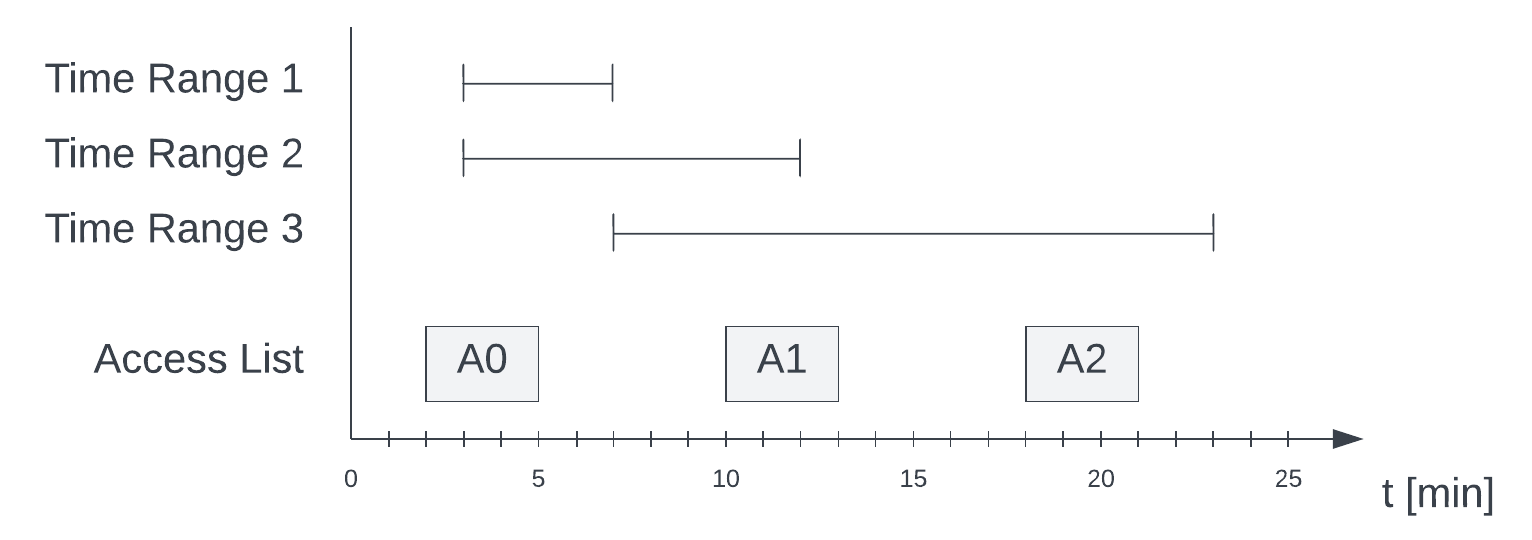
\includegraphics[width=\textwidth]{Single Access.png} 
    \caption{Illustration of a Potential Single Intersection Scenarios}
    \label{fig:single-access-intersect}
\end{figure}

To get a better idea of the problem, let us look at some more concrete example
scenarios. Figure~\ref{fig:single-access-intersect} illustrates an access list
as well as three possible input time ranges, time range 1-3. For time range 1,
the output should be merely A0. For time range 2, the output will be A0 and A1.
Lastly, time range 3 will have outputs A1 and A2. Notice here that the limits
of the time range may lie within or without an access. As long as the access
intersects the time range at all, it should be included.

The two inputs to this algorithm are a time region with boundaries $\alpha$ and
$\beta$ where $\alpha < \beta$. The access list, $\se{a}$, is the same as
described in Equation~\ref{eq:access-list} where the subscript, $n$ has been
omitted since only one access list is to be considered. Additionally, the
assumption in Equation~\ref{eq:access-list-constraint} still holds here. It
should be emphasized that given an access list, every even entry is an access
enter timestamp and every odd entry is an access leave timestamp.

The main intuition for this problem is that we must first constrain the list of
access boundaries to the those boundaries that lie within the time range.
Then, we must assemble the access times from their boundaries and output them
in a list.  

First we find two values, $i$ and $j$.  These are the indices of the next
smallest value for $\alpha$ and $\beta$ in the access list.  For example, in
time range 2, from Figure~\ref{fig:single-access-intersect}, $i$ and $j$ will
be the indices of $a_0$ and $a_1$ respectively. These two values will be used
to create an iteration range that will be used to return the list of accesses. 

One problem is that, as they are, $i$ may not point to an access enter and $j$
may not point to an access leave which is required by access lists. So, if $i$
points to an access enter, nothing should be done but if it points to an access
leave, it should be incremented to point to the next access enter. Similarly,
if $j$ points to an access leave nothing should be done, but if it points to an
access enter it should be incremented as well.  To address this, we may take
advantage of the access list's even and oddness as mentioned earlier.  With
modular arithmetic, we can select the correct indices,

\begin{align*}
    i' &= i + \mathrm{mod}(i,2) \\
    j' &= j + \mathrm{mod}(j+1,2)
\end{align*}
where $i'$ and $j'$ are the shifted indices and `mod()' is the modulus
function.  The first argument is the dividend and the second is the divisor.
Once we have these values, the output will be the access times that lie within
the range $[i', j']$. All together, the algorithm can be seen in
Algorithm~\ref{alg:single-access-intersection}.


\begin{algorithm}[h] 
    \caption{Single Access Intersection}
    \label{alg:single-access-intersection} 
    \begin{algorithmic}[1]
	%\Require{\se{z}is a $1\times N$ array } 
	\Function{SingleAccessIntersection}{$\alpha$, $\beta$, $\se{a}$} 

	\Let{$i$}{$\se{a}[-1]$}
	\Let{$j$}{$\se{a}[-1]$} \Comment{Initialize}

	\ForEach{$t$ in $\se{a}$} \Comment{Find next smallest }
	    \If{ $t < \alpha$ }
	    \Let{$i$}{$t$}  
	    \EndIf
	    \If{ $t < \beta$ }
		\Let{$j$}{$t$}
	    \EndIf
	\EndFor

	\Let{$i'$}{$i + \mathrm{mod}(i,2)$} \Comment{Increment indices}
	\Let{$j'$}{$i + \mathrm{mod}(j+1,2)$} 

	\If{$i > j$}
	    \State \Return $[]$ \Comment{No Access Found}
	\Else
	    \State \Return $\se{a}[i',j']$ \Comment{Return list of access times}
	\EndIf
	\EndFunction
    \end{algorithmic}
\end{algorithm}

This algorithm is very simple and straightforward but it still serves a useful
function. Determining if ground station accesses lie between two accesses may
be calculated hundreds of times in a single search, so it is important that
this calculation is quick and efficient.


%%%%%%%%%%%%%%%%%%%%%%%%%%%%%%%%%%%%%%%%%%%%%%%%%%%%%%%%%%%%%%%%%%%%%%%%%%%%%% 

\section{Swath Boundary Ellipse Algorithm} \label{alg:ellipse}

To review, Swaths are the area covered by a satellite's \gls{fov} footprint or
\gls{for} access region over time. They are calculated from a satellite
ephemeris, where for each telemetry point in the ephemeris, two swath boundary
points are generated. By combining these points together over an entire
ephemeris, we are given two polylines which form the boundaries of the swath,
$L_1$ and $L_2$. If we look in the same direction and the velocity vector of
the satellite at a single time instant, $L_1$ is to the left and $L_2$ is to
the right. Though this is not always the case, the \gls{fov} or \gls{for} of
satellites in \gls{pops} are assumed to be conical. As such, for each ephemeris
point the swath is calculated from, an elliptical footprint/access region is
approximated through a list of some number of points. For clarity, these points
grouped together are referred to as an `Ellipse', $E$, just so that we do not
need to distinguish between footprints and access regions.  

Suppose we wish to more accurately display a swath by including the ellipse
points at the boundaries. Our main problem is that we must determine what
points in the first, $E_{start}$, and last, $E_{end}$ ellipse lie `outside' of the
swath.  If they are inside the swath, they provide no new information and do
not lie on the boundary.  We must also omit points on the ellipses that can be
found on the boundary lines since they are already accounted for. Also, for
robustness, let us assume that the list of points in each Ellipse are not
necessarily in order. This may be the case but this saves us from having to
rely on convention which may be broken in the future.

\begin{figure}[h]
    \centering
    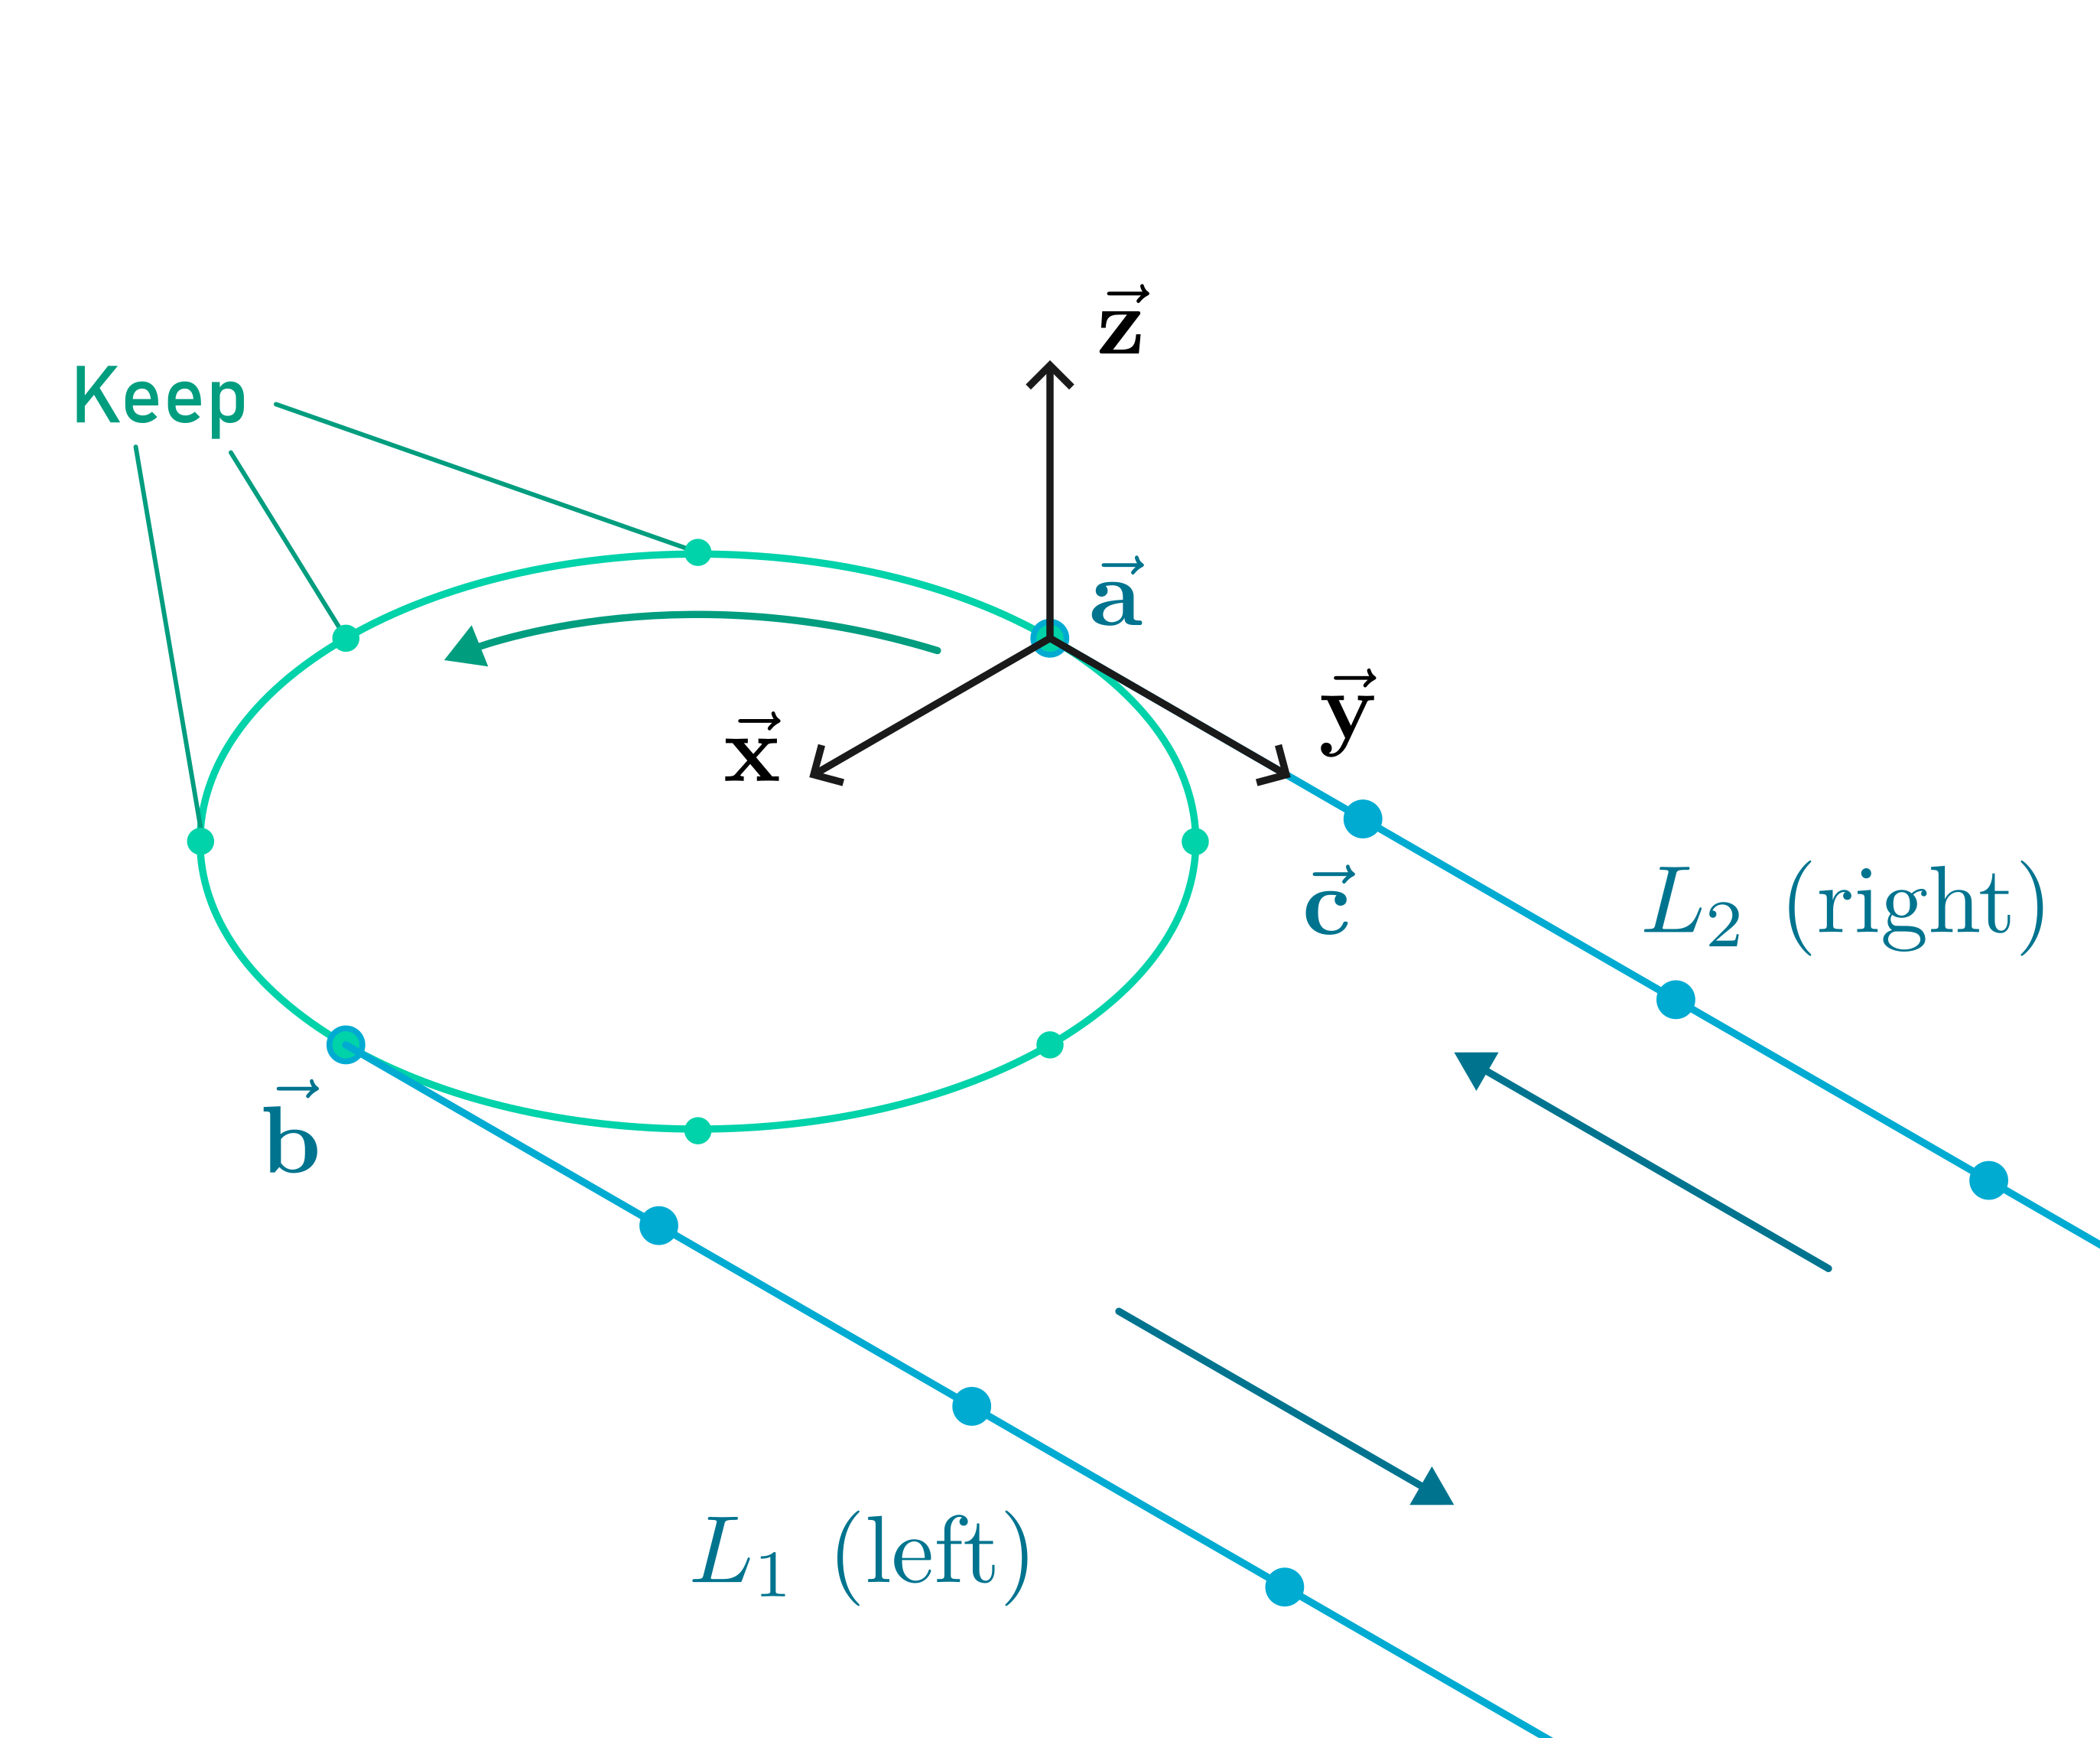
\includegraphics[width=0.7\textwidth]{Swath-Edge.png} 
    \caption{Swath Edge Illustration}
    \label{fig:swath-edge}
\end{figure}

%\newcommand{\a}{$\sesv{a}$} 

\newcommand{\Fs}{$\vec{\mathcal{F}}_s$} 
%\newcommand{\Fe}{$\vec{\mathcal{F}}_E$}

This is the procedure for finding the `outside' points on one end of a swath as
illustrated in Figure~\ref{fig:swath-edge}. First, we take the two last points
of the boundary lines, $\sev{a}$ and $\sev{b}$, defined in \gls{ecef}
coordinates, \Fe. If we look down the length of a swath towards the end we are
calculating ellipse points for, $\sev{a}$ is on the right and $\sev{b}$ is on
the left.  Let us also take a third point, $\sev{c}$, which is the second last
point on the right boundary line.  From these points, we can to define a
coordinate reference frame, \Fs $= [\sev{x}, \sev{y}, \sev{z}]$, with respect
to \Fe, where:

\begin{equation}
    \sev{x} = \frac{\sev{b}-\sev{a}}{\norm{\sev{b} - \sev{a}}}
    , \quad
    \sev{y} = \frac{\sev{c}-\sev{a}}{\norm{\sev{c} - \sev{a}}}
    , \quad
    \sev{z} = \sev{x} \times \sev{y}
\end{equation}

In this reference frame, all of the ellipse points that are outside the swath
will have negative y-components. To determine this, we can project each point
in the ellipse onto the x-y plane of \Fs~and then take the dot product of the
projected point with $\sev{y}$. To order the edge points such that they
correctly form the boundary, we can take the dot product of the projected point
and $\sev{x}$ and then store them in ascending order. This procedure yields
the algorithm in Algorithm~\ref{alg:swath-edge}.

%% NOTE: this is not how it's defined in the code. Here it's been reversed for clarity

\begin{algorithm}
    \caption{Swath Edge Algorithm} 
    \label{alg:swath-edge}
    \begin{algorithmic}[1] 
	\Function{SwathEdge}{$L_1, L_2, E$}
	\Let{$\sev{a}$}{$L_2[-1]$}	\Comment{Last Point}
	\Let{$\sev{b}$}{$L_1[0]$}	\Comment{First Point}
	\Let{$\sev{c}$}{$L_2[-2]$}	\Comment{Second Last Point}
	\Let{$\sev{x}$}{$\sev{b}-\sev{a}/\norm{\sev{b}-\sev{a}}$}
	\Let{$\sev{y}$}{$\sev{c}-\sev{a}/\norm{\sev{c}-\sev{a}}$}
	\Let{$\sev{z}$}{$\sev{x} \times \sev{y}$}

	\ForEach{Ellipse Point $\sev{e}$ in $E$}
	    \Let{$\sesv{p}{e}$}{$\sev{e} - (\sev{e}\cdot\sev{z})\sev{z}$} 
	    \Comment{Projection onto x-z plane}

	    \If {$(\sesv{p}{e} \cdot \sev{y}) < 0 $}
		\Let{$O$}{\Call{InsertSorted}{$\sev{e}$, $(\sesv{p}{e}\cdot\sev{x})$, $O$}}
		\Comment{Sort in Descending order}
	    \EndIf
	\EndFor
	\State \Return $O$
	\EndFunction
    \end{algorithmic} 
\end{algorithm}

When providing points to this algorithm, it is assumed that the points in $L_1$
and $L_2$ are ordered Counter Clockwise. Also, sorting algorithms are not the
focus here so the implementation of \textsc{InsertSorted} has been omitted for
clarity.  This was the procedure for finding the swath edge for the start of
the swath.  To find the edge for the end, we can use the same algorithm but
switch $L_1$ and $L_2$, and pass the Ellipse at the end of the swath. In so
doing, we have flipped $L_1$ to be the right side of the swath instead of the
left and vice-versa for $L_2$. 

%%%%%%%%%%%%%%%%%%%%%%%%%%%%%%%%%%%%%%%%%%%%%%%%%%%%%%%%%%%%%%%%%%%%%%%%%%%%%% 

%\section{Counter-Clockwise Reordering Algorithm} \label{alg:ccw}

%%%%%%%%%%%%%%%%%%%%%%%%%%%%%%%%%%%%%%%%%%%%%%%%%%%%%%%%%%%%%%%%%%%%%%%%%%%%%% 

%\section{Convex Polygon Conversion} \label{alg:force-complex}


\end{appendices}
    	
% ******************Back Matter*******************
\backmatter{}
%%\nocite{zee}
%\nocite{Sinclair}
%\nocite{ThermalControl}
%\nocite{HeatAndMass}
%\nocite{instar1}
%\nocite{instar3}
%\nocite{instar4}
%\nocite{instar5}
%\nocite{clean}
%\nocite{esd}
%\nocite{stm}
%\nocite{staking}
\printbibliography[heading=bibintoc, title= {References}]
\end{document}
